\documentclass[letter,10pt]{article}
\usepackage[utf8]{inputenc}
\usepackage[english]{babel}
\usepackage{float}
\usepackage{graphicx}
\usepackage{caption}
\usepackage{subcaption}
\usepackage{amsmath}
\usepackage{multirow}
\usepackage{color}
\usepackage{tabularx}
\usepackage{geometry}
\usepackage{capt-of}
% \renewcommand\floatpagefraction{0.9}
\title{Supporting information for:\\ Deep convolutional networks for quality assessment of protein folds}
\author{}

\renewcommand*{\thefigure}{S\arabic{figure}}
\renewcommand*{\thetable}{S\arabic{table}}

\begin{document}

\maketitle


\begin{figure}[H]
    \centering
    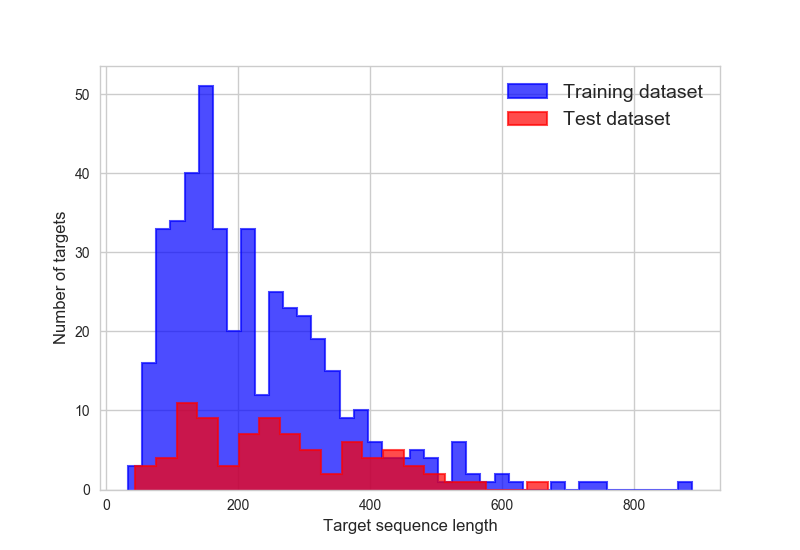
\includegraphics[width=\linewidth]{Fig/datasetLengthDistributions.png}
    \caption{Distributions of sequence lengths for targets in training set (blue) and test set (red).}
    \label{Fig:dataLengthDist}
\end{figure}

\begin{table}[H]
\begin{center}
%
    \caption{Closest homolog sequences from the training set.
      sequence pair is reported if at least one training sequence
      aligns to a test sequence with a blastp E-value less than
      $10^{-4}$. Only the top alignment is reported for each test
      sequence.}
%
\begin{tabular}{ c | c | l }
    
    Test set ID & Closest training set ID & E-value \\
    \hline
    T0768 & T0690 & $2.70\times 10^{-13}$ \\
    T0770 & T0645 & $1.79\times 10^{-13}$ \\
    T0772 & T0518 & $1.89\times 10^{-7}$ \\
    T0776 & T0707 & $3.98\times 10^{-5}$ \\
    T0783 & T0699 & $1.19\times 10^{-22}$ \\
    T0798 & T0308 & $9.57\times 10^{-6}$ \\
    T0813 & T0398 & $2.45\times 10^{-5}$ \\
    T0819 & T0636 & $8.66\times 10^{-15}$ \\
    T0854 & T0324 & $2.13\times 10^{-13}$ \\
\end{tabular}
\label{Tbl:datasetsSimilarity}
\end{center}
\end{table}


\begin{table}[H]
\begin{center}
\caption{Targets from test and training sets that belong to the same
  Pfam family \cite{finn2016pfam}, based on a HMMER search
  \cite{finn2015hmmer} with an E-value cutoff of 1.0. With that
  cutoff, 403 of the 564 training targets and 65 of the 83 test
  targets could be assigned families. There are 25 families containing
  at least one test sequence and one training sequence, involving a
  total of 16 test targets and 42 training targets. Each of the 25
  families belongs to a distinct Pfam clan.}
%
\begin{tabular}{ l | l | l }

    Common & Test set target & Training set targets \\
    family & & \\
    \hline
    PF00795 & T0794 & T0542 \\ \hline
    PF13472 & T0776 & T0448, T0297, T0286, T0750 \\ \hline
    PF03807 & T0813 & T0398, T0393, T0702 \\ \hline
    PF00266 & T0801 & T0339, T0697 \\ \hline
    PF01128 & T0783 & T0699, T0420 \\ \hline
    PF07949 & T0780 & T0572 \\ \hline
    PF13577 & T0815 & T0752, T0736 \\ \hline
    PF12804 & T0783 & T0593, T0699, T0420 \\ \hline
    PF13242 & T0854 & T0371, T0341, T0303, T0324, T0330, T0329, T0418 \\ \hline
    PF13306 & T0768 & T0690, T0671, T0713, T0653 \\ \hline
    PF12741 & T0770 & T0664, T0645, T0532 \\ \hline
    PF00025 & T0798 & T0308 \\ \hline
    PF12872 & T0792 & T0549 \\ \hline
    PF03446 & T0813, T0851 & T0398, T0393, T0702 \\ \hline
    PF00155 & T0801, T0819 & T0591, T0636, T0436, T0697 \\ \hline
    PF13419 & T0854 & T0371, T0341, T0303, T0379, T0324, T0330, T0329, T0418, T0635 \\ \hline
    PF12680 & T0815 & T0451, T0475 \\ \hline
    PF06439 & T0772 & T0518 \\ \hline
    PF12771 & T0770 & T0664, T0645, T0532 \\ \hline
    PF08477 & T0798 & T0308 \\ \hline
    PF00657 & T0776 & T0297, T0286, T0679 \\ \hline
    PF00071 & T0798 & T0308 \\ \hline
    PF00702 & T0854 & T0303, T0324, T0330, T0329, T0418, T0635 \\ \hline
    PF01926 & T0798 & T0308 \\ \hline
    PF12697 & T0764 & T0672 \\ \hline
\end{tabular}
\label{Tbl:SharedPfam}
\end{center}
\end{table}

% \begin{table}[H]
% \begin{center}
%
% \caption{Targets from CASP11 that do not have corresponding PDB
%   entries or ECOD classes.}
%
% \begin{tabular}{ l | l | l }

%     Target & Has PDB & Has ECOD class \\
%     \hline
%     T0773 &True &False\\
%     T0820 &False &False\\
%     T0823 &False &False\\
%     T0824 &False &False\\
%     T0827 &False &False\\
%     T0835 &False &False\\
%     T0836 &False &False\\
%     T0838 &False &False\\
% \end{tabular}
% \label{Tbl:CASP11PDB_ECOD}
% \end{center}
% \end{table}


\begin{figure}[H]
    \centering
    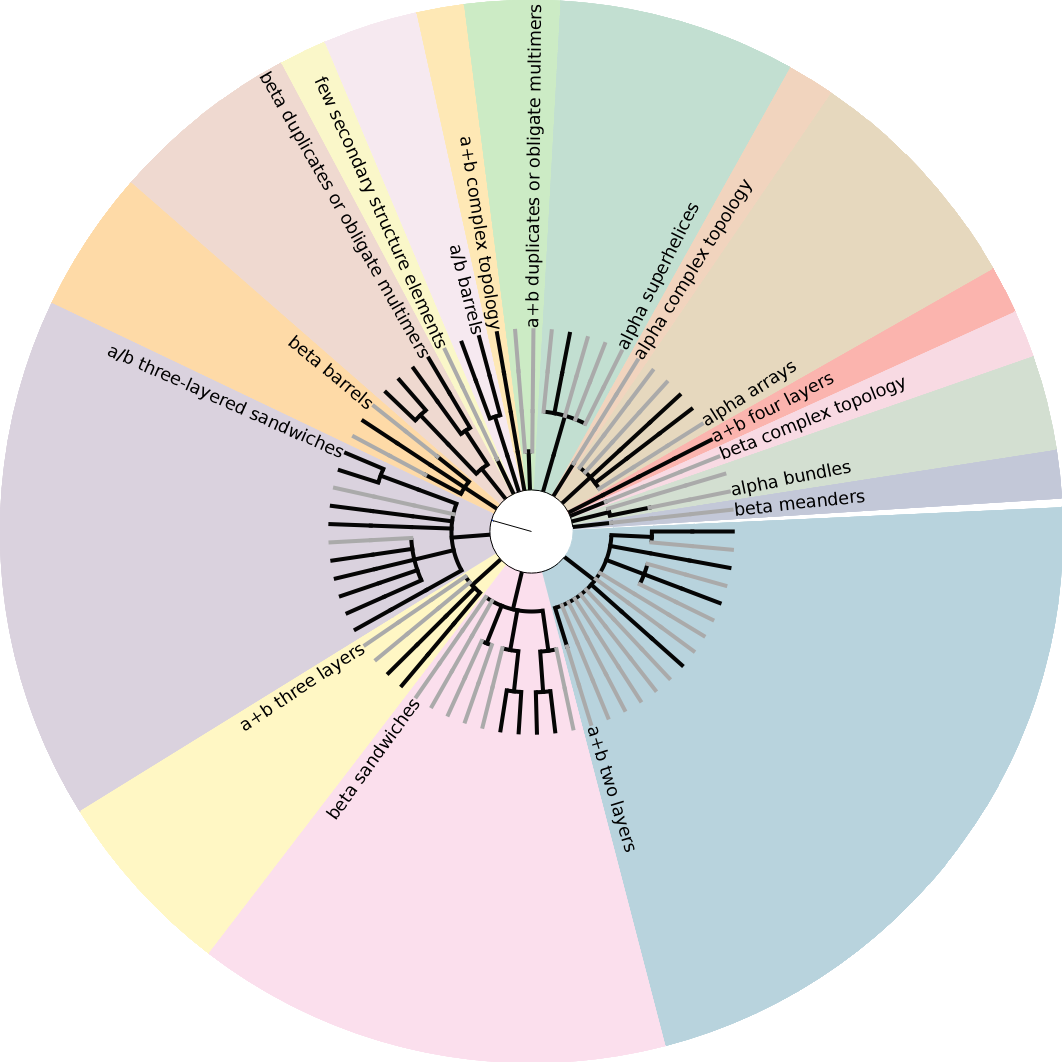
\includegraphics[width=\linewidth]{Fig/folds_graph.png}
%
    \caption{Classification of the test set structures into the top
      four ECOD structural levels (from the center out): architecture
      (A), possible homology (X), homology (H), and topology (T). The
      names of the architecture types are shown in the outer circle of
      the diagram. Branches drawn in black correspond to groups that
      have representatives in both training and test sets. Branches
      drawn in grey correspond to groups unique to the test set.
%
      Four architecture groups present overlap at all levels between
      the training and test sets: ``a/b barrels'', ``beta duplicates
      or obligate multimers'', ``a+b complex topology'', and ``a+b
      four layers''.
%
      We do not show the F-groups because they have litle overlap
      among the training and test sets.
%
      Targets T0773, T0797, and T0816 are excluded from the analysis
      because they have no ECOD classification, and targets T0820,
      T0823, T0824, T0827, T0835, and T0836 are excluded because they
      have no structure in the RCSB PDB.}
%
    \label{Fig:foldsGraph}
\end{figure}

\begin{table}[H]
\begin{center}
%
\caption{Details of the model architecture. Layer 10 is marked with an
  asterisk to indicate that its output was used in the Grad-CAM
  analysis reported in Section~4 of the main text.}
%
\makebox[0pt][c]{
\hskip-\footskip
\begin{tabularx}{0.8\paperwidth}{ l | l | c | c | c }

    Layer & Type & Input dimensions & Output dimensions & Parameters \\
    \hline
    1&3D Convolution & $11\times 120\times 120\times 120$ & $16\times 118\times 118\times 118$ & 
                    Filter size $3\times 3\times 3$, stride $1$\\
    2&ReLU & & & \\
    3&Max pooling & $16\times 118\times 118\times 118$ & $16\times 58\times 58\times 58$ & 
                    Filter size $3\times 3\times 3$, stride $2$ \\
    \hline 
    4&3D Convolution & $16\times 58\times 58\times 58$ & $32\times 56\times 56\times 56$ & 
                    Filter size $3\times 3\times 3$, stride $1$\\
    5&Batch normalization & & & \\
    6&ReLU & & & \\
    7&Max pooling & $32\times 56\times 56\times 56$ & $32\times 27\times 27\times 27$ & 
                    Filter size $3\times 3\times 3$, stride $2$ \\
    \hline
    8&3D Convolution & $32\times 27\times 27\times 27$ & $32\times 25\times 25\times 25$ & 
                    Filter size $3\times 3\times 3$, stride $1$\\
    9&Batch normalization & & & \\
    10*&ReLU & & & \\
    11&3D Convolution & $32\times 25\times 25\times 25$ & $64\times 23\times 23\times 23$ & 
                    Filter size $3\times 3\times 3$, stride $1$\\
    12&Batch normalization & & & \\
    13&ReLU & & & \\
    14&Max pooling & $64\times 23\times 23\times 23$ & $64\times 11\times 11\times 11$ & 
                    Filter size $3\times 3\times 3$, stride $2$ \\
    \hline
    15&3D Convolution & $64\times 11\times 11\times 11$ & $128\times 9\times 9\times 9$ & 
                    Filter size $3\times 3\times 3$, stride $1$\\
    16&Batch normalization & & & \\
    17&ReLU & & & \\
    18&3D Convolution & $128\times 9\times 9\times 9$ & $128\times 7\times 7\times 7$ & 
                    Filter size $3\times 3\times 3$, stride $1$\\
    19&Batch normalization & & & \\
    20&ReLU & & & \\
    21&3D Convolution & $128\times 7\times 7\times 7$ & $256\times 5\times 5\times 5$ & 
                    Filter size $3\times 3\times 3$, stride $1$\\
    22&Batch normalization & & & \\
    23&ReLU & & & \\
    24&3D Convolution & $256\times 5\times 5\times 5$ & $512\times 3\times 3\times 3$ & 
                    Filter size $3\times 3\times 3$, stride $1$\\
    25&Batch normalization & & & \\
    26&ReLU & & & \\
    27&Max pooling & $512\times 3\times 3\times 3$ & $512\times 1\times 1\times 1$ & 
                    Filter size $3\times 3\times 3$, stride $2$ \\
    \hline
    28&Reshape & $512\times 1\times 1\times 1$ & $512$ & \\
    \hline
    29&Linear & 512 & 256 & \\
    30&ReLU & & & \\
    31&Linear & 256 & 128 & \\
    32&ReLU & & & \\
    33&Linear & 128 & 1 & \\
    \hline

\end{tabularx}
\hskip\headheight
}
\label{Tbl:SuppModel}
\end{center}
\end{table}


\pagebreak
\section*{Training procedure}

\subsection*{Rotations}
The rotations were sampled in the following way:
\begin{enumerate}
\item Select three random uniform values $u_1, u_2, u_3 \in [0,1]$
\item Construct quaternion from them
\begin{eqnarray}
q_0 = \sqrt(1-u_1) \sin(2\pi  u_2) \\
q_1 = \sqrt(1-u_1) \cos(2\pi  u_2) \\
q_2 = \sqrt(u_1) \sin(2\pi  u_3) \\
q_3 = \sqrt(u_1) \cos(2\pi  u_3) 
\end{eqnarray}
\item Construct the corresponding rotation matrix
\end{enumerate}

\subsection*{Translations}
The translations were sampled according to the following algorithm:
\begin{enumerate}
\item Compute the bounding box of the atoms in the decoy
\item Translate the protein so that the center of the bounding box corresponds to the frame origin 
\item Rotate protein using random uniform rotation
\item Calculate the maximum shift along each axis:
$$
D_k = \tfrac{1}{2}\max\left[ 0, \tfrac{1}{2}S_k - \tfrac{1}{2}B_k \right], \quad k \in {x, y, z}
$$
where $S_k$ are input size along the axes x,y,z and $B_k$ are the bounding box sizes along the same axes.

\item Sample random uniform translation along each axis from the
  interval $[-\tfrac{1}{2}D_k, \tfrac{1}{2}D_k], k \in {x,y,z}$
\end{enumerate}

\subsection*{Training parameters}

The loss function is optimized using the Adam algorithm \cite{kingma2014adam},
with a learning rate of $0.0003$ and a learning rate decay of $0.01$.

% \pagebreak
\begin{figure}[H]

    \centering
    \makebox[0pt][c]{
    \hskip-\footskip
    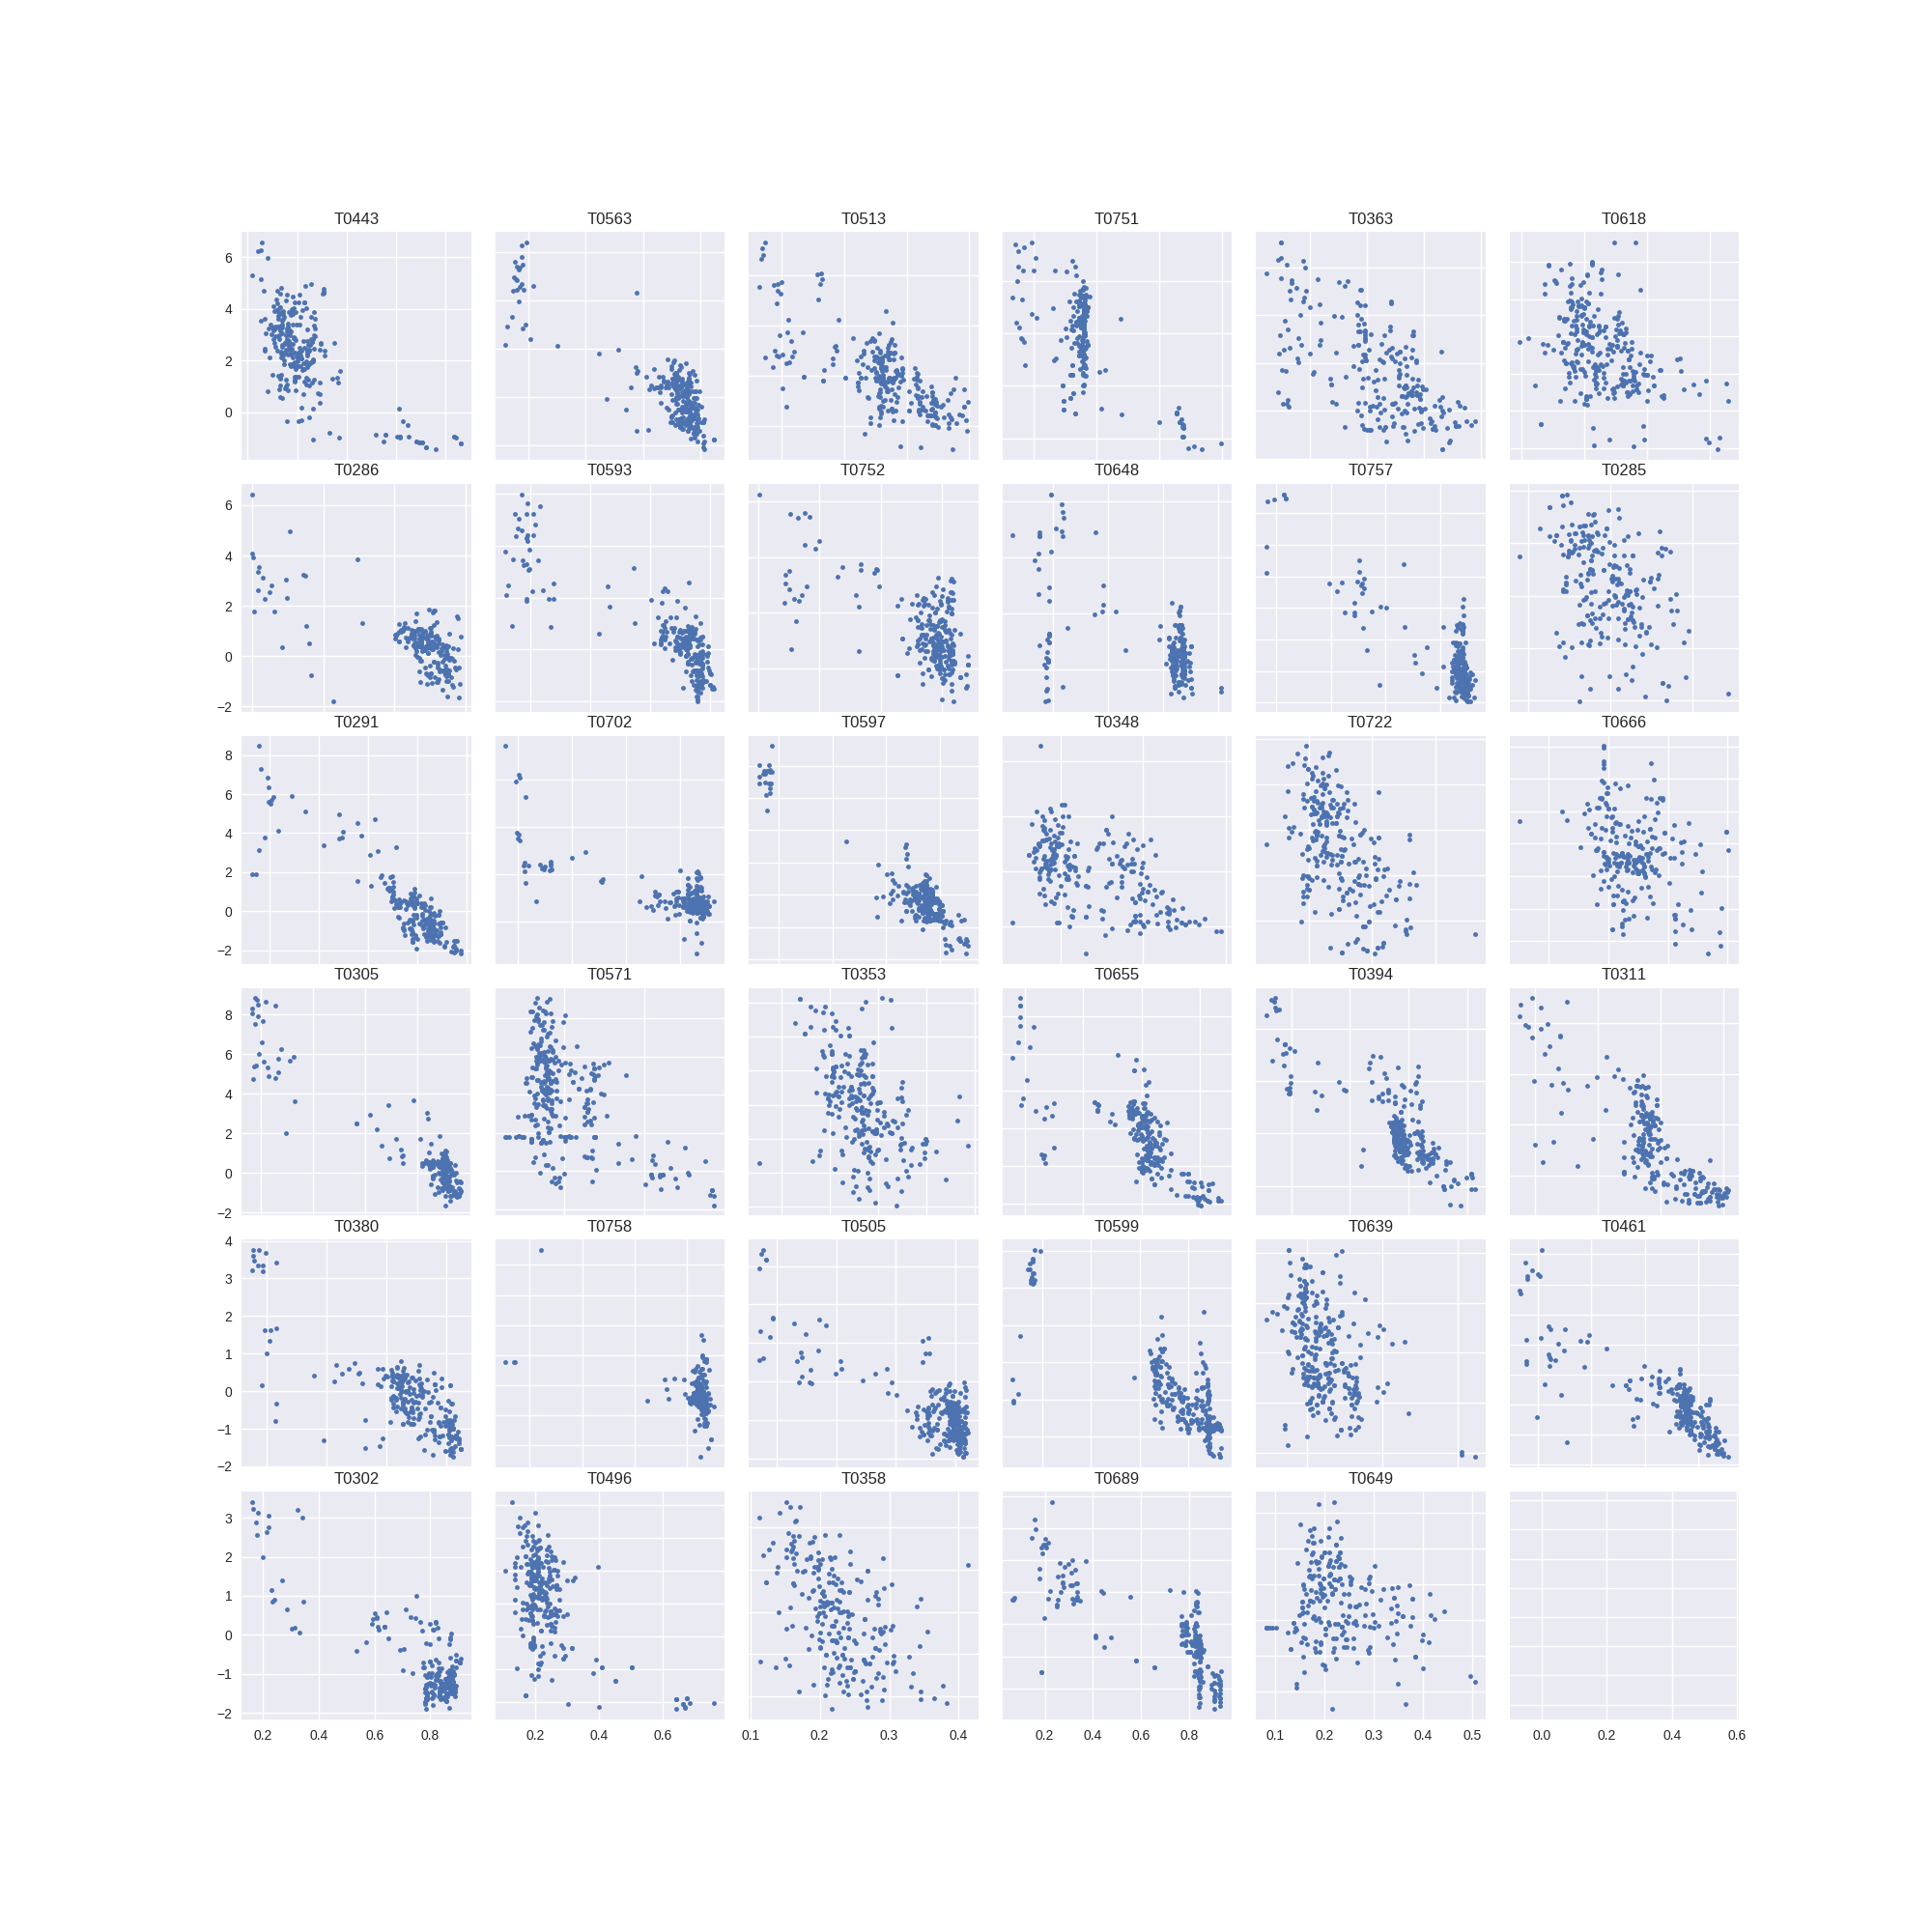
\includegraphics[width=0.8\paperwidth]{Fig/epoch40_funnels.png}
    \hskip\headheight
    }

    \caption{Scoring funnels on the validation set at epoch 40. The
      $x$-axis is the GDT\_TS score and the $y$-axis is the $f$
      score. The score was sampled once using random rotation and
      translation.}
%
    \label{Fig:ValidationEpoch40}
\end{figure}


%\section{Results}

\begin{figure}[H]
    \centering
    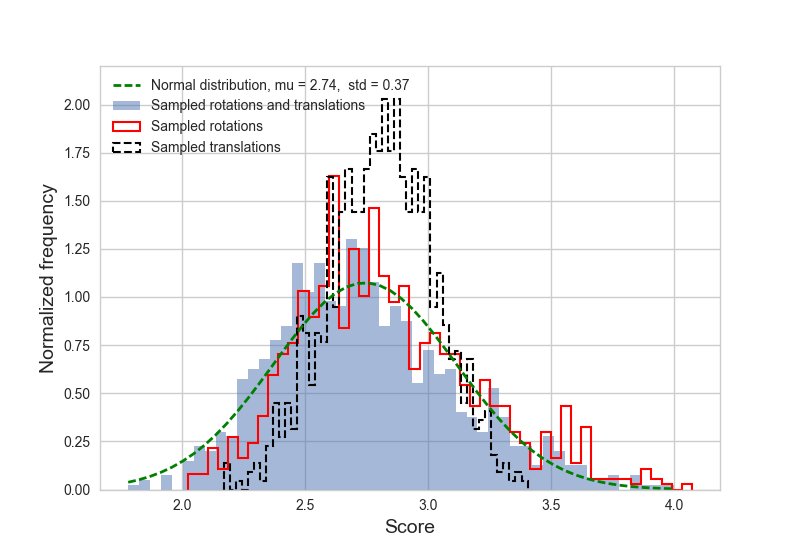
\includegraphics[width=\linewidth]{Fig/sampling_dist.eps}
%
    \caption{Distribution of the score of decoy FALCON\_EnvFold\_TS1
    for target T0832 under random translations and rotations. The
    distribution fits a normal distribution with an average $\mu =
    2.74$ and a standard deviation $\sigma = 0.37$ (shown in green
    dashed lines). The figure also shows the distributions of the
    score under rotations only (red lines) and under translations only
    (black dashed lines).}
%
    \label{Fig:ScoreDistribution}
\end{figure}


\begin{figure}[H]
    \centering
    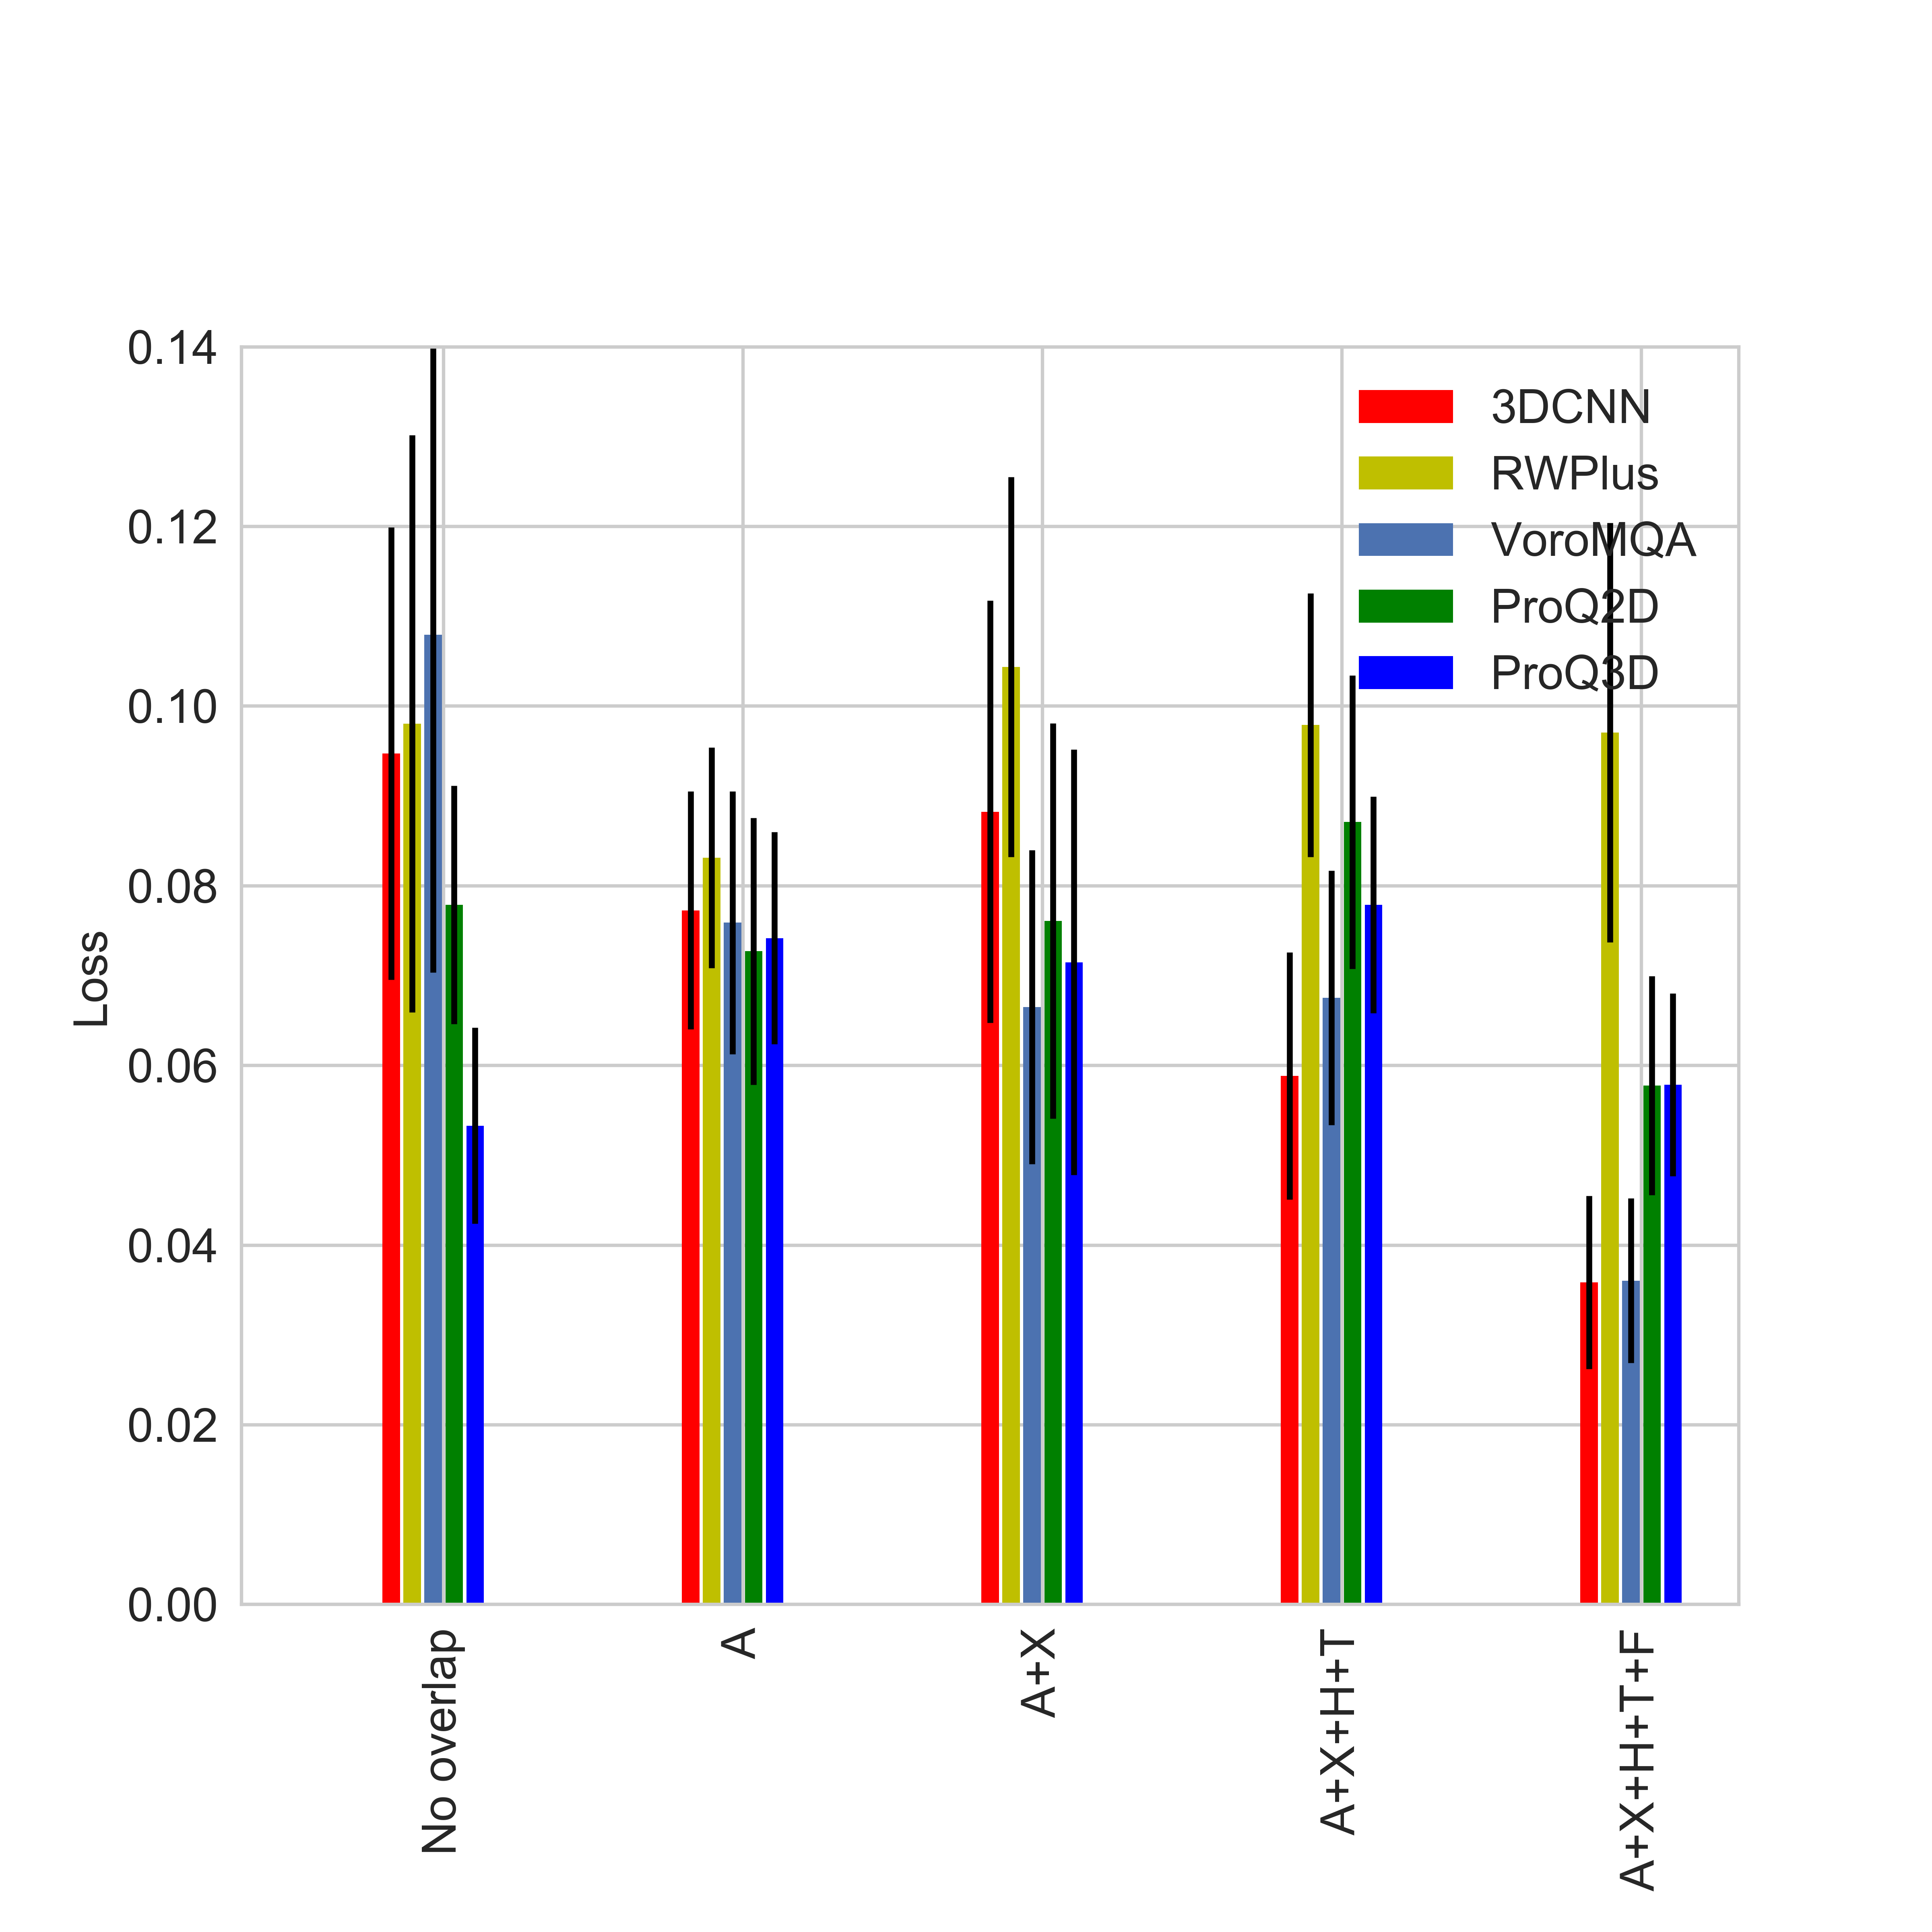
\includegraphics[width=\linewidth]{Fig/LossVsECOD.png}
%
    \caption{Per-target average loss of the MQA algorithms of Table~3
    on the CASP11 test set stage~2, divided into 5 subsets of
    increasing structural similarity with the training set. The
    subsets are chosen according to the presence in the training set
    of structures belonging to the same ECOD categories (see text for
    details). 
    ``No overlap'', the structures for which there is no structure in the training set with 
    the same ECOD (T0797 and T0773). 
    ``A'', the structures in the same A-group of at least one training
    structure but not in the same X-group (T0759, T0763, T0769, etc.); 
    ``A+X'', the structures in the same X-group of at least one training
    structure but not in the same H-group (T0760, T0761, T0765, etc.);
    ``A+X+H+T'', the structures in the same T-group of at least one
    training structure but not in the same F-group (T0762, T0766, T0767,
    etc.);
    ``A+X+H+T+F'', the structures in the same F-group of at least one
    training structure (T0764, T0768, T0770, etc.);
    Error bars show per-target standard error of mean of the loss.}
%
    \label{Fig:LossVsECOD}
\end{figure}

\begin{figure}[H]
    \centering
    \makebox[0pt][c]{
    \hskip-\footskip
    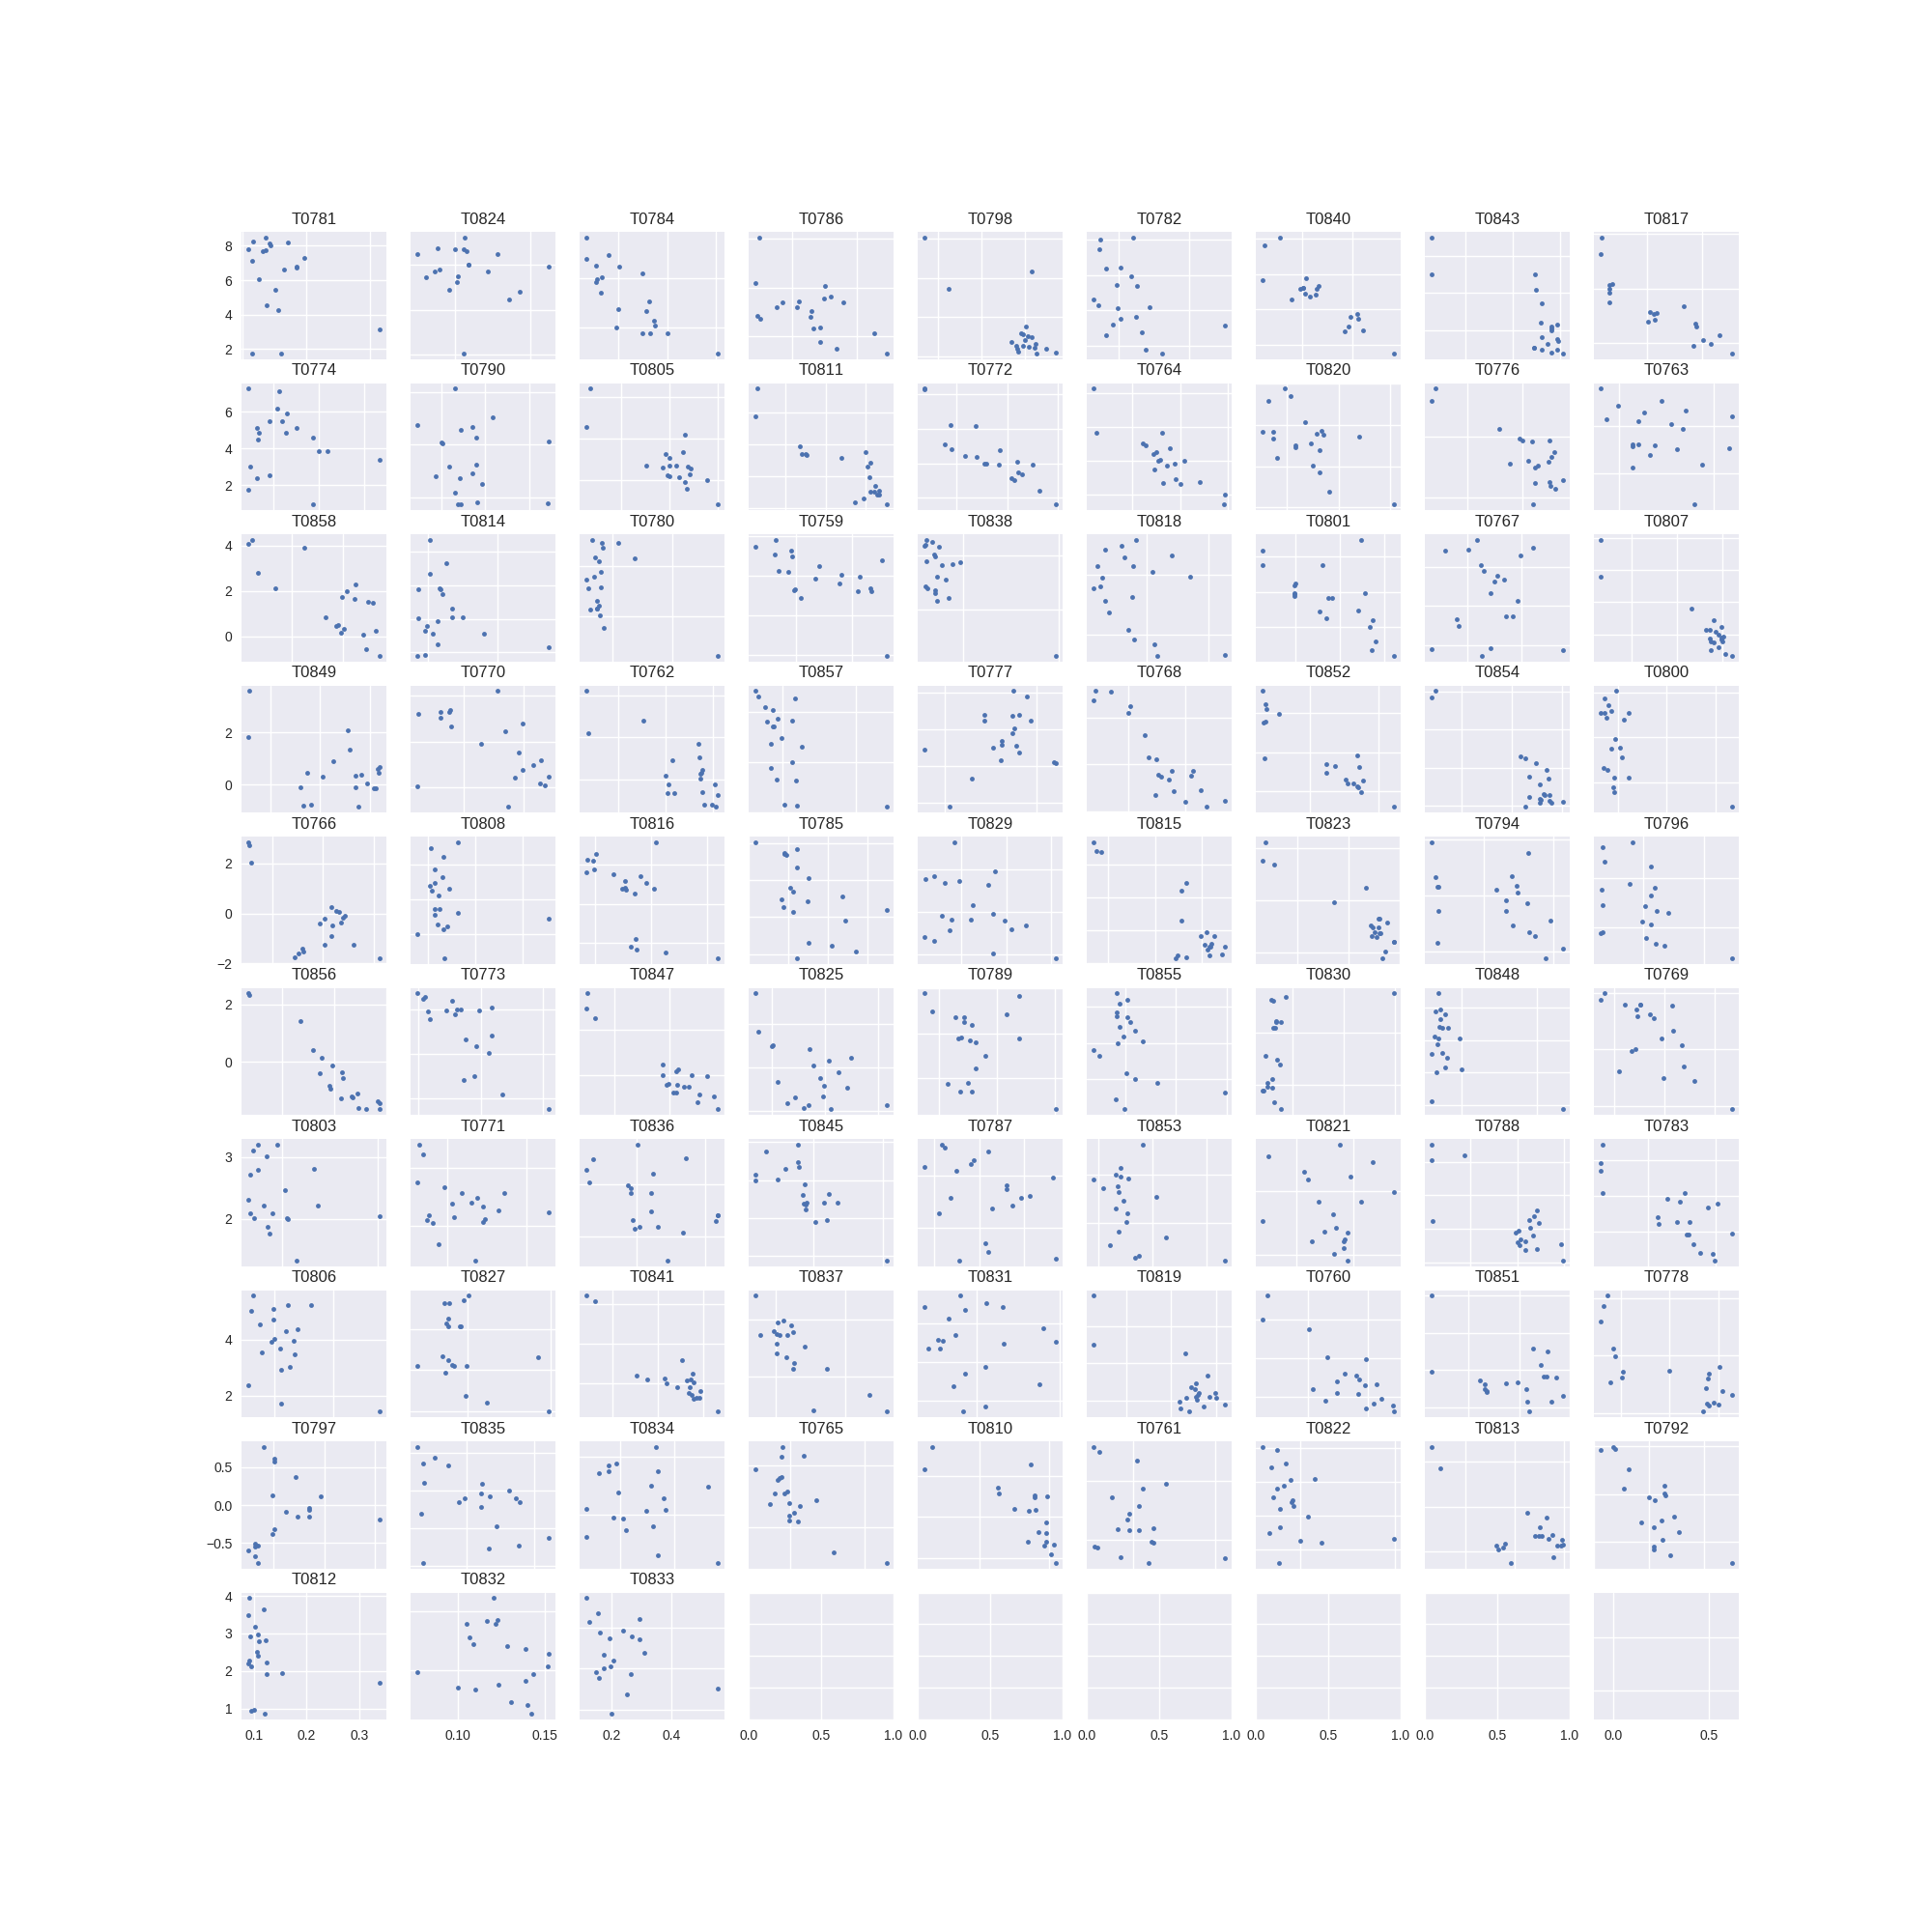
\includegraphics[width=0.9\paperwidth]{Fig/CASP11Stage1_SCWRL_sFinal_funnels.png}
    \hskip\headheight
    }
    \caption{Scoring funnels on Stage 1 CASP11}
    \label{Fig:Satage1CASP11Funnels}
\end{figure}

\begin{figure}[H]
    \centering
    \makebox[0pt][c]{
    \hskip-\footskip
    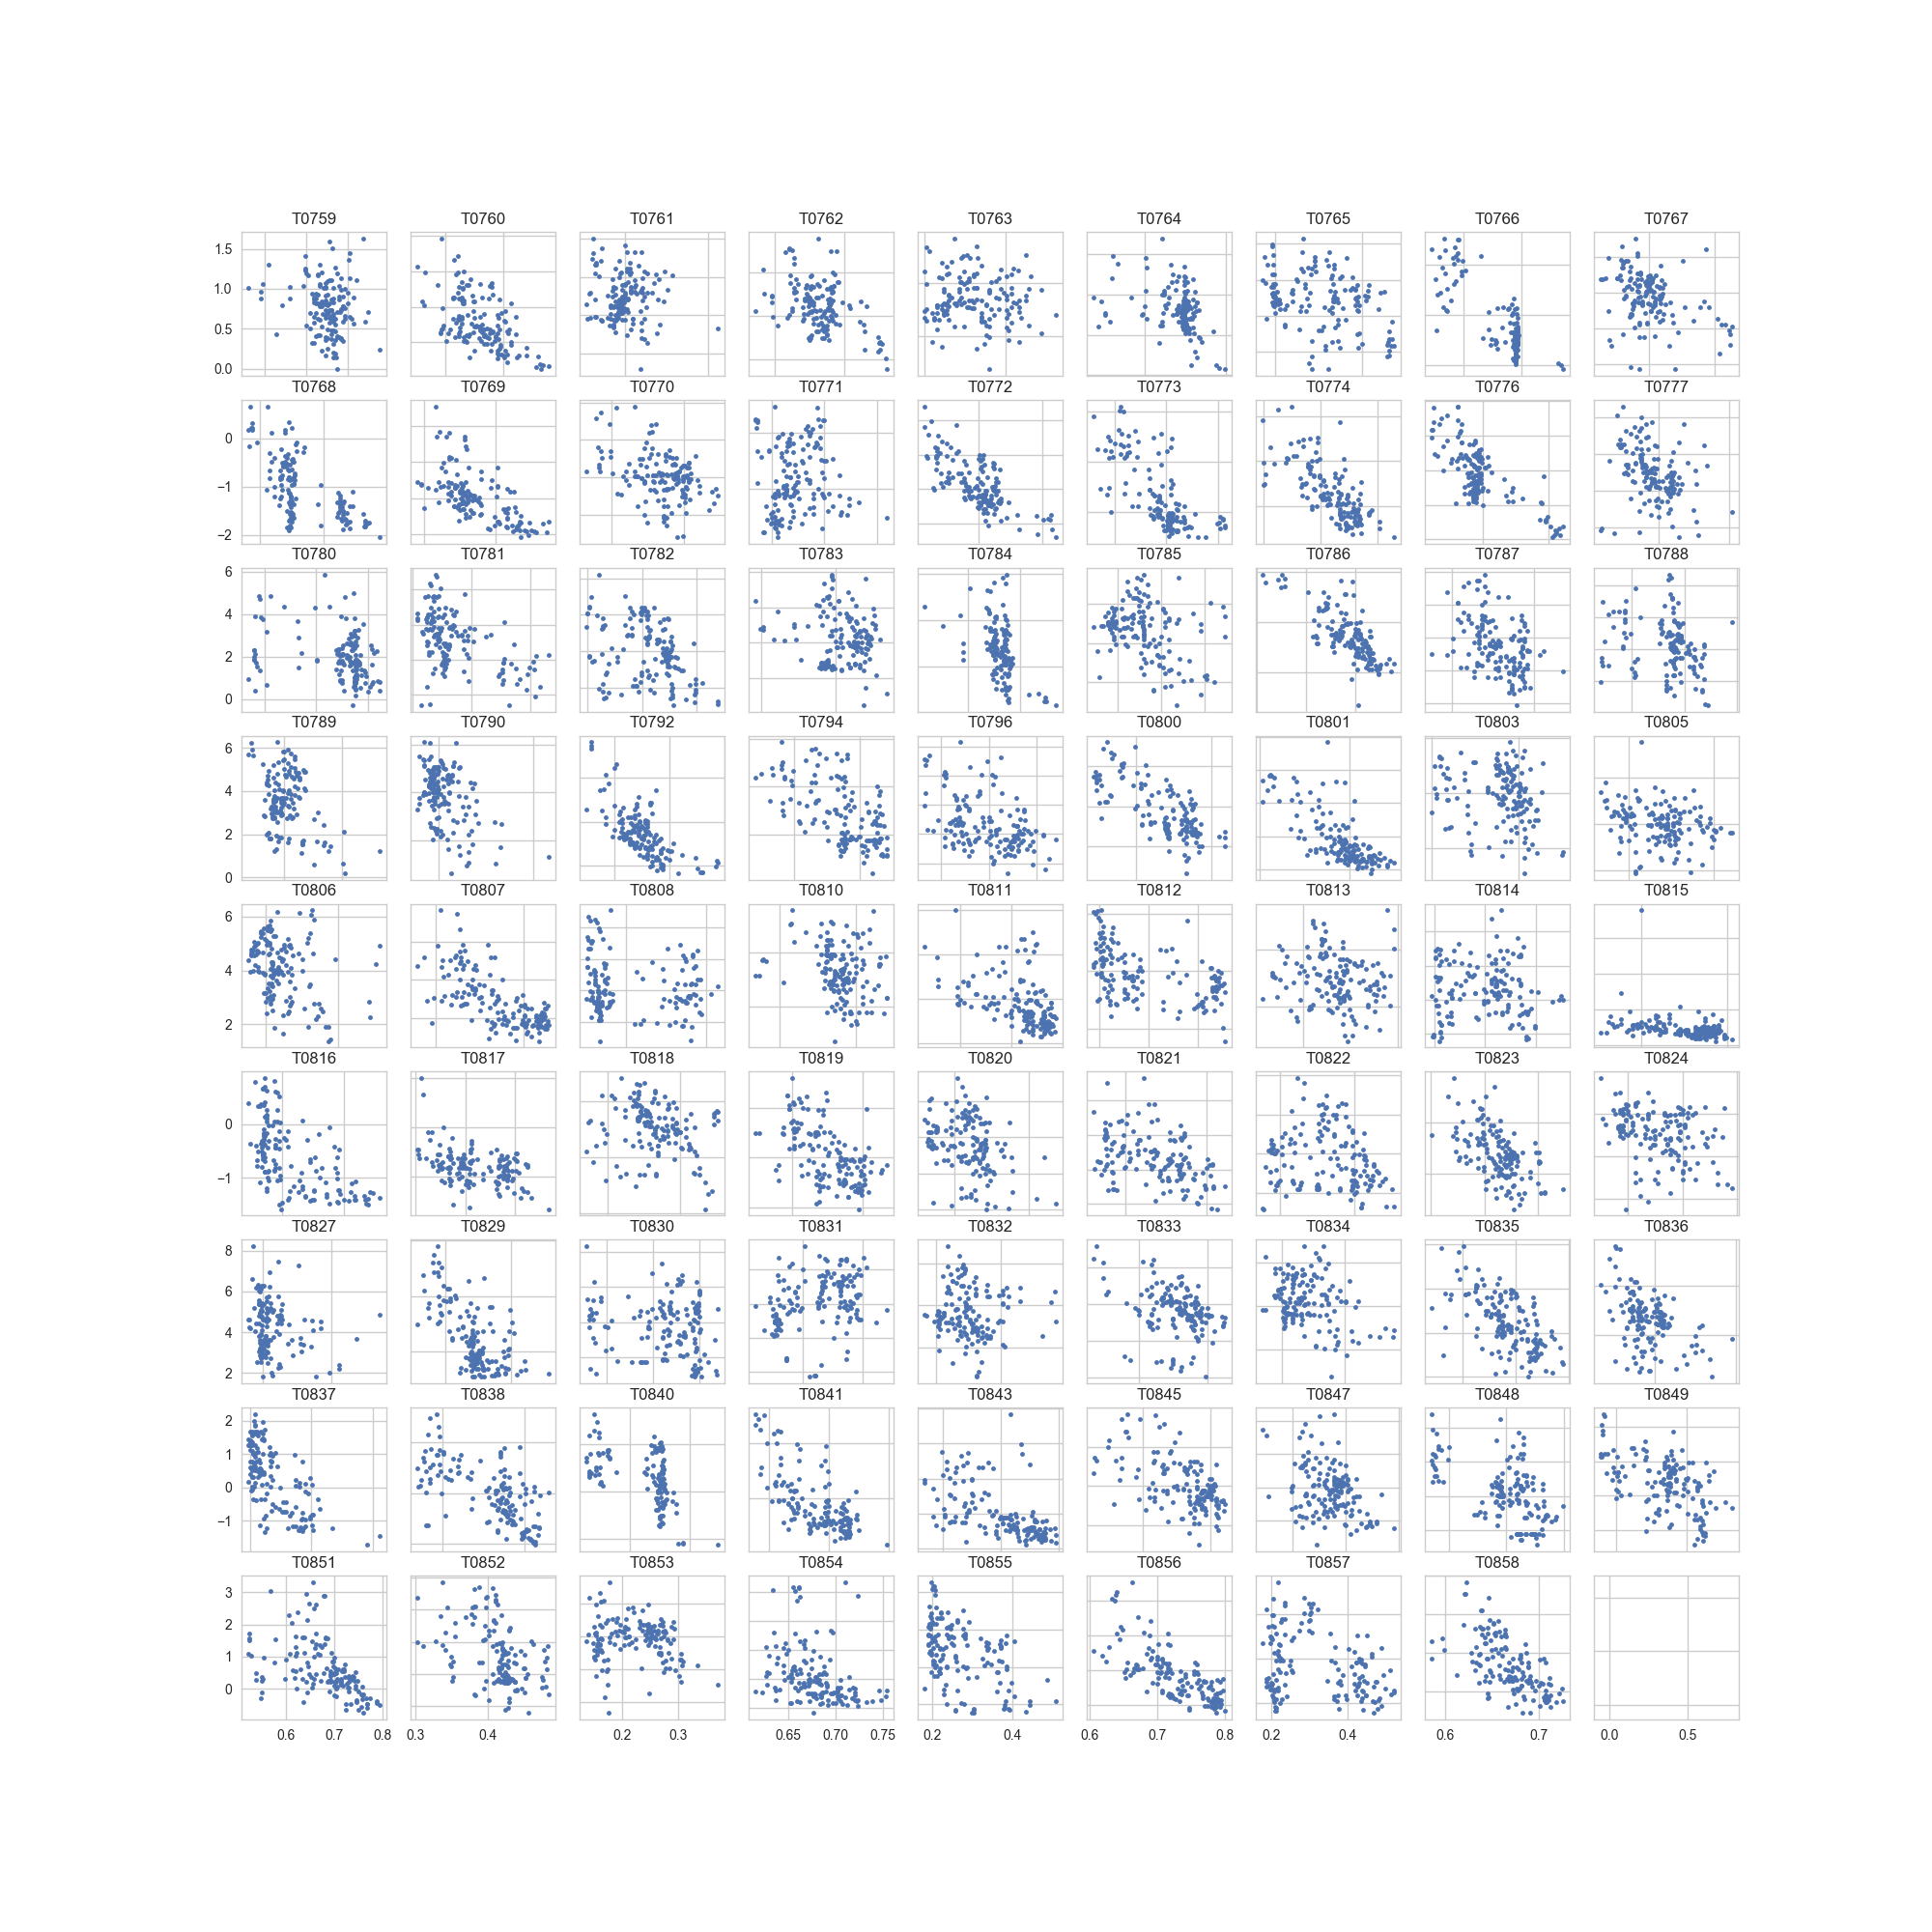
\includegraphics[width=0.9\paperwidth]{Fig/CASP11Stage2_SCWRL_sFinal_funnels.png}
    \hskip\headheight
    }
    \caption{Scoring funnels on Stage 2 CASP11}
    \label{Fig:Satage2CASP11Funnels}
\end{figure}

\begin{figure}[H]
    \centerline{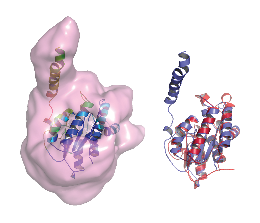
\includegraphics[width=0.8\linewidth]{Fig/FigT0776.eps}}
    \caption{Left: Output of the Grad-CAM analysis for layer 10 of
      the network projected on candidate structure Distill\_TS3 of
      target T0776. The isosurface shows the scaled outputs at the
      two-sigma level. The intensities of the outputs at the positions
      of the protein atoms are color-coded on the cartoon rendering of
      the structure, from blue (low intensity) to red (high
      intensity). Right: Cartoon representation of the Distill\_TS3
      decoy structure (in blue) aligned to the native structure (in
      red).}
    \label{Fig:GradCAMT0776}
\end{figure}



% \documentclass[letter,10pt]{article}
% \usepackage{graphicx}
% \usepackage{tabularx}
% \usepackage{ltxtable}
% \begin{document}	
\begin{center}
\makebox[0pt][c]{
\hskip-\footskip
\begin{tabularx}{0.9\paperwidth}{>{\raggedright}p{4.5cm}>{\raggedright}p{4.5cm}>{\raggedright}p{4.5cm}>{\raggedright\arraybackslash}p{4.5cm}}

				\hline
T0759 myprotein-me\_TS4 &T0759 BAKER-ROSETTASERVER\_TS4 &T0759 FFAS03\_TS1 &T0759 Seok-server\_TS2 \\
GDT\_TS = 0.25 &GDT\_TS = 0.31 &GDT\_TS = 0.34 &GDT\_TS = 0.36 \\
\begin{minipage}{\linewidth}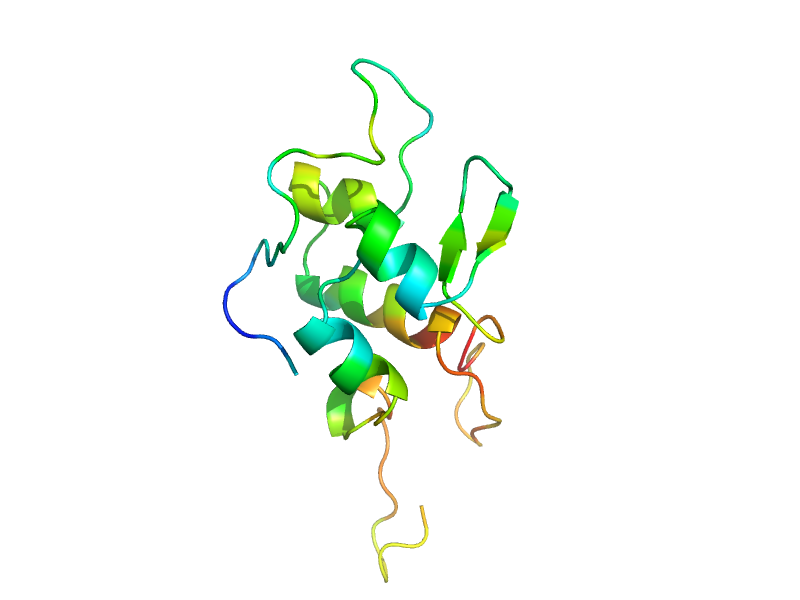
\includegraphics[width=\linewidth]{GradCAMOutput/T0759/T0759_myprotein-me_TS4.png}\end{minipage}&\begin{minipage}{\linewidth}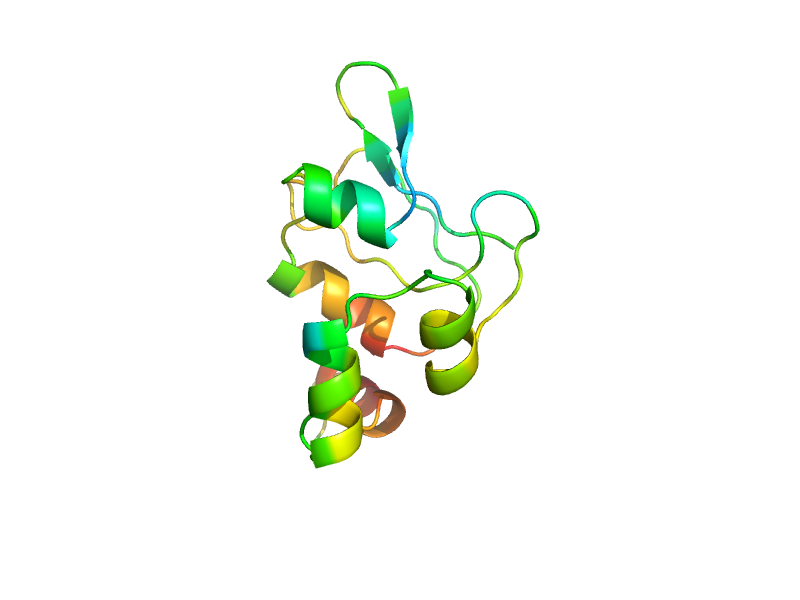
\includegraphics[width=\linewidth]{GradCAMOutput/T0759/T0759_BAKER-ROSETTASERVER_TS4.png}\end{minipage}&\begin{minipage}{\linewidth}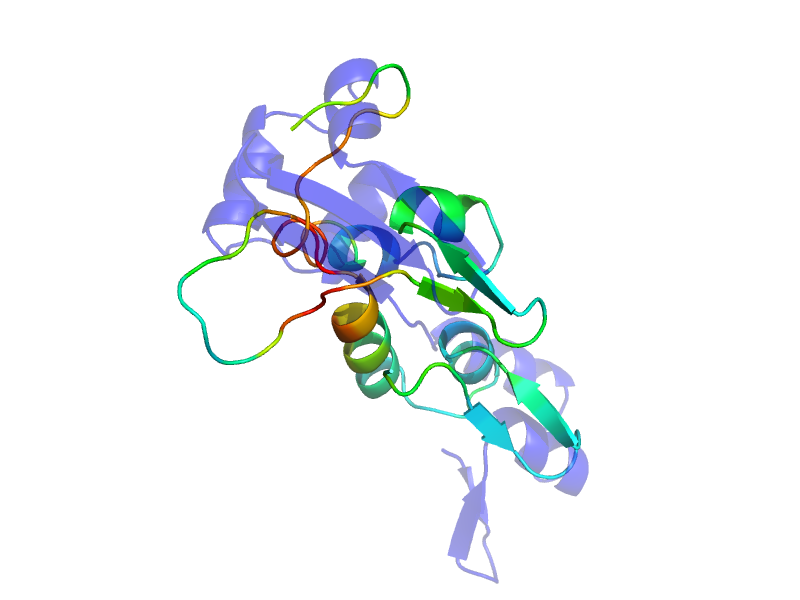
\includegraphics[width=\linewidth]{GradCAMOutput/T0759/T0759_FFAS03_TS1.png}\end{minipage}&\begin{minipage}{\linewidth}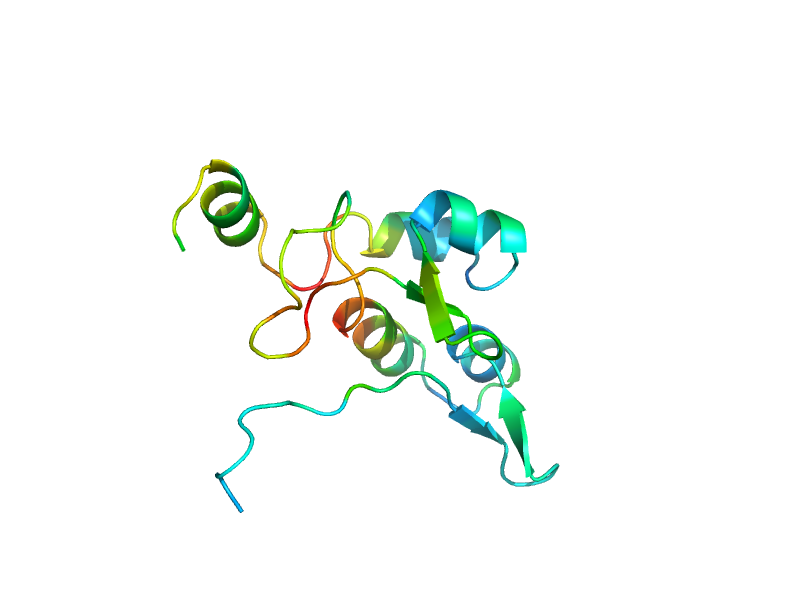
\includegraphics[width=\linewidth]{GradCAMOutput/T0759/T0759_Seok-server_TS2.png}\end{minipage}\\
\hline
T0760 FALCON\_MANUAL\_TS2 &T0760 Seok-server\_TS2 &T0760 MULTICOM-CONSTRUCT\_TS1 &T0760 FFAS03\_TS1 \\
GDT\_TS = 0.49 &GDT\_TS = 0.55 &GDT\_TS = 0.60 &GDT\_TS = 0.62 \\
\begin{minipage}{\linewidth}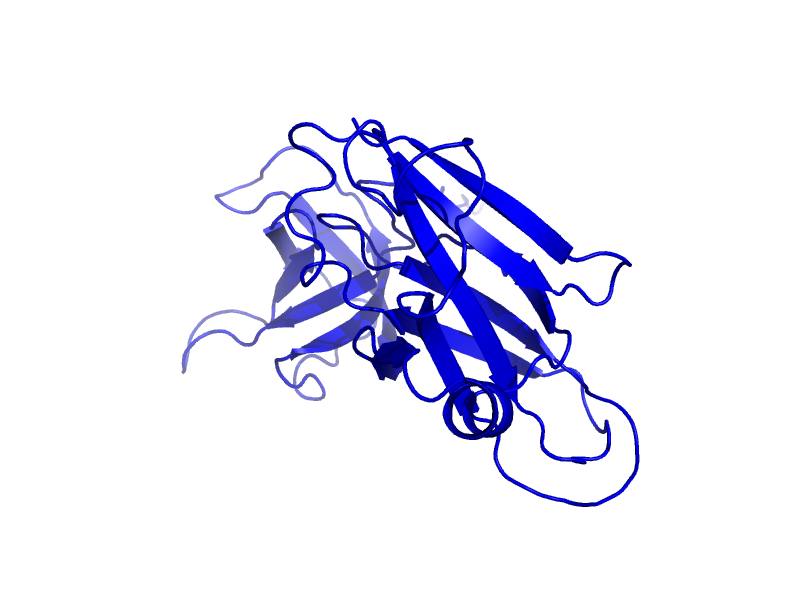
\includegraphics[width=\linewidth]{GradCAMOutput/T0760/T0760_FALCON_MANUAL_TS2.png}\end{minipage}&\begin{minipage}{\linewidth}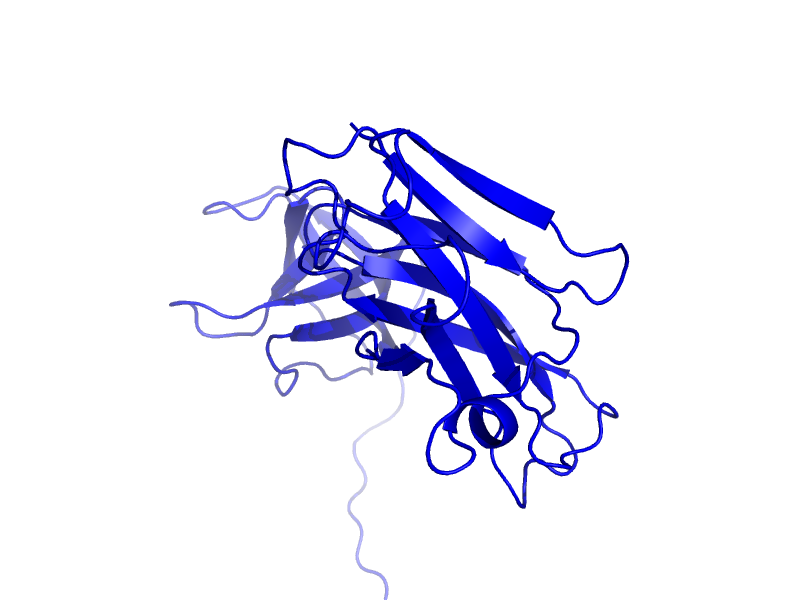
\includegraphics[width=\linewidth]{GradCAMOutput/T0760/T0760_Seok-server_TS2.png}\end{minipage}&\begin{minipage}{\linewidth}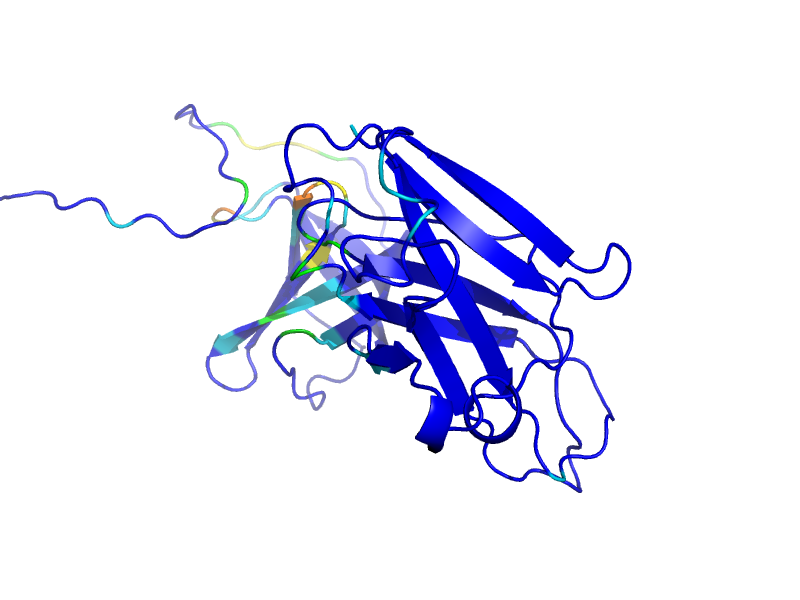
\includegraphics[width=\linewidth]{GradCAMOutput/T0760/T0760_MULTICOM-CONSTRUCT_TS1.png}\end{minipage}&\begin{minipage}{\linewidth}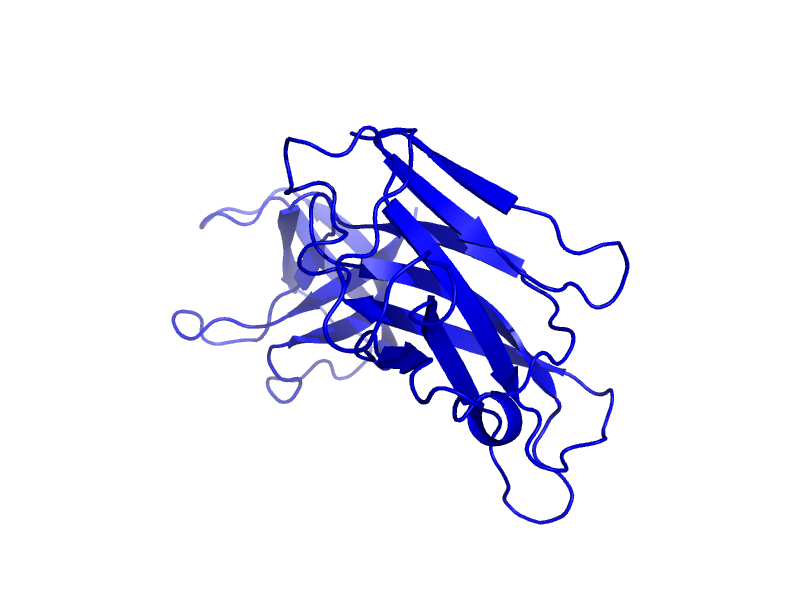
\includegraphics[width=\linewidth]{GradCAMOutput/T0760/T0760_FFAS03_TS1.png}\end{minipage}\\
\hline
T0761 MULTICOM-CONSTRUCT\_TS1 &T0761 RBO\_Aleph\_TS3 &T0761 RBO\_Aleph\_TS4 &T0761 BAKER-ROSETTASERVER\_TS4 \\
GDT\_TS = 0.09 &GDT\_TS = 0.10 &GDT\_TS = 0.12 &GDT\_TS = 0.16 \\
\begin{minipage}{\linewidth}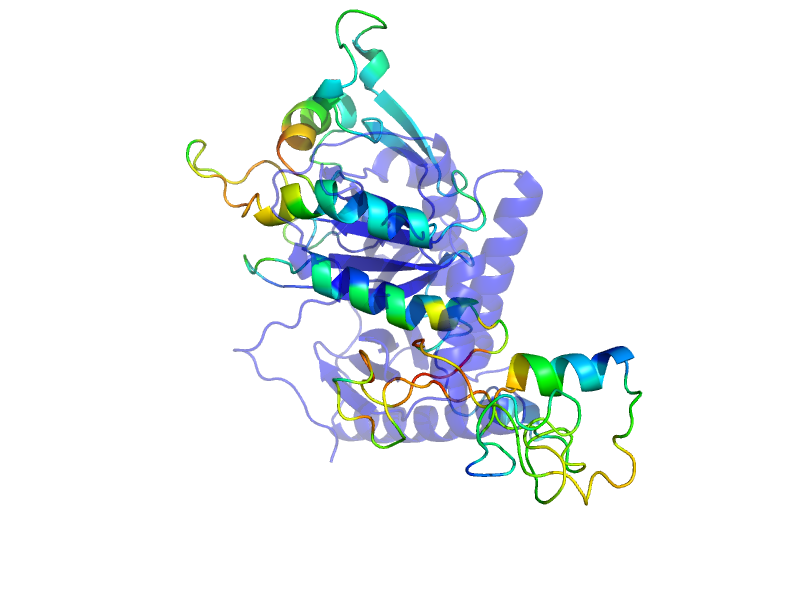
\includegraphics[width=\linewidth]{GradCAMOutput/T0761/T0761_MULTICOM-CONSTRUCT_TS1.png}\end{minipage}&\begin{minipage}{\linewidth}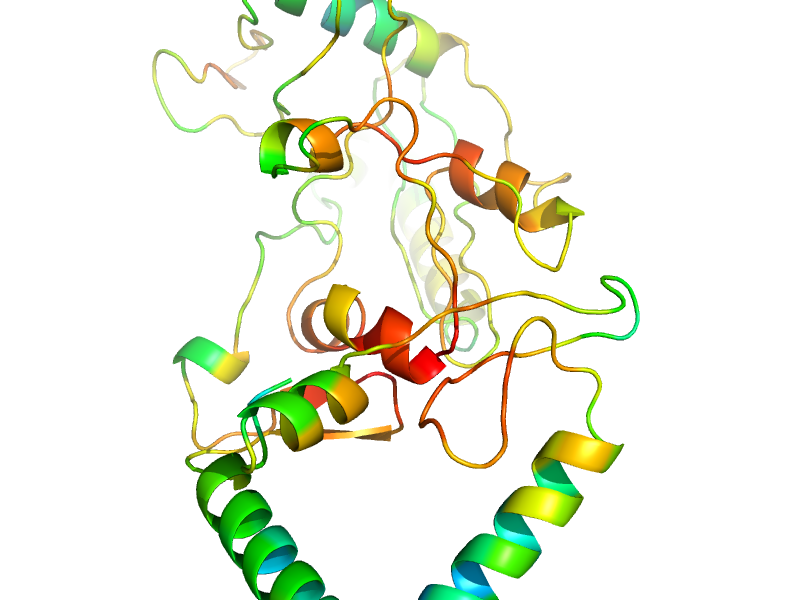
\includegraphics[width=\linewidth]{GradCAMOutput/T0761/T0761_RBO_Aleph_TS3.png}\end{minipage}&\begin{minipage}{\linewidth}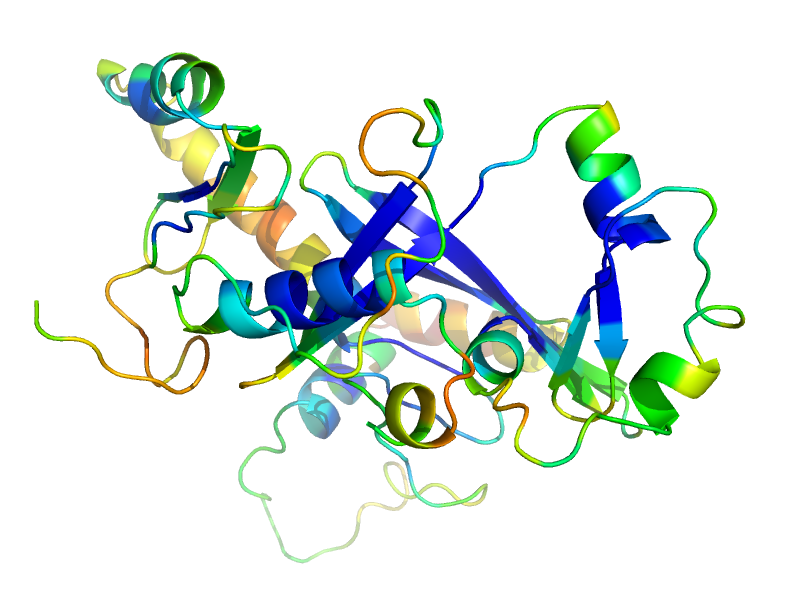
\includegraphics[width=\linewidth]{GradCAMOutput/T0761/T0761_RBO_Aleph_TS4.png}\end{minipage}&\begin{minipage}{\linewidth}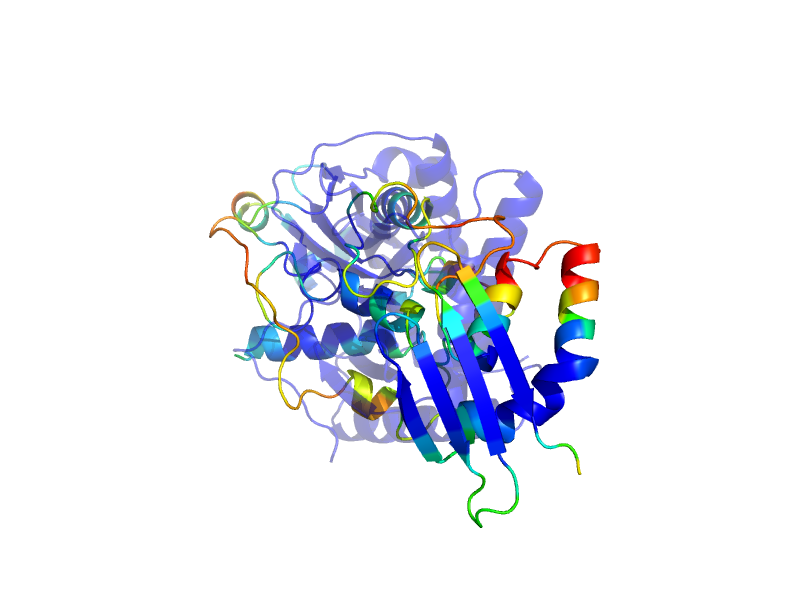
\includegraphics[width=\linewidth]{GradCAMOutput/T0761/T0761_BAKER-ROSETTASERVER_TS4.png}\end{minipage}\\
\hline
T0762 BhageerathH\_TS4 &T0762 RBO\_Aleph\_TS3 &T0762 MULTICOM-CONSTRUCT\_TS1 &T0762 FFAS03\_TS1 \\
GDT\_TS = 0.70 &GDT\_TS = 0.76 &GDT\_TS = 0.79 &GDT\_TS = 0.83 \\
\begin{minipage}{\linewidth}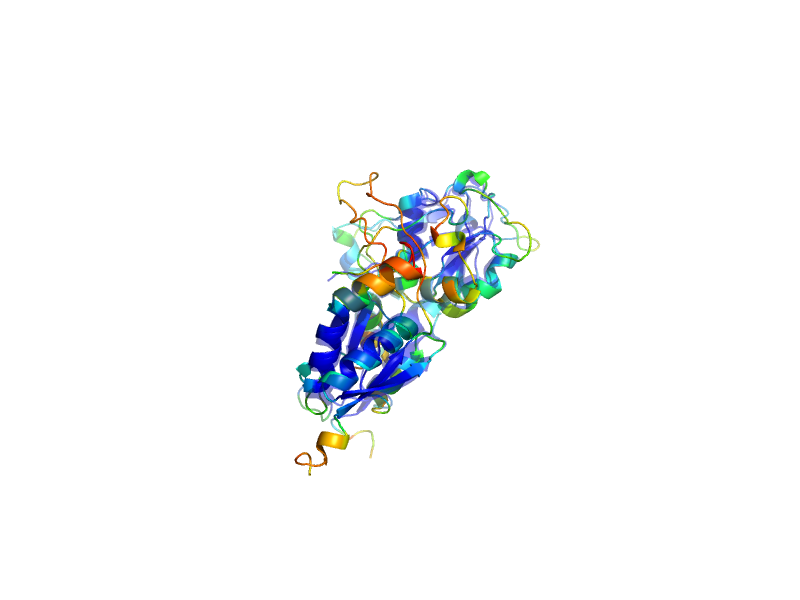
\includegraphics[width=\linewidth]{GradCAMOutput/T0762/T0762_BhageerathH_TS4.png}\end{minipage}&\begin{minipage}{\linewidth}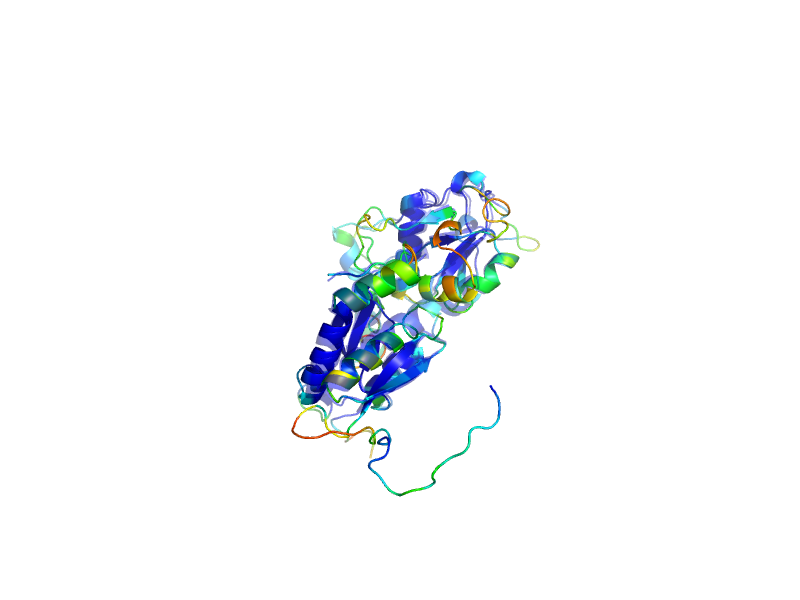
\includegraphics[width=\linewidth]{GradCAMOutput/T0762/T0762_RBO_Aleph_TS3.png}\end{minipage}&\begin{minipage}{\linewidth}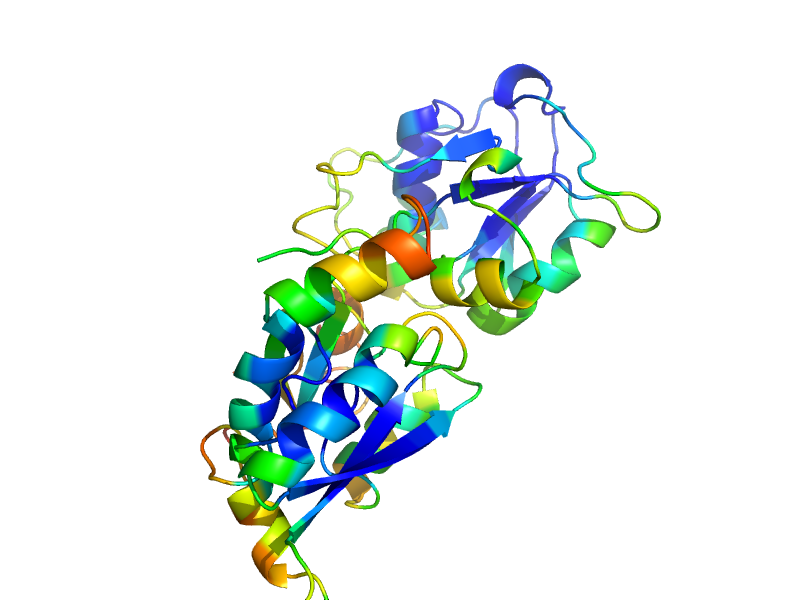
\includegraphics[width=\linewidth]{GradCAMOutput/T0762/T0762_MULTICOM-CONSTRUCT_TS1.png}\end{minipage}&\begin{minipage}{\linewidth}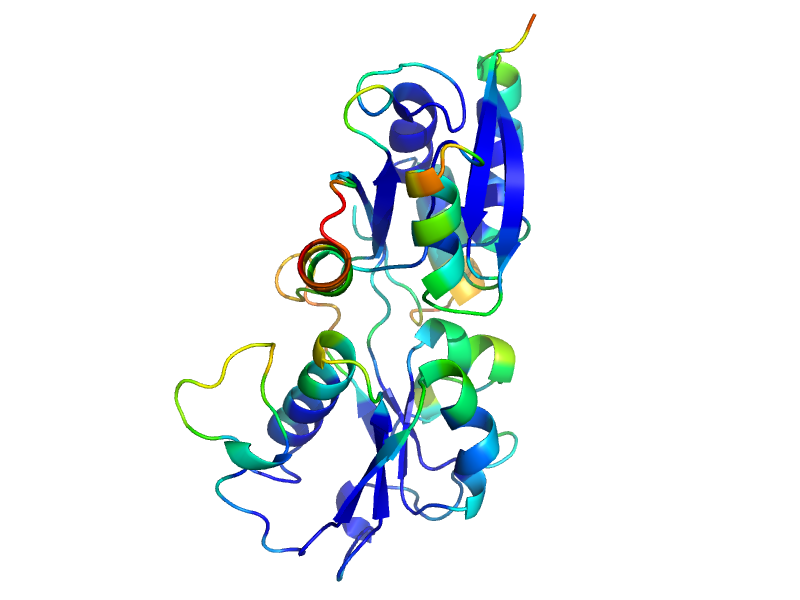
\includegraphics[width=\linewidth]{GradCAMOutput/T0762/T0762_FFAS03_TS1.png}\end{minipage}\\

\end{tabularx}
%}
\hskip\headheight}
\end{center}	
\begin{center}
\makebox[0pt][c]{
\hskip-\footskip
\begin{tabularx}{0.9\paperwidth}{X*{4}{p{4.5cm}}}

				\hline
T0763 FALCON\_MANUAL\_TS2 &T0763 Distill\_TS3 &T0763 RBO\_Aleph\_TS3 &T0763 MULTICOM-CONSTRUCT\_TS1 \\
GDT\_TS = 0.12 &GDT\_TS = 0.13 &GDT\_TS = 0.15 &GDT\_TS = 0.17 \\
\begin{minipage}{\linewidth}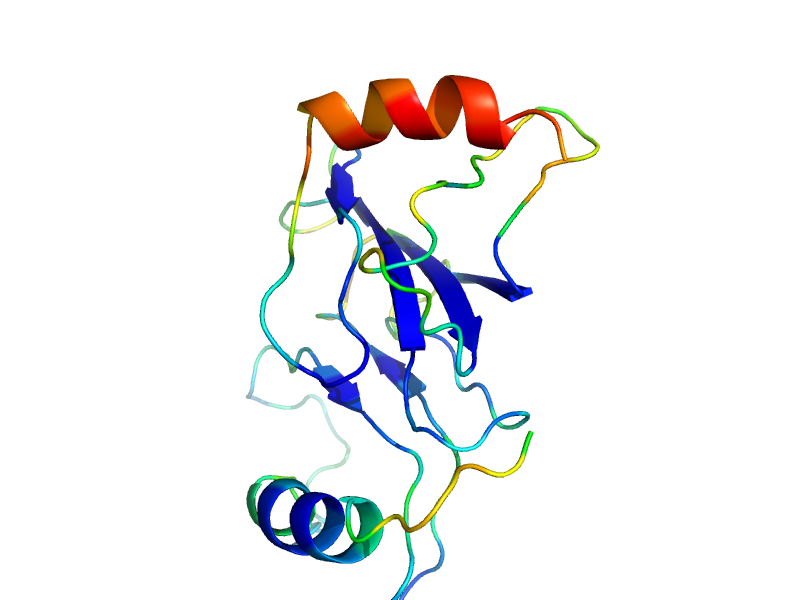
\includegraphics[width=\linewidth]{GradCAMOutput/T0763/T0763_FALCON_MANUAL_TS2.png}\end{minipage}&\begin{minipage}{\linewidth}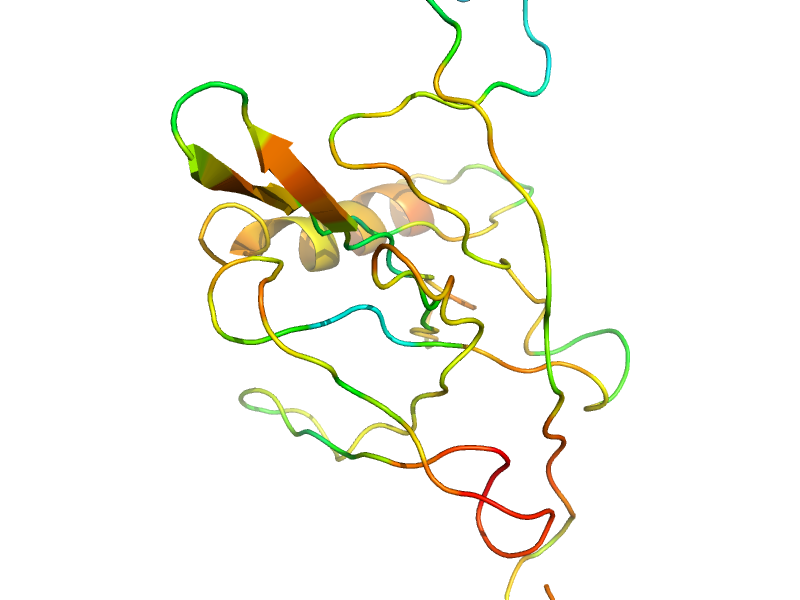
\includegraphics[width=\linewidth]{GradCAMOutput/T0763/T0763_Distill_TS3.png}\end{minipage}&\begin{minipage}{\linewidth}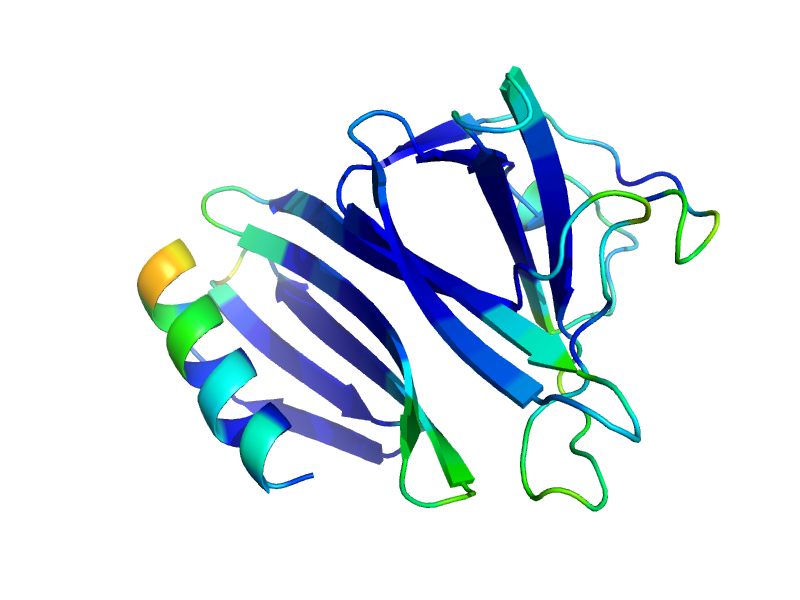
\includegraphics[width=\linewidth]{GradCAMOutput/T0763/T0763_RBO_Aleph_TS3.png}\end{minipage}&\begin{minipage}{\linewidth}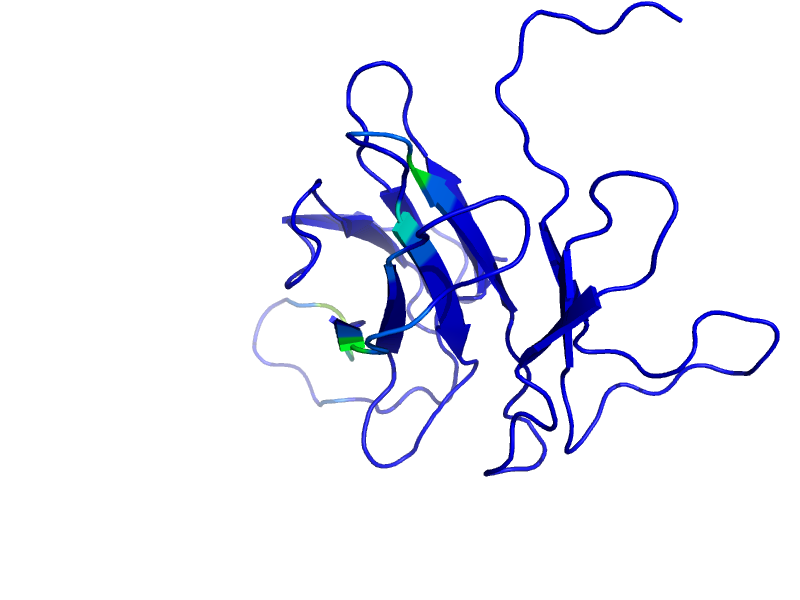
\includegraphics[width=\linewidth]{GradCAMOutput/T0763/T0763_MULTICOM-CONSTRUCT_TS1.png}\end{minipage}\\
\hline
T0764 RBO\_Aleph\_TS4 &T0764 BioShell-server\_TS3 &T0764 FFAS03\_TS1 &T0764 MUFOLD-Server\_TS4 \\
GDT\_TS = 0.50 &GDT\_TS = 0.60 &GDT\_TS = 0.65 &GDT\_TS = 0.72 \\
\begin{minipage}{\linewidth}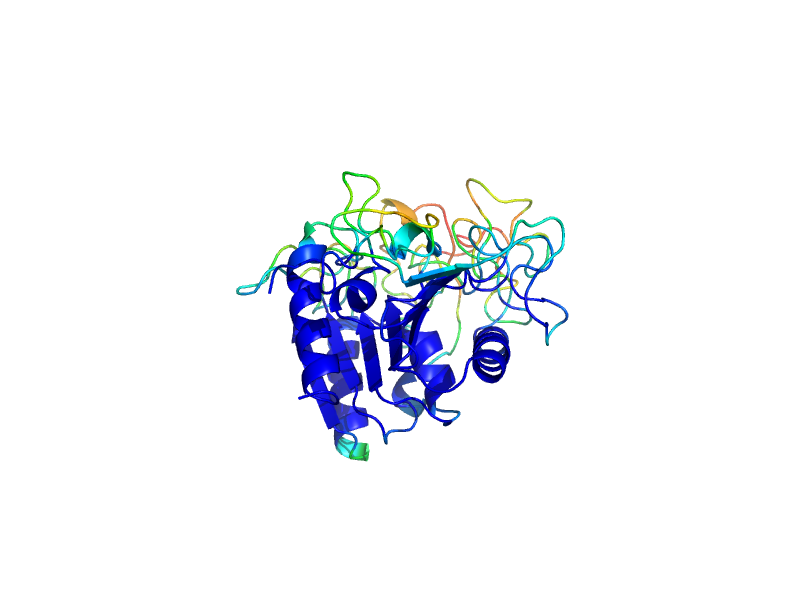
\includegraphics[width=\linewidth]{GradCAMOutput/T0764/T0764_RBO_Aleph_TS4.png}\end{minipage}&\begin{minipage}{\linewidth}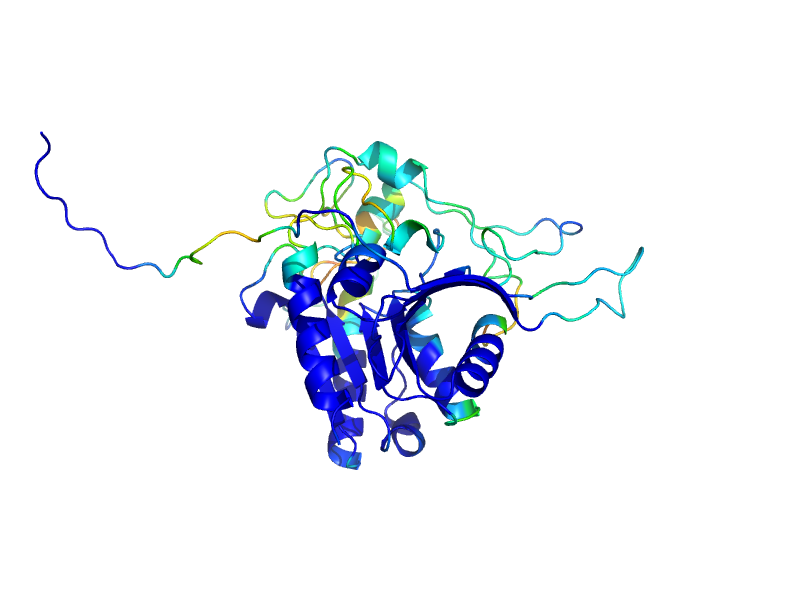
\includegraphics[width=\linewidth]{GradCAMOutput/T0764/T0764_BioShell-server_TS3.png}\end{minipage}&\begin{minipage}{\linewidth}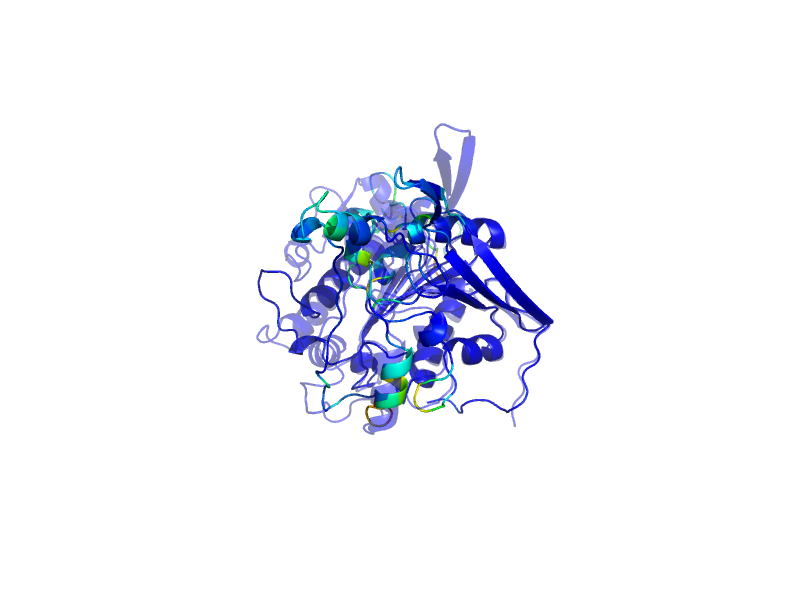
\includegraphics[width=\linewidth]{GradCAMOutput/T0764/T0764_FFAS03_TS1.png}\end{minipage}&\begin{minipage}{\linewidth}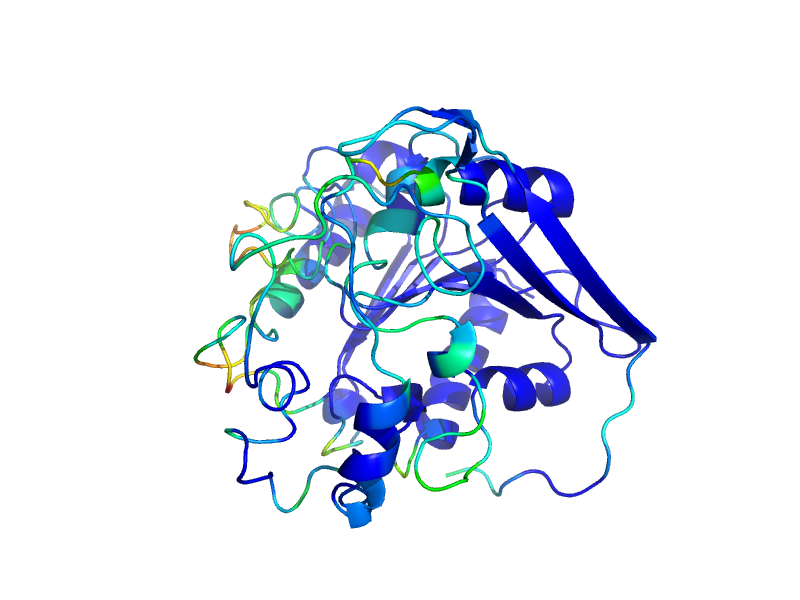
\includegraphics[width=\linewidth]{GradCAMOutput/T0764/T0764_MUFOLD-Server_TS4.png}\end{minipage}\\
\hline
T0765 MUFOLD-Server\_TS4 &T0765 RBO\_Aleph\_TS3 &T0765 Distill\_TS3 &T0765 MULTICOM-CONSTRUCT\_TS1 \\
GDT\_TS = 0.19 &GDT\_TS = 0.31 &GDT\_TS = 0.39 &GDT\_TS = 0.42 \\
\begin{minipage}{\linewidth}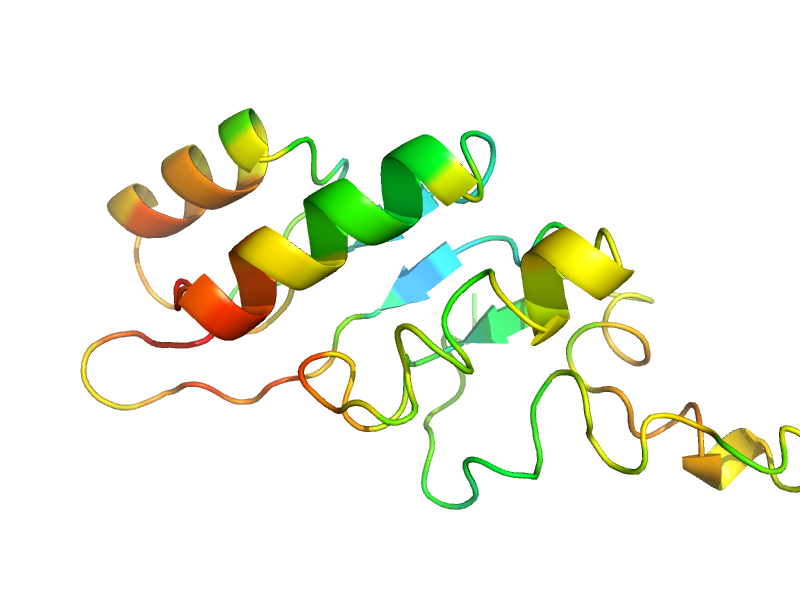
\includegraphics[width=\linewidth]{GradCAMOutput/T0765/T0765_MUFOLD-Server_TS4.png}\end{minipage}&\begin{minipage}{\linewidth}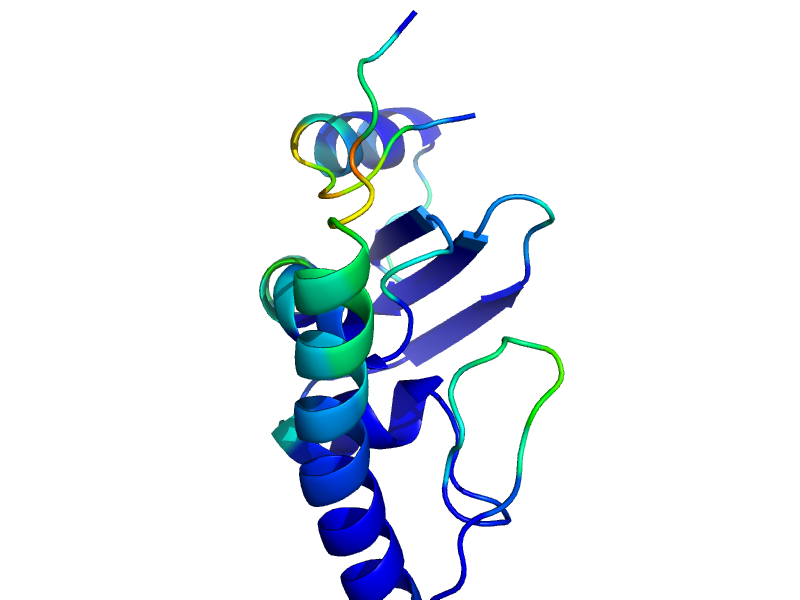
\includegraphics[width=\linewidth]{GradCAMOutput/T0765/T0765_RBO_Aleph_TS3.png}\end{minipage}&\begin{minipage}{\linewidth}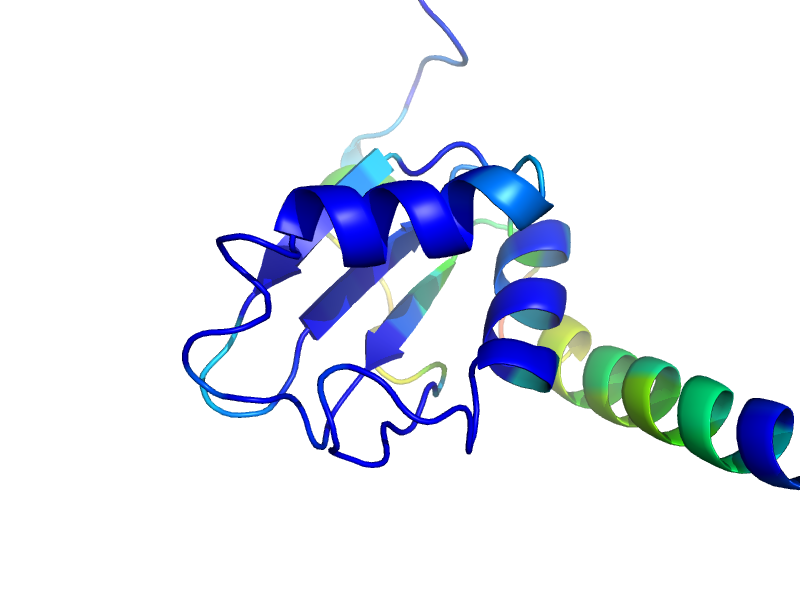
\includegraphics[width=\linewidth]{GradCAMOutput/T0765/T0765_Distill_TS3.png}\end{minipage}&\begin{minipage}{\linewidth}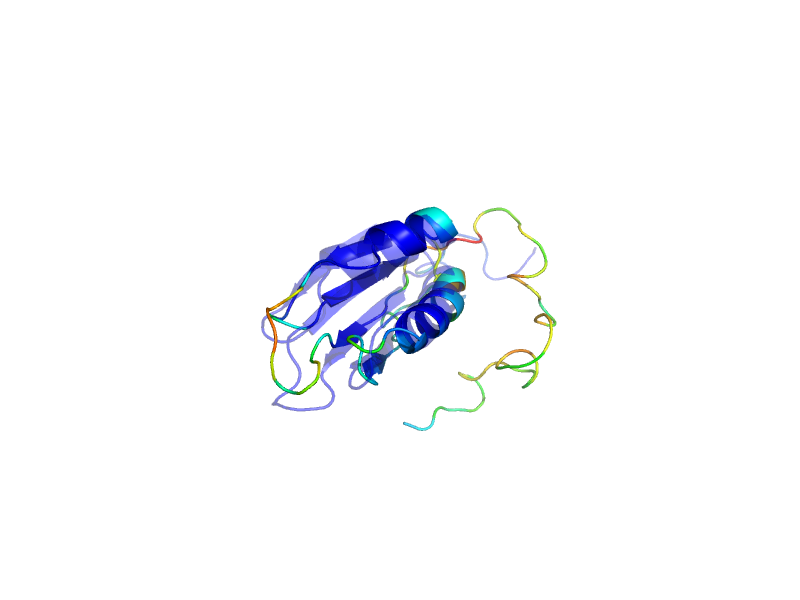
\includegraphics[width=\linewidth]{GradCAMOutput/T0765/T0765_MULTICOM-CONSTRUCT_TS1.png}\end{minipage}\\
\hline
T0766 RBO\_Aleph\_TS3 &T0766 TASSER-VMT\_TS2 &T0766 MULTICOM-CONSTRUCT\_TS1 &T0766 FFAS03\_TS1 \\
GDT\_TS = 0.53 &GDT\_TS = 0.67 &GDT\_TS = 0.78 &GDT\_TS = 0.94 \\
\begin{minipage}{\linewidth}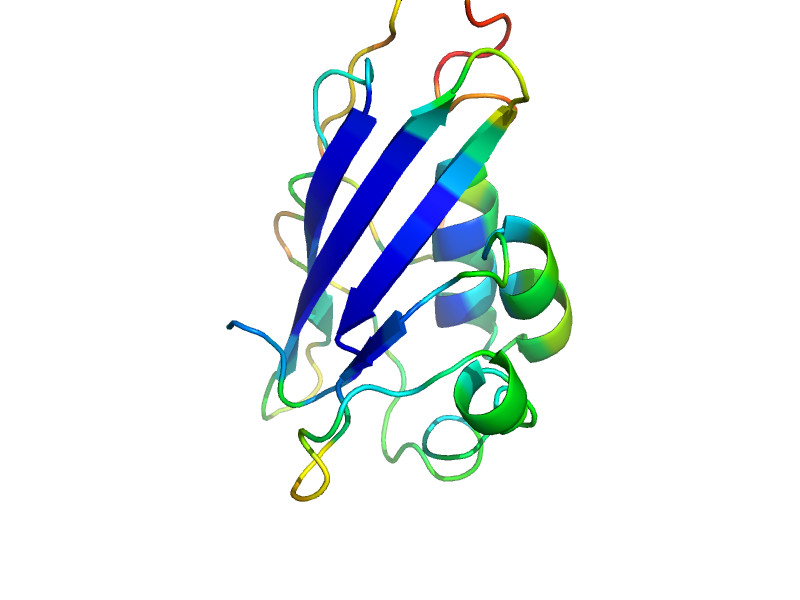
\includegraphics[width=\linewidth]{GradCAMOutput/T0766/T0766_RBO_Aleph_TS3.png}\end{minipage}&\begin{minipage}{\linewidth}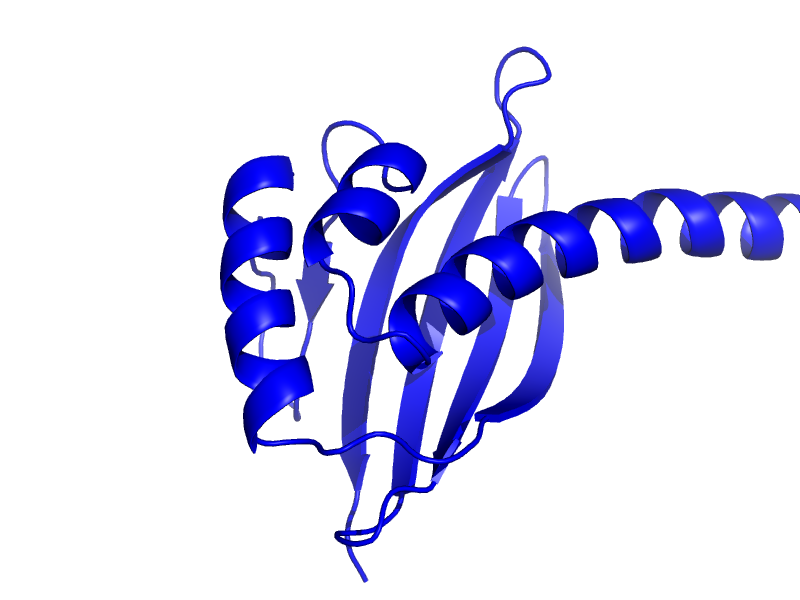
\includegraphics[width=\linewidth]{GradCAMOutput/T0766/T0766_TASSER-VMT_TS2.png}\end{minipage}&\begin{minipage}{\linewidth}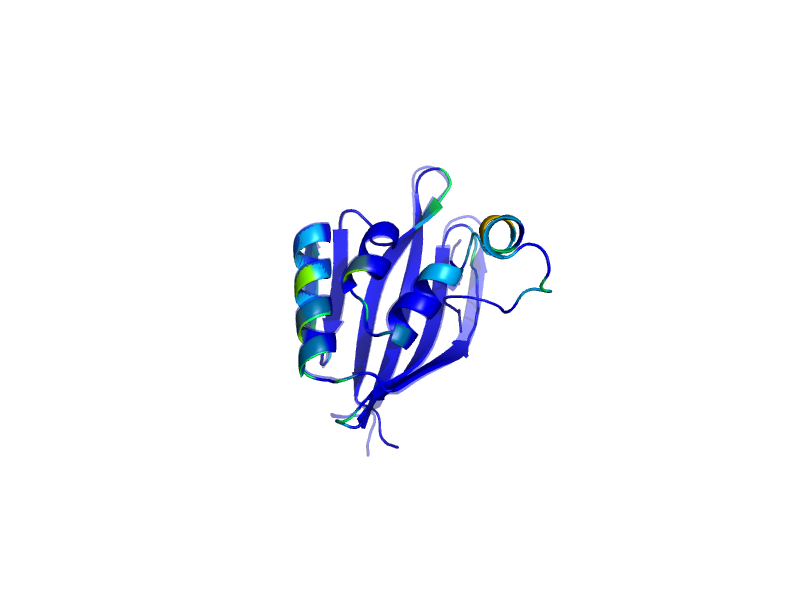
\includegraphics[width=\linewidth]{GradCAMOutput/T0766/T0766_MULTICOM-CONSTRUCT_TS1.png}\end{minipage}&\begin{minipage}{\linewidth}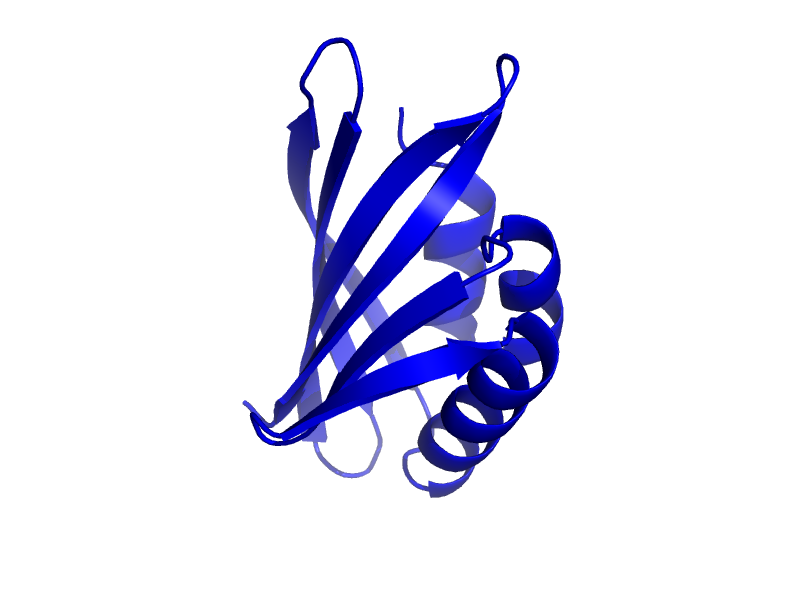
\includegraphics[width=\linewidth]{GradCAMOutput/T0766/T0766_FFAS03_TS1.png}\end{minipage}\\

\end{tabularx}
%}
\hskip\headheight}
\end{center}	
\begin{center}
\makebox[0pt][c]{
\hskip-\footskip
\begin{tabularx}{0.9\paperwidth}{X*{4}{p{4.5cm}}}

				\hline
T0767 BioShell-server\_TS3 &T0767 MULTICOM-CONSTRUCT\_TS1 &T0767 Pcons-net\_TS1 &T0767 RBO\_Aleph\_TS3 \\
GDT\_TS = 0.08 &GDT\_TS = 0.09 &GDT\_TS = 0.12 &GDT\_TS = 0.15 \\
\begin{minipage}{\linewidth}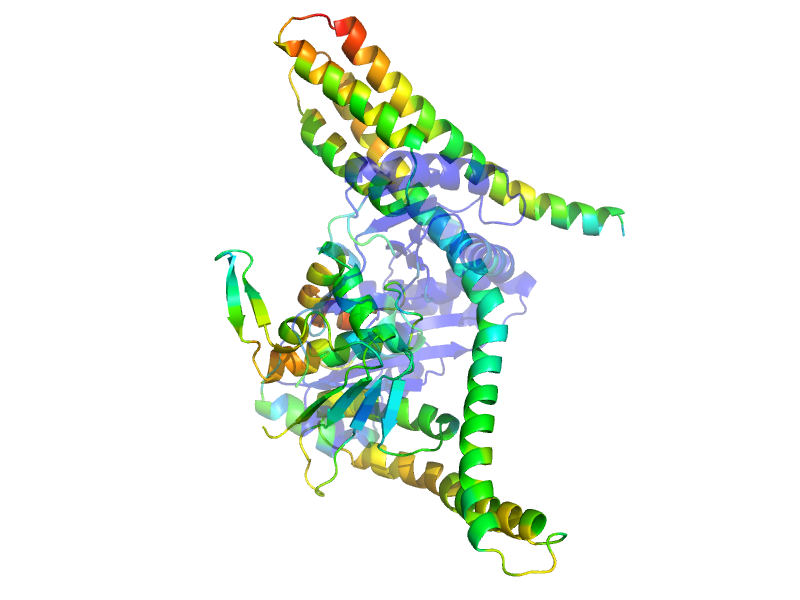
\includegraphics[width=\linewidth]{GradCAMOutput/T0767/T0767_BioShell-server_TS3.png}\end{minipage}&\begin{minipage}{\linewidth}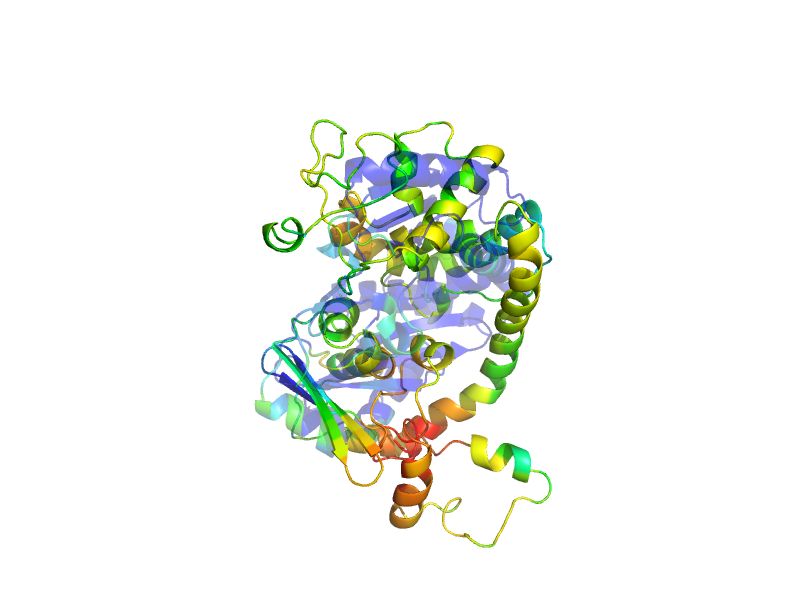
\includegraphics[width=\linewidth]{GradCAMOutput/T0767/T0767_MULTICOM-CONSTRUCT_TS1.png}\end{minipage}&\begin{minipage}{\linewidth}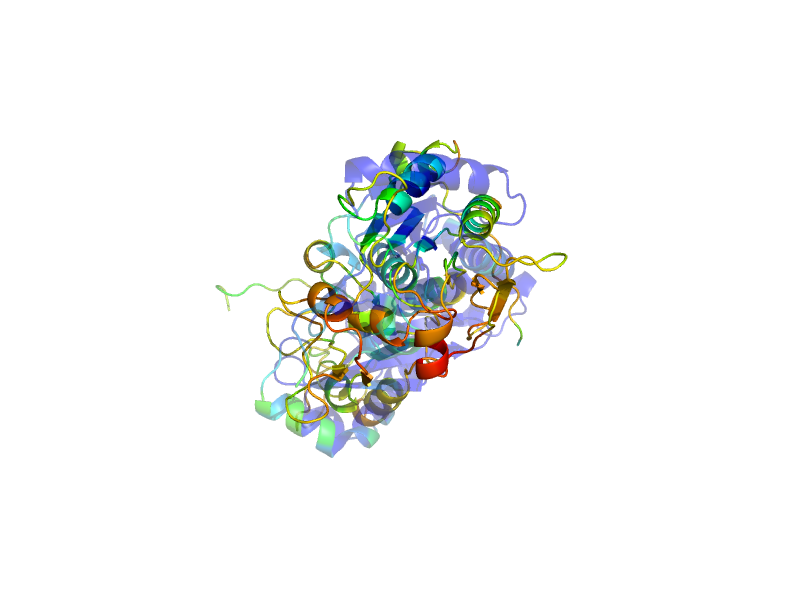
\includegraphics[width=\linewidth]{GradCAMOutput/T0767/T0767_Pcons-net_TS1.png}\end{minipage}&\begin{minipage}{\linewidth}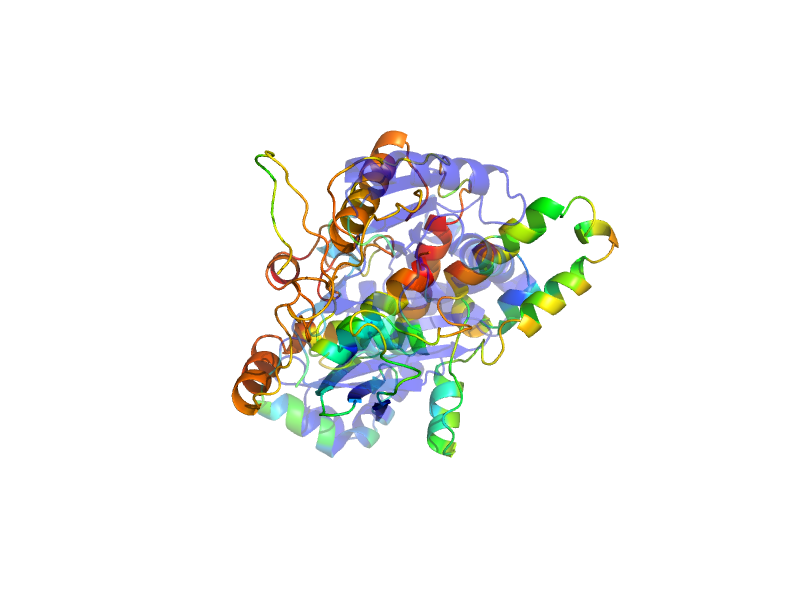
\includegraphics[width=\linewidth]{GradCAMOutput/T0767/T0767_RBO_Aleph_TS3.png}\end{minipage}\\
\hline
T0768 Distill\_TS3 &T0768 FFAS03\_TS1 &T0768 FALCON\_MANUAL\_TS2 &T0768 nns\_TS5 \\
GDT\_TS = 0.37 &GDT\_TS = 0.49 &GDT\_TS = 0.65 &GDT\_TS = 0.68 \\
\begin{minipage}{\linewidth}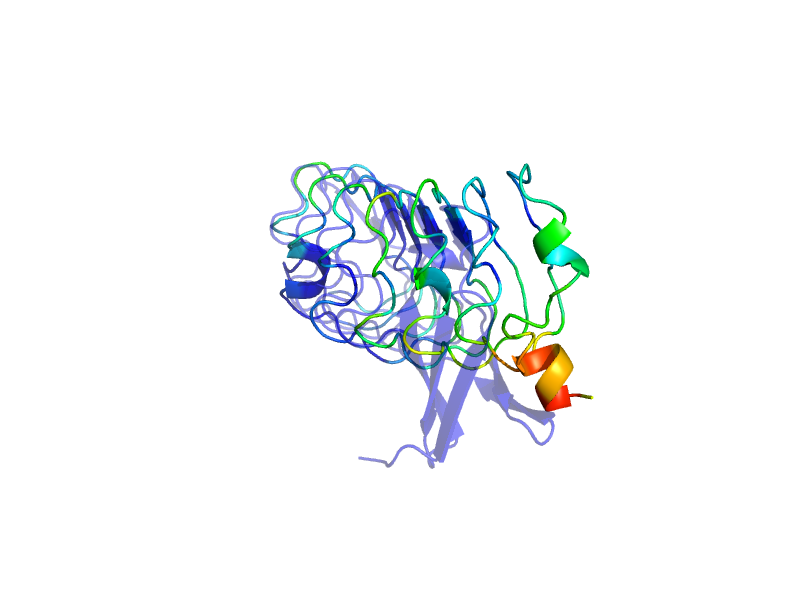
\includegraphics[width=\linewidth]{GradCAMOutput/T0768/T0768_Distill_TS3.png}\end{minipage}&\begin{minipage}{\linewidth}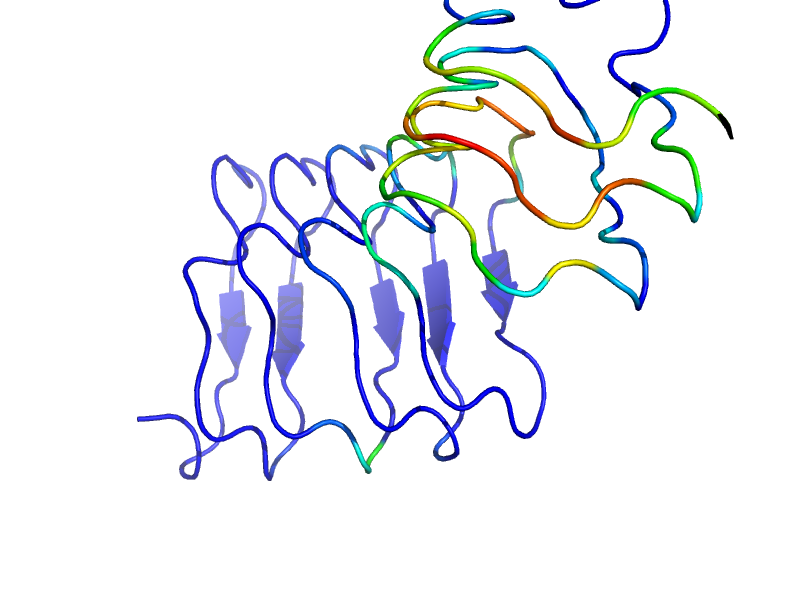
\includegraphics[width=\linewidth]{GradCAMOutput/T0768/T0768_FFAS03_TS1.png}\end{minipage}&\begin{minipage}{\linewidth}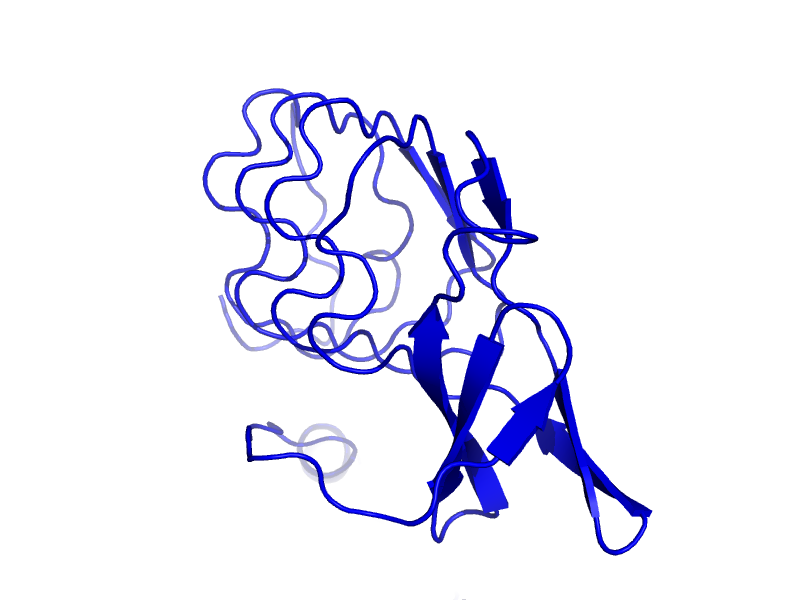
\includegraphics[width=\linewidth]{GradCAMOutput/T0768/T0768_FALCON_MANUAL_TS2.png}\end{minipage}&\begin{minipage}{\linewidth}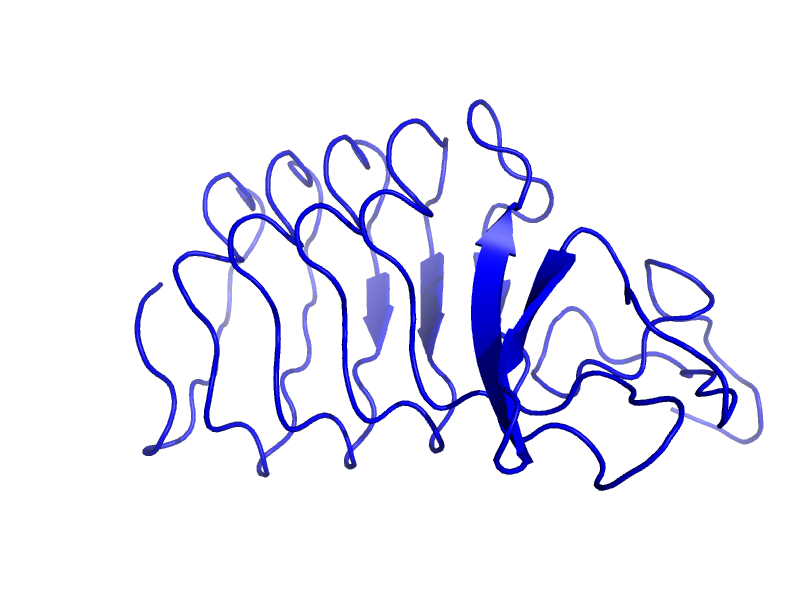
\includegraphics[width=\linewidth]{GradCAMOutput/T0768/T0768_nns_TS5.png}\end{minipage}\\
\hline
T0769 MUFOLD-Server\_TS4 &T0769 MULTICOM-CONSTRUCT\_TS1 &T0769 RBO\_Aleph\_TS3 &T0769 BAKER-ROSETTASERVER\_TS4 \\
GDT\_TS = 0.44 &GDT\_TS = 0.48 &GDT\_TS = 0.66 &GDT\_TS = 0.68 \\
\begin{minipage}{\linewidth}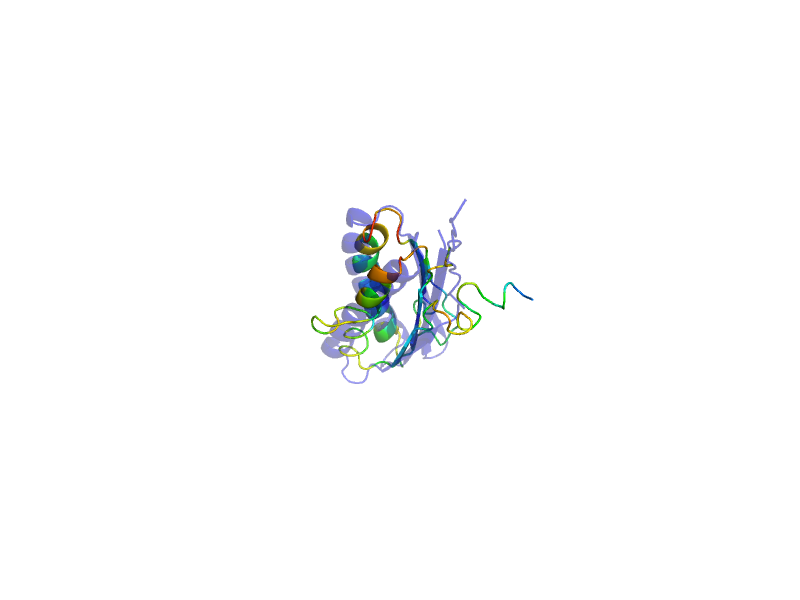
\includegraphics[width=\linewidth]{GradCAMOutput/T0769/T0769_MUFOLD-Server_TS4.png}\end{minipage}&\begin{minipage}{\linewidth}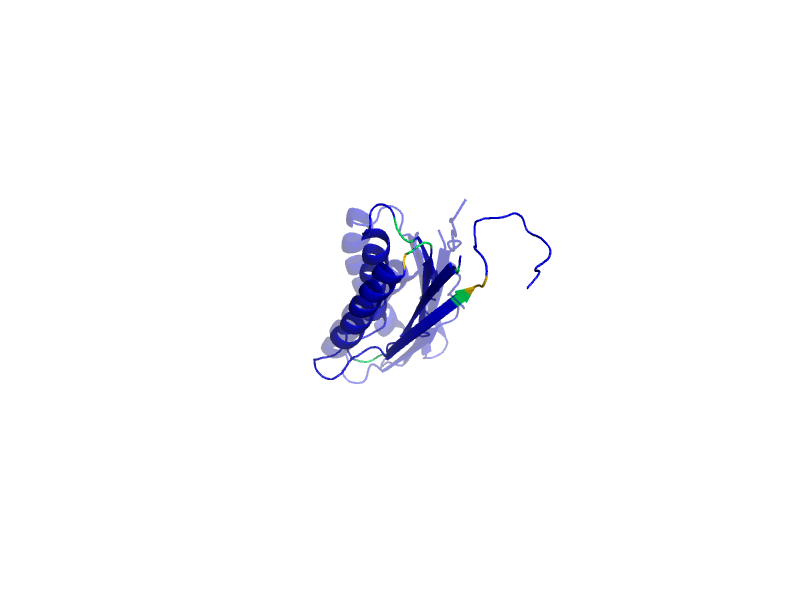
\includegraphics[width=\linewidth]{GradCAMOutput/T0769/T0769_MULTICOM-CONSTRUCT_TS1.png}\end{minipage}&\begin{minipage}{\linewidth}\includegraphics[width=\linewidth]{GradCAMOutput/T0769/T0769_RBO_Aleph_TS3.png}\end{minipage}&\begin{minipage}{\linewidth}\includegraphics[width=\linewidth]{GradCAMOutput/T0769/T0769_BAKER-ROSETTASERVER_TS4.png}\end{minipage}\\
\hline
T0770 MUFOLD-Server\_TS4 &T0770 Distill\_TS3 &T0770 RBO\_Aleph\_TS3 &T0770 RBO\_Aleph\_TS4 \\
GDT\_TS = 0.48 &GDT\_TS = 0.55 &GDT\_TS = 0.60 &GDT\_TS = 0.62 \\
\begin{minipage}{\linewidth}\includegraphics[width=\linewidth]{GradCAMOutput/T0770/T0770_MUFOLD-Server_TS4.png}\end{minipage}&\begin{minipage}{\linewidth}\includegraphics[width=\linewidth]{GradCAMOutput/T0770/T0770_Distill_TS3.png}\end{minipage}&\begin{minipage}{\linewidth}\includegraphics[width=\linewidth]{GradCAMOutput/T0770/T0770_RBO_Aleph_TS3.png}\end{minipage}&\begin{minipage}{\linewidth}\includegraphics[width=\linewidth]{GradCAMOutput/T0770/T0770_RBO_Aleph_TS4.png}\end{minipage}\\

\end{tabularx}
%}
\hskip\headheight}
\end{center}	
\begin{center}
\makebox[0pt][c]{
\hskip-\footskip
\begin{tabularx}{0.9\paperwidth}{X*{4}{p{4.5cm}}}

				\hline
T0771 MULTICOM-CONSTRUCT\_TS1 &T0771 RBO\_Aleph\_TS3 &T0771 RBO\_Aleph\_TS4 &T0771 BAKER-ROSETTASERVER\_TS5 \\
GDT\_TS = 0.10 &GDT\_TS = 0.14 &GDT\_TS = 0.15 &GDT\_TS = 0.21 \\
\begin{minipage}{\linewidth}\includegraphics[width=\linewidth]{GradCAMOutput/T0771/T0771_MULTICOM-CONSTRUCT_TS1.png}\end{minipage}&\begin{minipage}{\linewidth}\includegraphics[width=\linewidth]{GradCAMOutput/T0771/T0771_RBO_Aleph_TS3.png}\end{minipage}&\begin{minipage}{\linewidth}\includegraphics[width=\linewidth]{GradCAMOutput/T0771/T0771_RBO_Aleph_TS4.png}\end{minipage}&\begin{minipage}{\linewidth}\includegraphics[width=\linewidth]{GradCAMOutput/T0771/T0771_BAKER-ROSETTASERVER_TS5.png}\end{minipage}\\
\hline
T0772 Distill\_TS3 &T0772 RBO\_Aleph\_TS3 &T0772 BAKER-ROSETTASERVER\_TS4 &T0772 FFAS03\_TS1 \\
GDT\_TS = 0.45 &GDT\_TS = 0.51 &GDT\_TS = 0.56 &GDT\_TS = 0.59 \\
\begin{minipage}{\linewidth}\includegraphics[width=\linewidth]{GradCAMOutput/T0772/T0772_Distill_TS3.png}\end{minipage}&\begin{minipage}{\linewidth}\includegraphics[width=\linewidth]{GradCAMOutput/T0772/T0772_RBO_Aleph_TS3.png}\end{minipage}&\begin{minipage}{\linewidth}\includegraphics[width=\linewidth]{GradCAMOutput/T0772/T0772_BAKER-ROSETTASERVER_TS4.png}\end{minipage}&\begin{minipage}{\linewidth}\includegraphics[width=\linewidth]{GradCAMOutput/T0772/T0772_FFAS03_TS1.png}\end{minipage}\\
\hline
T0773 eThread\_TS1 &T0773 MULTICOM-CLUSTER\_TS2 &T0773 MULTICOM-CONSTRUCT\_TS1 &T0773 RBO\_Aleph\_TS3 \\
GDT\_TS = 0.44 &GDT\_TS = 0.57 &GDT\_TS = 0.61 &GDT\_TS = 0.82 \\
\begin{minipage}{\linewidth}\includegraphics[width=\linewidth]{GradCAMOutput/T0773/T0773_eThread_TS1.png}\end{minipage}&\begin{minipage}{\linewidth}\includegraphics[width=\linewidth]{GradCAMOutput/T0773/T0773_MULTICOM-CLUSTER_TS2.png}\end{minipage}&\begin{minipage}{\linewidth}\includegraphics[width=\linewidth]{GradCAMOutput/T0773/T0773_MULTICOM-CONSTRUCT_TS1.png}\end{minipage}&\begin{minipage}{\linewidth}\includegraphics[width=\linewidth]{GradCAMOutput/T0773/T0773_RBO_Aleph_TS3.png}\end{minipage}\\
\hline
T0774 Seok-server\_TS4 &T0774 RBO\_Aleph\_TS3 &T0774 FFAS03\_TS1 &T0774 Atome2\_CBS\_TS3 \\
GDT\_TS = 0.20 &GDT\_TS = 0.27 &GDT\_TS = 0.33 &GDT\_TS = 0.43 \\
\begin{minipage}{\linewidth}\includegraphics[width=\linewidth]{GradCAMOutput/T0774/T0774_Seok-server_TS4.png}\end{minipage}&\begin{minipage}{\linewidth}\includegraphics[width=\linewidth]{GradCAMOutput/T0774/T0774_RBO_Aleph_TS3.png}\end{minipage}&\begin{minipage}{\linewidth}\includegraphics[width=\linewidth]{GradCAMOutput/T0774/T0774_FFAS03_TS1.png}\end{minipage}&\begin{minipage}{\linewidth}\includegraphics[width=\linewidth]{GradCAMOutput/T0774/T0774_Atome2_CBS_TS3.png}\end{minipage}\\

\end{tabularx}
%}
\hskip\headheight}
\end{center}	
\begin{center}
\makebox[0pt][c]{
\hskip-\footskip
\begin{tabularx}{0.9\paperwidth}{X*{4}{p{4.5cm}}}

				\hline
T0776 Distill\_TS3 &T0776 RBO\_Aleph\_TS3 &T0776 MUFOLD-Server\_TS4 &T0776 FFAS03\_TS1 \\
GDT\_TS = 0.65 &GDT\_TS = 0.68 &GDT\_TS = 0.75 &GDT\_TS = 0.82 \\
\begin{minipage}{\linewidth}\includegraphics[width=\linewidth]{GradCAMOutput/T0776/T0776_Distill_TS3.png}\end{minipage}&\begin{minipage}{\linewidth}\includegraphics[width=\linewidth]{GradCAMOutput/T0776/T0776_RBO_Aleph_TS3.png}\end{minipage}&\begin{minipage}{\linewidth}\includegraphics[width=\linewidth]{GradCAMOutput/T0776/T0776_MUFOLD-Server_TS4.png}\end{minipage}&\begin{minipage}{\linewidth}\includegraphics[width=\linewidth]{GradCAMOutput/T0776/T0776_FFAS03_TS1.png}\end{minipage}\\
\hline
T0777 Atome2\_CBS\_TS3 &T0777 MULTICOM-CONSTRUCT\_TS1 &T0777 RBO\_Aleph\_TS3 &T0777 RBO\_Aleph\_TS4 \\
GDT\_TS = 0.08 &GDT\_TS = 0.10 &GDT\_TS = 0.11 &GDT\_TS = 0.13 \\
\begin{minipage}{\linewidth}\includegraphics[width=\linewidth]{GradCAMOutput/T0777/T0777_Atome2_CBS_TS3.png}\end{minipage}&\begin{minipage}{\linewidth}\includegraphics[width=\linewidth]{GradCAMOutput/T0777/T0777_MULTICOM-CONSTRUCT_TS1.png}\end{minipage}&\begin{minipage}{\linewidth}\includegraphics[width=\linewidth]{GradCAMOutput/T0777/T0777_RBO_Aleph_TS3.png}\end{minipage}&\begin{minipage}{\linewidth}\includegraphics[width=\linewidth]{GradCAMOutput/T0777/T0777_RBO_Aleph_TS4.png}\end{minipage}\\
\hline
T0780 RBO\_Aleph\_TS3 &T0780 slbio\_TS3 &T0780 BioShell-server\_TS3 &T0780 MULTICOM-CONSTRUCT\_TS1 \\
GDT\_TS = 0.09 &GDT\_TS = 0.17 &GDT\_TS = 0.24 &GDT\_TS = 0.27 \\
\begin{minipage}{\linewidth}\includegraphics[width=\linewidth]{GradCAMOutput/T0780/T0780_RBO_Aleph_TS3.png}\end{minipage}&\begin{minipage}{\linewidth}\includegraphics[width=\linewidth]{GradCAMOutput/T0780/T0780_slbio_TS3.png}\end{minipage}&\begin{minipage}{\linewidth}\includegraphics[width=\linewidth]{GradCAMOutput/T0780/T0780_BioShell-server_TS3.png}\end{minipage}&\begin{minipage}{\linewidth}\includegraphics[width=\linewidth]{GradCAMOutput/T0780/T0780_MULTICOM-CONSTRUCT_TS1.png}\end{minipage}\\
\hline
T0781 Distill\_TS3 &T0781 RBO\_Aleph\_TS3 &T0781 MULTICOM-CLUSTER\_TS2 &T0781 RaptorX\_TS1 \\
GDT\_TS = 0.07 &GDT\_TS = 0.09 &GDT\_TS = 0.12 &GDT\_TS = 0.15 \\
\begin{minipage}{\linewidth}\includegraphics[width=\linewidth]{GradCAMOutput/T0781/T0781_Distill_TS3.png}\end{minipage}&\begin{minipage}{\linewidth}\includegraphics[width=\linewidth]{GradCAMOutput/T0781/T0781_RBO_Aleph_TS3.png}\end{minipage}&\begin{minipage}{\linewidth}\includegraphics[width=\linewidth]{GradCAMOutput/T0781/T0781_MULTICOM-CLUSTER_TS2.png}\end{minipage}&\begin{minipage}{\linewidth}\includegraphics[width=\linewidth]{GradCAMOutput/T0781/T0781_RaptorX_TS1.png}\end{minipage}\\

\end{tabularx}
%}
\hskip\headheight}
\end{center}	
\begin{center}
\makebox[0pt][c]{
\hskip-\footskip
\begin{tabularx}{0.9\paperwidth}{X*{4}{p{4.5cm}}}

				\hline
T0782 RBO\_Aleph\_TS3 &T0782 FFAS03\_TS1 &T0782 MULTICOM-CONSTRUCT\_TS1 &T0782 BAKER-ROSETTASERVER\_TS4 \\
GDT\_TS = 0.26 &GDT\_TS = 0.43 &GDT\_TS = 0.48 &GDT\_TS = 0.60 \\
\begin{minipage}{\linewidth}\includegraphics[width=\linewidth]{GradCAMOutput/T0782/T0782_RBO_Aleph_TS3.png}\end{minipage}&\begin{minipage}{\linewidth}\includegraphics[width=\linewidth]{GradCAMOutput/T0782/T0782_FFAS03_TS1.png}\end{minipage}&\begin{minipage}{\linewidth}\includegraphics[width=\linewidth]{GradCAMOutput/T0782/T0782_MULTICOM-CONSTRUCT_TS1.png}\end{minipage}&\begin{minipage}{\linewidth}\includegraphics[width=\linewidth]{GradCAMOutput/T0782/T0782_BAKER-ROSETTASERVER_TS4.png}\end{minipage}\\
\hline
T0783 MUFOLD-Server\_TS4 &T0783 FFAS03\_TS1 &T0783 BAKER-ROSETTASERVER\_TS4 &T0783 RBO\_Aleph\_TS3 \\
GDT\_TS = 0.30 &GDT\_TS = 0.36 &GDT\_TS = 0.40 &GDT\_TS = 0.43 \\
\begin{minipage}{\linewidth}\includegraphics[width=\linewidth]{GradCAMOutput/T0783/T0783_MUFOLD-Server_TS4.png}\end{minipage}&\begin{minipage}{\linewidth}\includegraphics[width=\linewidth]{GradCAMOutput/T0783/T0783_FFAS03_TS1.png}\end{minipage}&\begin{minipage}{\linewidth}\includegraphics[width=\linewidth]{GradCAMOutput/T0783/T0783_BAKER-ROSETTASERVER_TS4.png}\end{minipage}&\begin{minipage}{\linewidth}\includegraphics[width=\linewidth]{GradCAMOutput/T0783/T0783_RBO_Aleph_TS3.png}\end{minipage}\\
\hline
T0784 eThread\_TS5 &T0784 BioShell-server\_TS3 &T0784 MULTICOM-CONSTRUCT\_TS1 &T0784 FFAS03\_TS1 \\
GDT\_TS = 0.50 &GDT\_TS = 0.67 &GDT\_TS = 0.71 &GDT\_TS = 0.87 \\
\begin{minipage}{\linewidth}\includegraphics[width=\linewidth]{GradCAMOutput/T0784/T0784_eThread_TS5.png}\end{minipage}&\begin{minipage}{\linewidth}\includegraphics[width=\linewidth]{GradCAMOutput/T0784/T0784_BioShell-server_TS3.png}\end{minipage}&\begin{minipage}{\linewidth}\includegraphics[width=\linewidth]{GradCAMOutput/T0784/T0784_MULTICOM-CONSTRUCT_TS1.png}\end{minipage}&\begin{minipage}{\linewidth}\includegraphics[width=\linewidth]{GradCAMOutput/T0784/T0784_FFAS03_TS1.png}\end{minipage}\\
\hline
T0785 FFAS03\_TS1 &T0785 nns\_TS5 &T0785 RBO\_Aleph\_TS3 &T0785 BAKER-ROSETTASERVER\_TS2 \\
GDT\_TS = 0.14 &GDT\_TS = 0.17 &GDT\_TS = 0.21 &GDT\_TS = 0.25 \\
\begin{minipage}{\linewidth}\includegraphics[width=\linewidth]{GradCAMOutput/T0785/T0785_FFAS03_TS1.png}\end{minipage}&\begin{minipage}{\linewidth}\includegraphics[width=\linewidth]{GradCAMOutput/T0785/T0785_nns_TS5.png}\end{minipage}&\begin{minipage}{\linewidth}\includegraphics[width=\linewidth]{GradCAMOutput/T0785/T0785_RBO_Aleph_TS3.png}\end{minipage}&\begin{minipage}{\linewidth}\includegraphics[width=\linewidth]{GradCAMOutput/T0785/T0785_BAKER-ROSETTASERVER_TS2.png}\end{minipage}\\

\end{tabularx}
%}
\hskip\headheight}
\end{center}	
\begin{center}
\makebox[0pt][c]{
\hskip-\footskip
\begin{tabularx}{0.9\paperwidth}{X*{4}{p{4.5cm}}}

				\hline
T0786 eThread\_TS2 &T0786 FFAS03\_TS1 &T0786 RBO\_Aleph\_TS3 &T0786 MULTICOM-CONSTRUCT\_TS1 \\
GDT\_TS = 0.32 &GDT\_TS = 0.43 &GDT\_TS = 0.47 &GDT\_TS = 0.53 \\
\begin{minipage}{\linewidth}\includegraphics[width=\linewidth]{GradCAMOutput/T0786/T0786_eThread_TS2.png}\end{minipage}&\begin{minipage}{\linewidth}\includegraphics[width=\linewidth]{GradCAMOutput/T0786/T0786_FFAS03_TS1.png}\end{minipage}&\begin{minipage}{\linewidth}\includegraphics[width=\linewidth]{GradCAMOutput/T0786/T0786_RBO_Aleph_TS3.png}\end{minipage}&\begin{minipage}{\linewidth}\includegraphics[width=\linewidth]{GradCAMOutput/T0786/T0786_MULTICOM-CONSTRUCT_TS1.png}\end{minipage}\\
\hline
T0787 MUFOLD-Server\_TS4 &T0787 RBO\_Aleph\_TS3 &T0787 RBO\_Aleph\_TS4 &T0787 FFAS03\_TS1 \\
GDT\_TS = 0.16 &GDT\_TS = 0.18 &GDT\_TS = 0.19 &GDT\_TS = 0.20 \\
\begin{minipage}{\linewidth}\includegraphics[width=\linewidth]{GradCAMOutput/T0787/T0787_MUFOLD-Server_TS4.png}\end{minipage}&\begin{minipage}{\linewidth}\includegraphics[width=\linewidth]{GradCAMOutput/T0787/T0787_RBO_Aleph_TS3.png}\end{minipage}&\begin{minipage}{\linewidth}\includegraphics[width=\linewidth]{GradCAMOutput/T0787/T0787_RBO_Aleph_TS4.png}\end{minipage}&\begin{minipage}{\linewidth}\includegraphics[width=\linewidth]{GradCAMOutput/T0787/T0787_FFAS03_TS1.png}\end{minipage}\\
\hline
T0788 RBO\_Aleph\_TS4 &T0788 MULTICOM-CLUSTER\_TS2 &T0788 FFAS03\_TS1 &T0788 QUARK\_TS3 \\
GDT\_TS = 0.55 &GDT\_TS = 0.60 &GDT\_TS = 0.71 &GDT\_TS = 0.74 \\
\begin{minipage}{\linewidth}\includegraphics[width=\linewidth]{GradCAMOutput/T0788/T0788_RBO_Aleph_TS4.png}\end{minipage}&\begin{minipage}{\linewidth}\includegraphics[width=\linewidth]{GradCAMOutput/T0788/T0788_MULTICOM-CLUSTER_TS2.png}\end{minipage}&\begin{minipage}{\linewidth}\includegraphics[width=\linewidth]{GradCAMOutput/T0788/T0788_FFAS03_TS1.png}\end{minipage}&\begin{minipage}{\linewidth}\includegraphics[width=\linewidth]{GradCAMOutput/T0788/T0788_QUARK_TS3.png}\end{minipage}\\
\hline
T0789 RBO\_Aleph\_TS3 &T0789 MULTICOM-CONSTRUCT\_TS1 &T0789 MULTICOM-NOVEL\_TS4 &T0789 BAKER-ROSETTASERVER\_TS2 \\
GDT\_TS = 0.09 &GDT\_TS = 0.11 &GDT\_TS = 0.13 &GDT\_TS = 0.18 \\
\begin{minipage}{\linewidth}\includegraphics[width=\linewidth]{GradCAMOutput/T0789/T0789_RBO_Aleph_TS3.png}\end{minipage}&\begin{minipage}{\linewidth}\includegraphics[width=\linewidth]{GradCAMOutput/T0789/T0789_MULTICOM-CONSTRUCT_TS1.png}\end{minipage}&\begin{minipage}{\linewidth}\includegraphics[width=\linewidth]{GradCAMOutput/T0789/T0789_MULTICOM-NOVEL_TS4.png}\end{minipage}&\begin{minipage}{\linewidth}\includegraphics[width=\linewidth]{GradCAMOutput/T0789/T0789_BAKER-ROSETTASERVER_TS2.png}\end{minipage}\\

\end{tabularx}
%}
\hskip\headheight}
\end{center}	
\begin{center}
\makebox[0pt][c]{
\hskip-\footskip
\begin{tabularx}{0.9\paperwidth}{X*{4}{p{4.5cm}}}

				\hline
T0790 MULTICOM-CONSTRUCT\_TS1 &T0790 Distill\_TS3 &T0790 BAKER-ROSETTASERVER\_TS2 &T0790 BAKER-ROSETTASERVER\_TS3 \\
GDT\_TS = 0.11 &GDT\_TS = 0.12 &GDT\_TS = 0.16 &GDT\_TS = 0.22 \\
\begin{minipage}{\linewidth}\includegraphics[width=\linewidth]{GradCAMOutput/T0790/T0790_MULTICOM-CONSTRUCT_TS1.png}\end{minipage}&\begin{minipage}{\linewidth}\includegraphics[width=\linewidth]{GradCAMOutput/T0790/T0790_Distill_TS3.png}\end{minipage}&\begin{minipage}{\linewidth}\includegraphics[width=\linewidth]{GradCAMOutput/T0790/T0790_BAKER-ROSETTASERVER_TS2.png}\end{minipage}&\begin{minipage}{\linewidth}\includegraphics[width=\linewidth]{GradCAMOutput/T0790/T0790_BAKER-ROSETTASERVER_TS3.png}\end{minipage}\\
\hline
T0792 BioShell-server\_TS3 &T0792 MULTICOM-CONSTRUCT\_TS1 &T0792 FFAS03\_TS1 &T0792 BAKER-ROSETTASERVER\_TS4 \\
GDT\_TS = 0.56 &GDT\_TS = 0.63 &GDT\_TS = 0.72 &GDT\_TS = 0.79 \\
\begin{minipage}{\linewidth}\includegraphics[width=\linewidth]{GradCAMOutput/T0792/T0792_BioShell-server_TS3.png}\end{minipage}&\begin{minipage}{\linewidth}\includegraphics[width=\linewidth]{GradCAMOutput/T0792/T0792_MULTICOM-CONSTRUCT_TS1.png}\end{minipage}&\begin{minipage}{\linewidth}\includegraphics[width=\linewidth]{GradCAMOutput/T0792/T0792_FFAS03_TS1.png}\end{minipage}&\begin{minipage}{\linewidth}\includegraphics[width=\linewidth]{GradCAMOutput/T0792/T0792_BAKER-ROSETTASERVER_TS4.png}\end{minipage}\\
\hline
T0794 BioShell-server\_TS5 &T0794 RBO\_Aleph\_TS3 &T0794 FALCON\_MANUAL\_TS2 &T0794 MULTICOM-CONSTRUCT\_TS1 \\
GDT\_TS = 0.29 &GDT\_TS = 0.32 &GDT\_TS = 0.38 &GDT\_TS = 0.41 \\
\begin{minipage}{\linewidth}\includegraphics[width=\linewidth]{GradCAMOutput/T0794/T0794_BioShell-server_TS5.png}\end{minipage}&\begin{minipage}{\linewidth}\includegraphics[width=\linewidth]{GradCAMOutput/T0794/T0794_RBO_Aleph_TS3.png}\end{minipage}&\begin{minipage}{\linewidth}\includegraphics[width=\linewidth]{GradCAMOutput/T0794/T0794_FALCON_MANUAL_TS2.png}\end{minipage}&\begin{minipage}{\linewidth}\includegraphics[width=\linewidth]{GradCAMOutput/T0794/T0794_MULTICOM-CONSTRUCT_TS1.png}\end{minipage}\\
\hline
T0796 FALCON\_MANUAL\_TS2 &T0796 RBO\_Aleph\_TS3 &T0796 MULTICOM-CONSTRUCT\_TS1 &T0796 FFAS03\_TS1 \\
GDT\_TS = 0.32 &GDT\_TS = 0.39 &GDT\_TS = 0.41 &GDT\_TS = 0.53 \\
\begin{minipage}{\linewidth}\includegraphics[width=\linewidth]{GradCAMOutput/T0796/T0796_FALCON_MANUAL_TS2.png}\end{minipage}&\begin{minipage}{\linewidth}\includegraphics[width=\linewidth]{GradCAMOutput/T0796/T0796_RBO_Aleph_TS3.png}\end{minipage}&\begin{minipage}{\linewidth}\includegraphics[width=\linewidth]{GradCAMOutput/T0796/T0796_MULTICOM-CONSTRUCT_TS1.png}\end{minipage}&\begin{minipage}{\linewidth}\includegraphics[width=\linewidth]{GradCAMOutput/T0796/T0796_FFAS03_TS1.png}\end{minipage}\\

\end{tabularx}
%}
\hskip\headheight}
\end{center}	
\begin{center}
\makebox[0pt][c]{
\hskip-\footskip
\begin{tabularx}{0.9\paperwidth}{X*{4}{p{4.5cm}}}

				\hline
T0797 BAKER-ROSETTASERVER\_TS2 &T0797 Alpha-Gelly-Server\_TS2 &T0797 FFAS03\_TS1 &T0797 MULTICOM-CONSTRUCT\_TS1 \\
GDT\_TS = 0.52 &GDT\_TS = 0.66 &GDT\_TS = 0.73 &GDT\_TS = 0.80 \\
\begin{minipage}{\linewidth}\includegraphics[width=\linewidth]{GradCAMOutput/T0797/T0797_BAKER-ROSETTASERVER_TS2.png}\end{minipage}&\begin{minipage}{\linewidth}\includegraphics[width=\linewidth]{GradCAMOutput/T0797/T0797_Alpha-Gelly-Server_TS2.png}\end{minipage}&\begin{minipage}{\linewidth}\includegraphics[width=\linewidth]{GradCAMOutput/T0797/T0797_FFAS03_TS1.png}\end{minipage}&\begin{minipage}{\linewidth}\includegraphics[width=\linewidth]{GradCAMOutput/T0797/T0797_MULTICOM-CONSTRUCT_TS1.png}\end{minipage}\\
\hline
T0798 BioShell-server\_TS3 &T0798 MULTICOM-CONSTRUCT\_TS1 &T0798 Atome2\_CBS\_TS3 &T0798 FFAS03\_TS1 \\
GDT\_TS = 0.79 &GDT\_TS = 0.80 &GDT\_TS = 0.87 &GDT\_TS = 0.89 \\
\begin{minipage}{\linewidth}\includegraphics[width=\linewidth]{GradCAMOutput/T0798/T0798_BioShell-server_TS3.png}\end{minipage}&\begin{minipage}{\linewidth}\includegraphics[width=\linewidth]{GradCAMOutput/T0798/T0798_MULTICOM-CONSTRUCT_TS1.png}\end{minipage}&\begin{minipage}{\linewidth}\includegraphics[width=\linewidth]{GradCAMOutput/T0798/T0798_Atome2_CBS_TS3.png}\end{minipage}&\begin{minipage}{\linewidth}\includegraphics[width=\linewidth]{GradCAMOutput/T0798/T0798_FFAS03_TS1.png}\end{minipage}\\
\hline
T0800 MUFOLD-Server\_TS4 &T0800 eThread\_TS1 &T0800 RBO\_Aleph\_TS3 &T0800 BAKER-ROSETTASERVER\_TS4 \\
GDT\_TS = 0.16 &GDT\_TS = 0.24 &GDT\_TS = 0.30 &GDT\_TS = 0.37 \\
\begin{minipage}{\linewidth}\includegraphics[width=\linewidth]{GradCAMOutput/T0800/T0800_MUFOLD-Server_TS4.png}\end{minipage}&\begin{minipage}{\linewidth}\includegraphics[width=\linewidth]{GradCAMOutput/T0800/T0800_eThread_TS1.png}\end{minipage}&\begin{minipage}{\linewidth}\includegraphics[width=\linewidth]{GradCAMOutput/T0800/T0800_RBO_Aleph_TS3.png}\end{minipage}&\begin{minipage}{\linewidth}\includegraphics[width=\linewidth]{GradCAMOutput/T0800/T0800_BAKER-ROSETTASERVER_TS4.png}\end{minipage}\\
\hline
T0801 eThread\_TS2 &T0801 FFAS03\_TS1 &T0801 MUFOLD-Server\_TS4 &T0801 MULTICOM-CONSTRUCT\_TS1 \\
GDT\_TS = 0.72 &GDT\_TS = 0.77 &GDT\_TS = 0.80 &GDT\_TS = 0.82 \\
\begin{minipage}{\linewidth}\includegraphics[width=\linewidth]{GradCAMOutput/T0801/T0801_eThread_TS2.png}\end{minipage}&\begin{minipage}{\linewidth}\includegraphics[width=\linewidth]{GradCAMOutput/T0801/T0801_FFAS03_TS1.png}\end{minipage}&\begin{minipage}{\linewidth}\includegraphics[width=\linewidth]{GradCAMOutput/T0801/T0801_MUFOLD-Server_TS4.png}\end{minipage}&\begin{minipage}{\linewidth}\includegraphics[width=\linewidth]{GradCAMOutput/T0801/T0801_MULTICOM-CONSTRUCT_TS1.png}\end{minipage}\\

\end{tabularx}
%}
\hskip\headheight}
\end{center}	
\begin{center}
\makebox[0pt][c]{
\hskip-\footskip
\begin{tabularx}{0.9\paperwidth}{X*{4}{p{4.5cm}}}

				\hline
T0803 Distill\_TS3 &T0803 FALCON\_MANUAL\_TS2 &T0803 RBO\_Aleph\_TS3 &T0803 MULTICOM-CONSTRUCT\_TS1 \\
GDT\_TS = 0.22 &GDT\_TS = 0.33 &GDT\_TS = 0.40 &GDT\_TS = 0.44 \\
\begin{minipage}{\linewidth}\includegraphics[width=\linewidth]{GradCAMOutput/T0803/T0803_Distill_TS3.png}\end{minipage}&\begin{minipage}{\linewidth}\includegraphics[width=\linewidth]{GradCAMOutput/T0803/T0803_FALCON_MANUAL_TS2.png}\end{minipage}&\begin{minipage}{\linewidth}\includegraphics[width=\linewidth]{GradCAMOutput/T0803/T0803_RBO_Aleph_TS3.png}\end{minipage}&\begin{minipage}{\linewidth}\includegraphics[width=\linewidth]{GradCAMOutput/T0803/T0803_MULTICOM-CONSTRUCT_TS1.png}\end{minipage}\\
\hline
T0805 MUFOLD-Server\_TS4 &T0805 Seok-server\_TS2 &T0805 FFAS03\_TS1 &T0805 RBO\_Aleph\_TS3 \\
GDT\_TS = 0.60 &GDT\_TS = 0.61 &GDT\_TS = 0.65 &GDT\_TS = 0.69 \\
\begin{minipage}{\linewidth}\includegraphics[width=\linewidth]{GradCAMOutput/T0805/T0805_MUFOLD-Server_TS4.png}\end{minipage}&\begin{minipage}{\linewidth}\includegraphics[width=\linewidth]{GradCAMOutput/T0805/T0805_Seok-server_TS2.png}\end{minipage}&\begin{minipage}{\linewidth}\includegraphics[width=\linewidth]{GradCAMOutput/T0805/T0805_FFAS03_TS1.png}\end{minipage}&\begin{minipage}{\linewidth}\includegraphics[width=\linewidth]{GradCAMOutput/T0805/T0805_RBO_Aleph_TS3.png}\end{minipage}\\
\hline
T0806 MULTICOM-CONSTRUCT\_TS1 &T0806 BAKER-ROSETTASERVER\_TS4 &T0806 RBO\_Aleph\_TS3 &T0806 BAKER-ROSETTASERVER\_TS2 \\
GDT\_TS = 0.12 &GDT\_TS = 0.13 &GDT\_TS = 0.19 &GDT\_TS = 0.24 \\
\begin{minipage}{\linewidth}\includegraphics[width=\linewidth]{GradCAMOutput/T0806/T0806_MULTICOM-CONSTRUCT_TS1.png}\end{minipage}&\begin{minipage}{\linewidth}\includegraphics[width=\linewidth]{GradCAMOutput/T0806/T0806_BAKER-ROSETTASERVER_TS4.png}\end{minipage}&\begin{minipage}{\linewidth}\includegraphics[width=\linewidth]{GradCAMOutput/T0806/T0806_RBO_Aleph_TS3.png}\end{minipage}&\begin{minipage}{\linewidth}\includegraphics[width=\linewidth]{GradCAMOutput/T0806/T0806_BAKER-ROSETTASERVER_TS2.png}\end{minipage}\\
\hline
T0807 BioShell-server\_TS3 &T0807 MUFOLD-Server\_TS4 &T0807 BAKER-ROSETTASERVER\_TS4 &T0807 RBO\_Aleph\_TS3 \\
GDT\_TS = 0.69 &GDT\_TS = 0.73 &GDT\_TS = 0.78 &GDT\_TS = 0.79 \\
\begin{minipage}{\linewidth}\includegraphics[width=\linewidth]{GradCAMOutput/T0807/T0807_BioShell-server_TS3.png}\end{minipage}&\begin{minipage}{\linewidth}\includegraphics[width=\linewidth]{GradCAMOutput/T0807/T0807_MUFOLD-Server_TS4.png}\end{minipage}&\begin{minipage}{\linewidth}\includegraphics[width=\linewidth]{GradCAMOutput/T0807/T0807_BAKER-ROSETTASERVER_TS4.png}\end{minipage}&\begin{minipage}{\linewidth}\includegraphics[width=\linewidth]{GradCAMOutput/T0807/T0807_RBO_Aleph_TS3.png}\end{minipage}\\

\end{tabularx}
%}
\hskip\headheight}
\end{center}	
\begin{center}
\makebox[0pt][c]{
\hskip-\footskip
\begin{tabularx}{0.9\paperwidth}{X*{4}{p{4.5cm}}}

				\hline
T0808 MUFOLD-Server\_TS4 &T0808 slbio\_TS3 &T0808 RBO\_Aleph\_TS3 &T0808 MULTICOM-CONSTRUCT\_TS1 \\
GDT\_TS = 0.08 &GDT\_TS = 0.12 &GDT\_TS = 0.16 &GDT\_TS = 0.18 \\
\begin{minipage}{\linewidth}\includegraphics[width=\linewidth]{GradCAMOutput/T0808/T0808_MUFOLD-Server_TS4.png}\end{minipage}&\begin{minipage}{\linewidth}\includegraphics[width=\linewidth]{GradCAMOutput/T0808/T0808_slbio_TS3.png}\end{minipage}&\begin{minipage}{\linewidth}\includegraphics[width=\linewidth]{GradCAMOutput/T0808/T0808_RBO_Aleph_TS3.png}\end{minipage}&\begin{minipage}{\linewidth}\includegraphics[width=\linewidth]{GradCAMOutput/T0808/T0808_MULTICOM-CONSTRUCT_TS1.png}\end{minipage}\\
\hline
T0810 BioShell-server\_TS3 &T0810 eThread\_TS1 &T0810 MUFOLD-Server\_TS4 &T0810 MULTICOM-CONSTRUCT\_TS1 \\
GDT\_TS = 0.34 &GDT\_TS = 0.37 &GDT\_TS = 0.38 &GDT\_TS = 0.40 \\
\begin{minipage}{\linewidth}\includegraphics[width=\linewidth]{GradCAMOutput/T0810/T0810_BioShell-server_TS3.png}\end{minipage}&\begin{minipage}{\linewidth}\includegraphics[width=\linewidth]{GradCAMOutput/T0810/T0810_eThread_TS1.png}\end{minipage}&\begin{minipage}{\linewidth}\includegraphics[width=\linewidth]{GradCAMOutput/T0810/T0810_MUFOLD-Server_TS4.png}\end{minipage}&\begin{minipage}{\linewidth}\includegraphics[width=\linewidth]{GradCAMOutput/T0810/T0810_MULTICOM-CONSTRUCT_TS1.png}\end{minipage}\\
\hline
T0811 MUFOLD-Server\_TS4 &T0811 BioShell-server\_TS3 &T0811 Distill\_TS3 &T0811 FFAS03\_TS1 \\
GDT\_TS = 0.78 &GDT\_TS = 0.80 &GDT\_TS = 0.86 &GDT\_TS = 0.88 \\
\begin{minipage}{\linewidth}\includegraphics[width=\linewidth]{GradCAMOutput/T0811/T0811_MUFOLD-Server_TS4.png}\end{minipage}&\begin{minipage}{\linewidth}\includegraphics[width=\linewidth]{GradCAMOutput/T0811/T0811_BioShell-server_TS3.png}\end{minipage}&\begin{minipage}{\linewidth}\includegraphics[width=\linewidth]{GradCAMOutput/T0811/T0811_Distill_TS3.png}\end{minipage}&\begin{minipage}{\linewidth}\includegraphics[width=\linewidth]{GradCAMOutput/T0811/T0811_FFAS03_TS1.png}\end{minipage}\\
\hline
T0812 RBO\_Aleph\_TS3 &T0812 BAKER-ROSETTASERVER\_TS4 &T0812 Pcons-net\_TS2 &T0812 MUFOLD-Server\_TS4 \\
GDT\_TS = 0.11 &GDT\_TS = 0.18 &GDT\_TS = 0.24 &GDT\_TS = 0.32 \\
\begin{minipage}{\linewidth}\includegraphics[width=\linewidth]{GradCAMOutput/T0812/T0812_RBO_Aleph_TS3.png}\end{minipage}&\begin{minipage}{\linewidth}\includegraphics[width=\linewidth]{GradCAMOutput/T0812/T0812_BAKER-ROSETTASERVER_TS4.png}\end{minipage}&\begin{minipage}{\linewidth}\includegraphics[width=\linewidth]{GradCAMOutput/T0812/T0812_Pcons-net_TS2.png}\end{minipage}&\begin{minipage}{\linewidth}\includegraphics[width=\linewidth]{GradCAMOutput/T0812/T0812_MUFOLD-Server_TS4.png}\end{minipage}\\

\end{tabularx}
%}
\hskip\headheight}
\end{center}	
\begin{center}
\makebox[0pt][c]{
\hskip-\footskip
\begin{tabularx}{0.9\paperwidth}{X*{4}{p{4.5cm}}}

				\hline
T0813 Pcons-net\_TS2 &T0813 FFAS03\_TS1 &T0813 RBO\_Aleph\_TS3 &T0813 MULTICOM-CONSTRUCT\_TS1 \\
GDT\_TS = 0.66 &GDT\_TS = 0.73 &GDT\_TS = 0.76 &GDT\_TS = 0.79 \\
\begin{minipage}{\linewidth}\includegraphics[width=\linewidth]{GradCAMOutput/T0813/T0813_Pcons-net_TS2.png}\end{minipage}&\begin{minipage}{\linewidth}\includegraphics[width=\linewidth]{GradCAMOutput/T0813/T0813_FFAS03_TS1.png}\end{minipage}&\begin{minipage}{\linewidth}\includegraphics[width=\linewidth]{GradCAMOutput/T0813/T0813_RBO_Aleph_TS3.png}\end{minipage}&\begin{minipage}{\linewidth}\includegraphics[width=\linewidth]{GradCAMOutput/T0813/T0813_MULTICOM-CONSTRUCT_TS1.png}\end{minipage}\\
\hline
T0814 RBO\_Aleph\_TS3 &T0814 Distill\_TS3 &T0814 MULTICOM-CONSTRUCT\_TS1 &T0814 3D-Jigsaw-V5\_1\_TS4 \\
GDT\_TS = 0.05 &GDT\_TS = 0.09 &GDT\_TS = 0.14 &GDT\_TS = 0.18 \\
\begin{minipage}{\linewidth}\includegraphics[width=\linewidth]{GradCAMOutput/T0814/T0814_RBO_Aleph_TS3.png}\end{minipage}&\begin{minipage}{\linewidth}\includegraphics[width=\linewidth]{GradCAMOutput/T0814/T0814_Distill_TS3.png}\end{minipage}&\begin{minipage}{\linewidth}\includegraphics[width=\linewidth]{GradCAMOutput/T0814/T0814_MULTICOM-CONSTRUCT_TS1.png}\end{minipage}&\begin{minipage}{\linewidth}\includegraphics[width=\linewidth]{GradCAMOutput/T0814/T0814_3D-Jigsaw-V5_1_TS4.png}\end{minipage}\\
\hline
T0815 MUFOLD-Server\_TS4 &T0815 Seok-server\_TS2 &T0815 Pcons-net\_TS2 &T0815 RBO\_Aleph\_TS3 \\
GDT\_TS = 0.76 &GDT\_TS = 0.80 &GDT\_TS = 0.86 &GDT\_TS = 0.90 \\
\begin{minipage}{\linewidth}\includegraphics[width=\linewidth]{GradCAMOutput/T0815/T0815_MUFOLD-Server_TS4.png}\end{minipage}&\begin{minipage}{\linewidth}\includegraphics[width=\linewidth]{GradCAMOutput/T0815/T0815_Seok-server_TS2.png}\end{minipage}&\begin{minipage}{\linewidth}\includegraphics[width=\linewidth]{GradCAMOutput/T0815/T0815_Pcons-net_TS2.png}\end{minipage}&\begin{minipage}{\linewidth}\includegraphics[width=\linewidth]{GradCAMOutput/T0815/T0815_RBO_Aleph_TS3.png}\end{minipage}\\
\hline
T0816 MUFOLD-Server\_TS4 &T0816 MULTICOM-CONSTRUCT\_TS1 &T0816 RaptorX-FM\_TS1 &T0816 RBO\_Aleph\_TS3 \\
GDT\_TS = 0.39 &GDT\_TS = 0.47 &GDT\_TS = 0.51 &GDT\_TS = 0.68 \\
\begin{minipage}{\linewidth}\includegraphics[width=\linewidth]{GradCAMOutput/T0816/T0816_MUFOLD-Server_TS4.png}\end{minipage}&\begin{minipage}{\linewidth}\includegraphics[width=\linewidth]{GradCAMOutput/T0816/T0816_MULTICOM-CONSTRUCT_TS1.png}\end{minipage}&\begin{minipage}{\linewidth}\includegraphics[width=\linewidth]{GradCAMOutput/T0816/T0816_RaptorX-FM_TS1.png}\end{minipage}&\begin{minipage}{\linewidth}\includegraphics[width=\linewidth]{GradCAMOutput/T0816/T0816_RBO_Aleph_TS3.png}\end{minipage}\\

\end{tabularx}
%}
\hskip\headheight}
\end{center}	
\begin{center}
\makebox[0pt][c]{
\hskip-\footskip
\begin{tabularx}{0.9\paperwidth}{X*{4}{p{4.5cm}}}

				\hline
T0817 MULTICOM-CONSTRUCT\_TS1 &T0817 MUFOLD-Server\_TS4 &T0817 BioShell-server\_TS3 &T0817 FFAS03\_TS1 \\
GDT\_TS = 0.43 &GDT\_TS = 0.51 &GDT\_TS = 0.57 &GDT\_TS = 0.62 \\
\begin{minipage}{\linewidth}\includegraphics[width=\linewidth]{GradCAMOutput/T0817/T0817_MULTICOM-CONSTRUCT_TS1.png}\end{minipage}&\begin{minipage}{\linewidth}\includegraphics[width=\linewidth]{GradCAMOutput/T0817/T0817_MUFOLD-Server_TS4.png}\end{minipage}&\begin{minipage}{\linewidth}\includegraphics[width=\linewidth]{GradCAMOutput/T0817/T0817_BioShell-server_TS3.png}\end{minipage}&\begin{minipage}{\linewidth}\includegraphics[width=\linewidth]{GradCAMOutput/T0817/T0817_FFAS03_TS1.png}\end{minipage}\\
\hline
T0818 RBO\_Aleph\_TS3 &T0818 MULTICOM-CONSTRUCT\_TS1 &T0818 MUFOLD-Server\_TS4 &T0818 Alpha-Gelly-Server\_TS2 \\
GDT\_TS = 0.19 &GDT\_TS = 0.26 &GDT\_TS = 0.26 &GDT\_TS = 0.31 \\
\begin{minipage}{\linewidth}\includegraphics[width=\linewidth]{GradCAMOutput/T0818/T0818_RBO_Aleph_TS3.png}\end{minipage}&\begin{minipage}{\linewidth}\includegraphics[width=\linewidth]{GradCAMOutput/T0818/T0818_MULTICOM-CONSTRUCT_TS1.png}\end{minipage}&\begin{minipage}{\linewidth}\includegraphics[width=\linewidth]{GradCAMOutput/T0818/T0818_MUFOLD-Server_TS4.png}\end{minipage}&\begin{minipage}{\linewidth}\includegraphics[width=\linewidth]{GradCAMOutput/T0818/T0818_Alpha-Gelly-Server_TS2.png}\end{minipage}\\
\hline
T0819 slbio\_TS3 &T0819 MULTICOM-CONSTRUCT\_TS1 &T0819 FFAS03\_TS1 &T0819 BAKER-ROSETTASERVER\_TS4 \\
GDT\_TS = 0.68 &GDT\_TS = 0.73 &GDT\_TS = 0.74 &GDT\_TS = 0.83 \\
\begin{minipage}{\linewidth}\includegraphics[width=\linewidth]{GradCAMOutput/T0819/T0819_slbio_TS3.png}\end{minipage}&\begin{minipage}{\linewidth}\includegraphics[width=\linewidth]{GradCAMOutput/T0819/T0819_MULTICOM-CONSTRUCT_TS1.png}\end{minipage}&\begin{minipage}{\linewidth}\includegraphics[width=\linewidth]{GradCAMOutput/T0819/T0819_FFAS03_TS1.png}\end{minipage}&\begin{minipage}{\linewidth}\includegraphics[width=\linewidth]{GradCAMOutput/T0819/T0819_BAKER-ROSETTASERVER_TS4.png}\end{minipage}\\
\hline
T0820 MULTICOM-CONSTRUCT\_TS1 &T0820 RBO\_Aleph\_TS3 &T0820 Zhang-Server\_TS1 &T0820 QUARK\_TS4 \\
GDT\_TS = 0.19 &GDT\_TS = 0.23 &GDT\_TS = 0.28 &GDT\_TS = 0.31 \\
\begin{minipage}{\linewidth}\includegraphics[width=\linewidth]{GradCAMOutput/T0820/T0820_MULTICOM-CONSTRUCT_TS1.png}\end{minipage}&\begin{minipage}{\linewidth}\includegraphics[width=\linewidth]{GradCAMOutput/T0820/T0820_RBO_Aleph_TS3.png}\end{minipage}&\begin{minipage}{\linewidth}\includegraphics[width=\linewidth]{GradCAMOutput/T0820/T0820_Zhang-Server_TS1.png}\end{minipage}&\begin{minipage}{\linewidth}\includegraphics[width=\linewidth]{GradCAMOutput/T0820/T0820_QUARK_TS4.png}\end{minipage}\\

\end{tabularx}
%}
\hskip\headheight}
\end{center}	
\begin{center}
\makebox[0pt][c]{
\hskip-\footskip
\begin{tabularx}{0.9\paperwidth}{X*{4}{p{4.5cm}}}

				\hline
T0821 FFAS03\_TS1 &T0821 nns\_TS5 &T0821 RBO\_Aleph\_TS3 &T0821 BAKER-ROSETTASERVER\_TS4 \\
GDT\_TS = 0.35 &GDT\_TS = 0.40 &GDT\_TS = 0.51 &GDT\_TS = 0.60 \\
\begin{minipage}{\linewidth}\includegraphics[width=\linewidth]{GradCAMOutput/T0821/T0821_FFAS03_TS1.png}\end{minipage}&\begin{minipage}{\linewidth}\includegraphics[width=\linewidth]{GradCAMOutput/T0821/T0821_nns_TS5.png}\end{minipage}&\begin{minipage}{\linewidth}\includegraphics[width=\linewidth]{GradCAMOutput/T0821/T0821_RBO_Aleph_TS3.png}\end{minipage}&\begin{minipage}{\linewidth}\includegraphics[width=\linewidth]{GradCAMOutput/T0821/T0821_BAKER-ROSETTASERVER_TS4.png}\end{minipage}\\
\hline
T0822 RBO\_Aleph\_TS3 &T0822 BioShell-server\_TS3 &T0822 FALCON\_MANUAL\_TS2 &T0822 MULTICOM-CONSTRUCT\_TS1 \\
GDT\_TS = 0.23 &GDT\_TS = 0.28 &GDT\_TS = 0.40 &GDT\_TS = 0.45 \\
\begin{minipage}{\linewidth}\includegraphics[width=\linewidth]{GradCAMOutput/T0822/T0822_RBO_Aleph_TS3.png}\end{minipage}&\begin{minipage}{\linewidth}\includegraphics[width=\linewidth]{GradCAMOutput/T0822/T0822_BioShell-server_TS3.png}\end{minipage}&\begin{minipage}{\linewidth}\includegraphics[width=\linewidth]{GradCAMOutput/T0822/T0822_FALCON_MANUAL_TS2.png}\end{minipage}&\begin{minipage}{\linewidth}\includegraphics[width=\linewidth]{GradCAMOutput/T0822/T0822_MULTICOM-CONSTRUCT_TS1.png}\end{minipage}\\
\hline
T0823 ZHOU-SPARKS-X\_TS5 &T0823 BioShell-server\_TS3 &T0823 FFAS03\_TS1 &T0823 BAKER-ROSETTASERVER\_TS4 \\
GDT\_TS = 0.52 &GDT\_TS = 0.54 &GDT\_TS = 0.58 &GDT\_TS = 0.60 \\
\begin{minipage}{\linewidth}\includegraphics[width=\linewidth]{GradCAMOutput/T0823/T0823_ZHOU-SPARKS-X_TS5.png}\end{minipage}&\begin{minipage}{\linewidth}\includegraphics[width=\linewidth]{GradCAMOutput/T0823/T0823_BioShell-server_TS3.png}\end{minipage}&\begin{minipage}{\linewidth}\includegraphics[width=\linewidth]{GradCAMOutput/T0823/T0823_FFAS03_TS1.png}\end{minipage}&\begin{minipage}{\linewidth}\includegraphics[width=\linewidth]{GradCAMOutput/T0823/T0823_BAKER-ROSETTASERVER_TS4.png}\end{minipage}\\
\hline
T0824 BioShell-server\_TS3 &T0824 Distill\_TS3 &T0824 RBO\_Aleph\_TS3 &T0824 Zhang-Server\_TS1 \\
GDT\_TS = 0.20 &GDT\_TS = 0.23 &GDT\_TS = 0.26 &GDT\_TS = 0.29 \\
\begin{minipage}{\linewidth}\includegraphics[width=\linewidth]{GradCAMOutput/T0824/T0824_BioShell-server_TS3.png}\end{minipage}&\begin{minipage}{\linewidth}\includegraphics[width=\linewidth]{GradCAMOutput/T0824/T0824_Distill_TS3.png}\end{minipage}&\begin{minipage}{\linewidth}\includegraphics[width=\linewidth]{GradCAMOutput/T0824/T0824_RBO_Aleph_TS3.png}\end{minipage}&\begin{minipage}{\linewidth}\includegraphics[width=\linewidth]{GradCAMOutput/T0824/T0824_Zhang-Server_TS1.png}\end{minipage}\\

\end{tabularx}
%}
\hskip\headheight}
\end{center}	
\begin{center}
\makebox[0pt][c]{
\hskip-\footskip
\begin{tabularx}{0.9\paperwidth}{X*{4}{p{4.5cm}}}

				\hline
T0825 myprotein-me\_TS4 &T0825 BioShell-server\_TS3 &T0825 FFAS03\_TS1 &T0825 MULTICOM-CONSTRUCT\_TS1 \\
GDT\_TS = 0.61 &GDT\_TS = 0.67 &GDT\_TS = 0.83 &GDT\_TS = 0.84 \\
\begin{minipage}{\linewidth}\includegraphics[width=\linewidth]{GradCAMOutput/T0825/T0825_myprotein-me_TS4.png}\end{minipage}&\begin{minipage}{\linewidth}\includegraphics[width=\linewidth]{GradCAMOutput/T0825/T0825_BioShell-server_TS3.png}\end{minipage}&\begin{minipage}{\linewidth}\includegraphics[width=\linewidth]{GradCAMOutput/T0825/T0825_FFAS03_TS1.png}\end{minipage}&\begin{minipage}{\linewidth}\includegraphics[width=\linewidth]{GradCAMOutput/T0825/T0825_MULTICOM-CONSTRUCT_TS1.png}\end{minipage}\\
\hline
T0827 RBO\_Aleph\_TS3 &T0827 BAKER-ROSETTASERVER\_TS4 &T0827 Zhang-Server\_TS1 &T0827 nns\_TS1 \\
GDT\_TS = 0.10 &GDT\_TS = 0.14 &GDT\_TS = 0.21 &GDT\_TS = 0.24 \\
\begin{minipage}{\linewidth}\includegraphics[width=\linewidth]{GradCAMOutput/T0827/T0827_RBO_Aleph_TS3.png}\end{minipage}&\begin{minipage}{\linewidth}\includegraphics[width=\linewidth]{GradCAMOutput/T0827/T0827_BAKER-ROSETTASERVER_TS4.png}\end{minipage}&\begin{minipage}{\linewidth}\includegraphics[width=\linewidth]{GradCAMOutput/T0827/T0827_Zhang-Server_TS1.png}\end{minipage}&\begin{minipage}{\linewidth}\includegraphics[width=\linewidth]{GradCAMOutput/T0827/T0827_nns_TS1.png}\end{minipage}\\
\hline
T0829 Alpha-Gelly-Server\_TS2 &T0829 MULTICOM-CONSTRUCT\_TS1 &T0829 RBO\_Aleph\_TS3 &T0829 Zhang-Server\_TS1 \\
GDT\_TS = 0.35 &GDT\_TS = 0.46 &GDT\_TS = 0.56 &GDT\_TS = 0.62 \\
\begin{minipage}{\linewidth}\includegraphics[width=\linewidth]{GradCAMOutput/T0829/T0829_Alpha-Gelly-Server_TS2.png}\end{minipage}&\begin{minipage}{\linewidth}\includegraphics[width=\linewidth]{GradCAMOutput/T0829/T0829_MULTICOM-CONSTRUCT_TS1.png}\end{minipage}&\begin{minipage}{\linewidth}\includegraphics[width=\linewidth]{GradCAMOutput/T0829/T0829_RBO_Aleph_TS3.png}\end{minipage}&\begin{minipage}{\linewidth}\includegraphics[width=\linewidth]{GradCAMOutput/T0829/T0829_Zhang-Server_TS1.png}\end{minipage}\\
\hline
T0830 RBO\_Aleph\_TS3 &T0830 RBO\_Aleph\_TS4 &T0830 MULTICOM-CONSTRUCT\_TS1 &T0830 FFAS03\_TS1 \\
GDT\_TS = 0.09 &GDT\_TS = 0.17 &GDT\_TS = 0.27 &GDT\_TS = 0.33 \\
\begin{minipage}{\linewidth}\includegraphics[width=\linewidth]{GradCAMOutput/T0830/T0830_RBO_Aleph_TS3.png}\end{minipage}&\begin{minipage}{\linewidth}\includegraphics[width=\linewidth]{GradCAMOutput/T0830/T0830_RBO_Aleph_TS4.png}\end{minipage}&\begin{minipage}{\linewidth}\includegraphics[width=\linewidth]{GradCAMOutput/T0830/T0830_MULTICOM-CONSTRUCT_TS1.png}\end{minipage}&\begin{minipage}{\linewidth}\includegraphics[width=\linewidth]{GradCAMOutput/T0830/T0830_FFAS03_TS1.png}\end{minipage}\\

\end{tabularx}
%}
\hskip\headheight}
\end{center}	
\begin{center}
\makebox[0pt][c]{
\hskip-\footskip
\begin{tabularx}{0.9\paperwidth}{X*{4}{p{4.5cm}}}

				\hline
T0831 BioShell-server\_TS3 &T0831 MUFOLD-Server\_TS4 &T0831 RBO\_Aleph\_TS3 &T0831 Pcons-net\_TS1 \\
GDT\_TS = 0.09 &GDT\_TS = 0.12 &GDT\_TS = 0.13 &GDT\_TS = 0.14 \\
\begin{minipage}{\linewidth}\includegraphics[width=\linewidth]{GradCAMOutput/T0831/T0831_BioShell-server_TS3.png}\end{minipage}&\begin{minipage}{\linewidth}\includegraphics[width=\linewidth]{GradCAMOutput/T0831/T0831_MUFOLD-Server_TS4.png}\end{minipage}&\begin{minipage}{\linewidth}\includegraphics[width=\linewidth]{GradCAMOutput/T0831/T0831_RBO_Aleph_TS3.png}\end{minipage}&\begin{minipage}{\linewidth}\includegraphics[width=\linewidth]{GradCAMOutput/T0831/T0831_Pcons-net_TS1.png}\end{minipage}\\
\hline
T0832 BioShell-server\_TS3 &T0832 RBO\_Aleph\_TS3 &T0832 MULTICOM-CONSTRUCT\_TS1 &T0832 BAKER-ROSETTASERVER\_TS2 \\
GDT\_TS = 0.10 &GDT\_TS = 0.14 &GDT\_TS = 0.15 &GDT\_TS = 0.18 \\
\begin{minipage}{\linewidth}\includegraphics[width=\linewidth]{GradCAMOutput/T0832/T0832_BioShell-server_TS3.png}\end{minipage}&\begin{minipage}{\linewidth}\includegraphics[width=\linewidth]{GradCAMOutput/T0832/T0832_RBO_Aleph_TS3.png}\end{minipage}&\begin{minipage}{\linewidth}\includegraphics[width=\linewidth]{GradCAMOutput/T0832/T0832_MULTICOM-CONSTRUCT_TS1.png}\end{minipage}&\begin{minipage}{\linewidth}\includegraphics[width=\linewidth]{GradCAMOutput/T0832/T0832_BAKER-ROSETTASERVER_TS2.png}\end{minipage}\\
\hline
T0833 BioSerf\_TS3 &T0833 RBO\_Aleph\_TS3 &T0833 MULTICOM-CONSTRUCT\_TS1 &T0833 FFAS03\_TS1 \\
GDT\_TS = 0.28 &GDT\_TS = 0.45 &GDT\_TS = 0.50 &GDT\_TS = 0.62 \\
\begin{minipage}{\linewidth}\includegraphics[width=\linewidth]{GradCAMOutput/T0833/T0833_BioSerf_TS3.png}\end{minipage}&\begin{minipage}{\linewidth}\includegraphics[width=\linewidth]{GradCAMOutput/T0833/T0833_RBO_Aleph_TS3.png}\end{minipage}&\begin{minipage}{\linewidth}\includegraphics[width=\linewidth]{GradCAMOutput/T0833/T0833_MULTICOM-CONSTRUCT_TS1.png}\end{minipage}&\begin{minipage}{\linewidth}\includegraphics[width=\linewidth]{GradCAMOutput/T0833/T0833_FFAS03_TS1.png}\end{minipage}\\
\hline
T0834 MULTICOM-CONSTRUCT\_TS1 &T0834 BAKER-ROSETTASERVER\_TS4 &T0834 RBO\_Aleph\_TS4 &T0834 RBO\_Aleph\_TS3 \\
GDT\_TS = 0.10 &GDT\_TS = 0.11 &GDT\_TS = 0.16 &GDT\_TS = 0.19 \\
\begin{minipage}{\linewidth}\includegraphics[width=\linewidth]{GradCAMOutput/T0834/T0834_MULTICOM-CONSTRUCT_TS1.png}\end{minipage}&\begin{minipage}{\linewidth}\includegraphics[width=\linewidth]{GradCAMOutput/T0834/T0834_BAKER-ROSETTASERVER_TS4.png}\end{minipage}&\begin{minipage}{\linewidth}\includegraphics[width=\linewidth]{GradCAMOutput/T0834/T0834_RBO_Aleph_TS4.png}\end{minipage}&\begin{minipage}{\linewidth}\includegraphics[width=\linewidth]{GradCAMOutput/T0834/T0834_RBO_Aleph_TS3.png}\end{minipage}\\

\end{tabularx}
%}
\hskip\headheight}
\end{center}	
\begin{center}
\makebox[0pt][c]{
\hskip-\footskip
\begin{tabularx}{0.9\paperwidth}{X*{4}{p{4.5cm}}}

				\hline
T0835 BioShell-server\_TS3 &T0835 MUFOLD-Server\_TS4 &T0835 FFAS03\_TS1 &T0835 BAKER-ROSETTASERVER\_TS4 \\
GDT\_TS = 0.28 &GDT\_TS = 0.33 &GDT\_TS = 0.41 &GDT\_TS = 0.45 \\
\begin{minipage}{\linewidth}\includegraphics[width=\linewidth]{GradCAMOutput/T0835/T0835_BioShell-server_TS3.png}\end{minipage}&\begin{minipage}{\linewidth}\includegraphics[width=\linewidth]{GradCAMOutput/T0835/T0835_MUFOLD-Server_TS4.png}\end{minipage}&\begin{minipage}{\linewidth}\includegraphics[width=\linewidth]{GradCAMOutput/T0835/T0835_FFAS03_TS1.png}\end{minipage}&\begin{minipage}{\linewidth}\includegraphics[width=\linewidth]{GradCAMOutput/T0835/T0835_BAKER-ROSETTASERVER_TS4.png}\end{minipage}\\
\hline
T0836 BioShell-server\_TS3 &T0836 FFAS03\_TS1 &T0836 BAKER-ROSETTASERVER\_TS4 &T0836 Zhang-Server\_TS3 \\
GDT\_TS = 0.17 &GDT\_TS = 0.20 &GDT\_TS = 0.22 &GDT\_TS = 0.30 \\
\begin{minipage}{\linewidth}\includegraphics[width=\linewidth]{GradCAMOutput/T0836/T0836_BioShell-server_TS3.png}\end{minipage}&\begin{minipage}{\linewidth}\includegraphics[width=\linewidth]{GradCAMOutput/T0836/T0836_FFAS03_TS1.png}\end{minipage}&\begin{minipage}{\linewidth}\includegraphics[width=\linewidth]{GradCAMOutput/T0836/T0836_BAKER-ROSETTASERVER_TS4.png}\end{minipage}&\begin{minipage}{\linewidth}\includegraphics[width=\linewidth]{GradCAMOutput/T0836/T0836_Zhang-Server_TS3.png}\end{minipage}\\
\hline
T0837 BioShell-server\_TS3 &T0837 RBO\_Aleph\_TS3 &T0837 MULTICOM-CLUSTER\_TS2 &T0837 Zhang-Server\_TS2 \\
GDT\_TS = 0.24 &GDT\_TS = 0.36 &GDT\_TS = 0.47 &GDT\_TS = 0.58 \\
\begin{minipage}{\linewidth}\includegraphics[width=\linewidth]{GradCAMOutput/T0837/T0837_BioShell-server_TS3.png}\end{minipage}&\begin{minipage}{\linewidth}\includegraphics[width=\linewidth]{GradCAMOutput/T0837/T0837_RBO_Aleph_TS3.png}\end{minipage}&\begin{minipage}{\linewidth}\includegraphics[width=\linewidth]{GradCAMOutput/T0837/T0837_MULTICOM-CLUSTER_TS2.png}\end{minipage}&\begin{minipage}{\linewidth}\includegraphics[width=\linewidth]{GradCAMOutput/T0837/T0837_Zhang-Server_TS2.png}\end{minipage}\\
\hline
T0838 RBO\_Aleph\_TS3 &T0838 BioSerf\_TS4 &T0838 MULTICOM-CONSTRUCT\_TS1 &T0838 FFAS03\_TS1 \\
GDT\_TS = 0.19 &GDT\_TS = 0.22 &GDT\_TS = 0.36 &GDT\_TS = 0.43 \\
\begin{minipage}{\linewidth}\includegraphics[width=\linewidth]{GradCAMOutput/T0838/T0838_RBO_Aleph_TS3.png}\end{minipage}&\begin{minipage}{\linewidth}\includegraphics[width=\linewidth]{GradCAMOutput/T0838/T0838_BioSerf_TS4.png}\end{minipage}&\begin{minipage}{\linewidth}\includegraphics[width=\linewidth]{GradCAMOutput/T0838/T0838_MULTICOM-CONSTRUCT_TS1.png}\end{minipage}&\begin{minipage}{\linewidth}\includegraphics[width=\linewidth]{GradCAMOutput/T0838/T0838_FFAS03_TS1.png}\end{minipage}\\

\end{tabularx}
%}
\hskip\headheight}
\end{center}	
\begin{center}
\makebox[0pt][c]{
\hskip-\footskip
\begin{tabularx}{0.9\paperwidth}{X*{4}{p{4.5cm}}}

				\hline
T0840 BAKER-ROSETTASERVER\_TS4 &T0840 BioSerf\_TS4 &T0840 RBO\_Aleph\_TS3 &T0840 FFAS03\_TS1 \\
GDT\_TS = 0.53 &GDT\_TS = 0.67 &GDT\_TS = 0.69 &GDT\_TS = 0.90 \\
\begin{minipage}{\linewidth}\includegraphics[width=\linewidth]{GradCAMOutput/T0840/T0840_BAKER-ROSETTASERVER_TS4.png}\end{minipage}&\begin{minipage}{\linewidth}\includegraphics[width=\linewidth]{GradCAMOutput/T0840/T0840_BioSerf_TS4.png}\end{minipage}&\begin{minipage}{\linewidth}\includegraphics[width=\linewidth]{GradCAMOutput/T0840/T0840_RBO_Aleph_TS3.png}\end{minipage}&\begin{minipage}{\linewidth}\includegraphics[width=\linewidth]{GradCAMOutput/T0840/T0840_FFAS03_TS1.png}\end{minipage}\\
\hline
T0841 BioShell-server\_TS3 &T0841 MUFOLD-Server\_TS4 &T0841 RBO\_Aleph\_TS3 &T0841 FFAS03\_TS1 \\
GDT\_TS = 0.71 &GDT\_TS = 0.75 &GDT\_TS = 0.79 &GDT\_TS = 0.90 \\
\begin{minipage}{\linewidth}\includegraphics[width=\linewidth]{GradCAMOutput/T0841/T0841_BioShell-server_TS3.png}\end{minipage}&\begin{minipage}{\linewidth}\includegraphics[width=\linewidth]{GradCAMOutput/T0841/T0841_MUFOLD-Server_TS4.png}\end{minipage}&\begin{minipage}{\linewidth}\includegraphics[width=\linewidth]{GradCAMOutput/T0841/T0841_RBO_Aleph_TS3.png}\end{minipage}&\begin{minipage}{\linewidth}\includegraphics[width=\linewidth]{GradCAMOutput/T0841/T0841_FFAS03_TS1.png}\end{minipage}\\
\hline
T0843 FFAS03\_TS1 &T0843 MUFOLD-Server\_TS4 &T0843 RBO\_Aleph\_TS3 &T0843 MULTICOM-CONSTRUCT\_TS1 \\
GDT\_TS = 0.71 &GDT\_TS = 0.72 &GDT\_TS = 0.76 &GDT\_TS = 0.78 \\
\begin{minipage}{\linewidth}\includegraphics[width=\linewidth]{GradCAMOutput/T0843/T0843_FFAS03_TS1.png}\end{minipage}&\begin{minipage}{\linewidth}\includegraphics[width=\linewidth]{GradCAMOutput/T0843/T0843_MUFOLD-Server_TS4.png}\end{minipage}&\begin{minipage}{\linewidth}\includegraphics[width=\linewidth]{GradCAMOutput/T0843/T0843_RBO_Aleph_TS3.png}\end{minipage}&\begin{minipage}{\linewidth}\includegraphics[width=\linewidth]{GradCAMOutput/T0843/T0843_MULTICOM-CONSTRUCT_TS1.png}\end{minipage}\\
\hline
T0845 MUFOLD-Server\_TS4 &T0845 Atome2\_CBS\_TS3 &T0845 RBO\_Aleph\_TS3 &T0845 MULTICOM-CONSTRUCT\_TS1 \\
GDT\_TS = 0.25 &GDT\_TS = 0.30 &GDT\_TS = 0.36 &GDT\_TS = 0.40 \\
\begin{minipage}{\linewidth}\includegraphics[width=\linewidth]{GradCAMOutput/T0845/T0845_MUFOLD-Server_TS4.png}\end{minipage}&\begin{minipage}{\linewidth}\includegraphics[width=\linewidth]{GradCAMOutput/T0845/T0845_Atome2_CBS_TS3.png}\end{minipage}&\begin{minipage}{\linewidth}\includegraphics[width=\linewidth]{GradCAMOutput/T0845/T0845_RBO_Aleph_TS3.png}\end{minipage}&\begin{minipage}{\linewidth}\includegraphics[width=\linewidth]{GradCAMOutput/T0845/T0845_MULTICOM-CONSTRUCT_TS1.png}\end{minipage}\\

\end{tabularx}
%}
\hskip\headheight}
\end{center}	
\begin{center}
\makebox[0pt][c]{
\hskip-\footskip
\begin{tabularx}{0.9\paperwidth}{X*{4}{p{4.5cm}}}

				\hline
T0847 Pcons-net\_TS2 &T0847 Seok-server\_TS2 &T0847 RBO\_Aleph\_TS3 &T0847 Atome2\_CBS\_TS3 \\
GDT\_TS = 0.63 &GDT\_TS = 0.66 &GDT\_TS = 0.70 &GDT\_TS = 0.72 \\
\begin{minipage}{\linewidth}\includegraphics[width=\linewidth]{GradCAMOutput/T0847/T0847_Pcons-net_TS2.png}\end{minipage}&\begin{minipage}{\linewidth}\includegraphics[width=\linewidth]{GradCAMOutput/T0847/T0847_Seok-server_TS2.png}\end{minipage}&\begin{minipage}{\linewidth}\includegraphics[width=\linewidth]{GradCAMOutput/T0847/T0847_RBO_Aleph_TS3.png}\end{minipage}&\begin{minipage}{\linewidth}\includegraphics[width=\linewidth]{GradCAMOutput/T0847/T0847_Atome2_CBS_TS3.png}\end{minipage}\\
\hline
T0848 Alpha-Gelly-Server\_TS2 &T0848 Distill\_TS3 &T0848 RBO\_Aleph\_TS3 &T0848 BAKER-ROSETTASERVER\_TS4 \\
GDT\_TS = 0.08 &GDT\_TS = 0.18 &GDT\_TS = 0.21 &GDT\_TS = 0.29 \\
\begin{minipage}{\linewidth}\includegraphics[width=\linewidth]{GradCAMOutput/T0848/T0848_Alpha-Gelly-Server_TS2.png}\end{minipage}&\begin{minipage}{\linewidth}\includegraphics[width=\linewidth]{GradCAMOutput/T0848/T0848_Distill_TS3.png}\end{minipage}&\begin{minipage}{\linewidth}\includegraphics[width=\linewidth]{GradCAMOutput/T0848/T0848_RBO_Aleph_TS3.png}\end{minipage}&\begin{minipage}{\linewidth}\includegraphics[width=\linewidth]{GradCAMOutput/T0848/T0848_BAKER-ROSETTASERVER_TS4.png}\end{minipage}\\
\hline
T0849 BioShell-server\_TS3 &T0849 MUFOLD-Server\_TS4 &T0849 MULTICOM-CONSTRUCT\_TS1 &T0849 FFAS03\_TS1 \\
GDT\_TS = 0.48 &GDT\_TS = 0.54 &GDT\_TS = 0.62 &GDT\_TS = 0.63 \\
\begin{minipage}{\linewidth}\includegraphics[width=\linewidth]{GradCAMOutput/T0849/T0849_BioShell-server_TS3.png}\end{minipage}&\begin{minipage}{\linewidth}\includegraphics[width=\linewidth]{GradCAMOutput/T0849/T0849_MUFOLD-Server_TS4.png}\end{minipage}&\begin{minipage}{\linewidth}\includegraphics[width=\linewidth]{GradCAMOutput/T0849/T0849_MULTICOM-CONSTRUCT_TS1.png}\end{minipage}&\begin{minipage}{\linewidth}\includegraphics[width=\linewidth]{GradCAMOutput/T0849/T0849_FFAS03_TS1.png}\end{minipage}\\
\hline
T0851 BioShell-server\_TS3 &T0851 Atome2\_CBS\_TS3 &T0851 MULTICOM-CONSTRUCT\_TS1 &T0851 RBO\_Aleph\_TS3 \\
GDT\_TS = 0.55 &GDT\_TS = 0.60 &GDT\_TS = 0.69 &GDT\_TS = 0.79 \\
\begin{minipage}{\linewidth}\includegraphics[width=\linewidth]{GradCAMOutput/T0851/T0851_BioShell-server_TS3.png}\end{minipage}&\begin{minipage}{\linewidth}\includegraphics[width=\linewidth]{GradCAMOutput/T0851/T0851_Atome2_CBS_TS3.png}\end{minipage}&\begin{minipage}{\linewidth}\includegraphics[width=\linewidth]{GradCAMOutput/T0851/T0851_MULTICOM-CONSTRUCT_TS1.png}\end{minipage}&\begin{minipage}{\linewidth}\includegraphics[width=\linewidth]{GradCAMOutput/T0851/T0851_RBO_Aleph_TS3.png}\end{minipage}\\

\end{tabularx}
%}
\hskip\headheight}
\end{center}	
\begin{center}
\makebox[0pt][c]{
\hskip-\footskip
\begin{tabularx}{0.9\paperwidth}{X*{4}{p{4.5cm}}}

				\hline
T0852 RBO\_Aleph\_TS3 &T0852 Alpha-Gelly-Server\_TS2 &T0852 Distill\_TS3 &T0852 MULTICOM-CONSTRUCT\_TS1 \\
GDT\_TS = 0.30 &GDT\_TS = 0.39 &GDT\_TS = 0.40 &GDT\_TS = 0.46 \\
\begin{minipage}{\linewidth}\includegraphics[width=\linewidth]{GradCAMOutput/T0852/T0852_RBO_Aleph_TS3.png}\end{minipage}&\begin{minipage}{\linewidth}\includegraphics[width=\linewidth]{GradCAMOutput/T0852/T0852_Alpha-Gelly-Server_TS2.png}\end{minipage}&\begin{minipage}{\linewidth}\includegraphics[width=\linewidth]{GradCAMOutput/T0852/T0852_Distill_TS3.png}\end{minipage}&\begin{minipage}{\linewidth}\includegraphics[width=\linewidth]{GradCAMOutput/T0852/T0852_MULTICOM-CONSTRUCT_TS1.png}\end{minipage}\\
\hline
T0853 Alpha-Gelly-Server\_TS2 &T0853 FALCON\_MANUAL\_TS2 &T0853 RBO\_Aleph\_TS3 &T0853 Zhang-Server\_TS1 \\
GDT\_TS = 0.15 &GDT\_TS = 0.23 &GDT\_TS = 0.30 &GDT\_TS = 0.37 \\
\begin{minipage}{\linewidth}\includegraphics[width=\linewidth]{GradCAMOutput/T0853/T0853_Alpha-Gelly-Server_TS2.png}\end{minipage}&\begin{minipage}{\linewidth}\includegraphics[width=\linewidth]{GradCAMOutput/T0853/T0853_FALCON_MANUAL_TS2.png}\end{minipage}&\begin{minipage}{\linewidth}\includegraphics[width=\linewidth]{GradCAMOutput/T0853/T0853_RBO_Aleph_TS3.png}\end{minipage}&\begin{minipage}{\linewidth}\includegraphics[width=\linewidth]{GradCAMOutput/T0853/T0853_Zhang-Server_TS1.png}\end{minipage}\\
\hline
T0854 BioShell-server\_TS3 &T0854 MULTICOM-CONSTRUCT\_TS1 &T0854 FFAS03\_TS1 &T0854 RBO\_Aleph\_TS3 \\
GDT\_TS = 0.65 &GDT\_TS = 0.68 &GDT\_TS = 0.69 &GDT\_TS = 0.74 \\
\begin{minipage}{\linewidth}\includegraphics[width=\linewidth]{GradCAMOutput/T0854/T0854_BioShell-server_TS3.png}\end{minipage}&\begin{minipage}{\linewidth}\includegraphics[width=\linewidth]{GradCAMOutput/T0854/T0854_MULTICOM-CONSTRUCT_TS1.png}\end{minipage}&\begin{minipage}{\linewidth}\includegraphics[width=\linewidth]{GradCAMOutput/T0854/T0854_FFAS03_TS1.png}\end{minipage}&\begin{minipage}{\linewidth}\includegraphics[width=\linewidth]{GradCAMOutput/T0854/T0854_RBO_Aleph_TS3.png}\end{minipage}\\
\hline
T0855 BioShell-server\_TS3 &T0855 Pcons-net\_TS2 &T0855 RBO\_Aleph\_TS3 &T0855 Zhang-Server\_TS1 \\
GDT\_TS = 0.20 &GDT\_TS = 0.28 &GDT\_TS = 0.37 &GDT\_TS = 0.44 \\
\begin{minipage}{\linewidth}\includegraphics[width=\linewidth]{GradCAMOutput/T0855/T0855_BioShell-server_TS3.png}\end{minipage}&\begin{minipage}{\linewidth}\includegraphics[width=\linewidth]{GradCAMOutput/T0855/T0855_Pcons-net_TS2.png}\end{minipage}&\begin{minipage}{\linewidth}\includegraphics[width=\linewidth]{GradCAMOutput/T0855/T0855_RBO_Aleph_TS3.png}\end{minipage}&\begin{minipage}{\linewidth}\includegraphics[width=\linewidth]{GradCAMOutput/T0855/T0855_Zhang-Server_TS1.png}\end{minipage}\\

\end{tabularx}
%}
\hskip\headheight}
\end{center}
% \end{document}



\begin{figure}[h]
    \centerline{\includegraphics[width=0.7\linewidth]{Fig/image8}}
    \caption{3DCNN score versus GDT\_TS for the two most correlated
      targets and the two least correlated targets in the 3DRobot
      benchmark.}
    \label{Fig:3DRobotBenchmark}
\end{figure}


\bibliography{citations.bib}{}
\bibliographystyle{unsrt}

\end{document}
